% \documentclass[landscape, a4paper]{article}
\documentclass[a4paper]{article}

%!Tex Root = ../main.tex

% ┌────────────┐
% │ Formatting │
% └────────────┘
\usepackage[english]{babel}
\usepackage[top=0cm,bottom=0cm,left=0cm,right=0cm]{geometry}
\usepackage[export]{adjustbox} % use c, l, r for images
\usepackage{csquotes}
\usepackage[parfill]{parskip}
\usepackage{fontspec}
% \usepackage{anyfontsize}
% \usepackage[]{enumitem}

% ┌──────┐
% │ Math │
% └──────┘
\usepackage{amssymb} % for black triangleright, https://tex.stackexchange.com/questions/570303/use-blacktriangleright-as-itemize-label
\usepackage{amsmath}
\usepackage{mathtools} % for \mathclap and 
\usepackage{breqn}

% ┌────────┐
% │ Tables │
% └────────┘
\usepackage{tabularray}
 % \UseTblrLibrary{diagbox}

% ┌────────┐
% │ Images │
% └────────┘
\usepackage{graphicx}
% \usepackage{float} % for the letter H
% \graphicspath{figures/}
\usepackage{subcaption}

% ┌────────┐
% │ Graphs │
% └────────┘
\usepackage{tikzit}
\usepackage{tikz}
\usetikzlibrary{backgrounds}
\usetikzlibrary{arrows}
\usetikzlibrary{shapes,shapes.geometric,shapes.misc}

% this style is applied by default to any tikzpicture included via \tikzfig
\tikzstyle{tikzfig}=[baseline=-0.25em,scale=0.5]

% these are dummy properties used by TikZiT, but ignored by LaTex
\pgfkeys{/tikz/tikzit fill/.initial=0}
\pgfkeys{/tikz/tikzit draw/.initial=0}
\pgfkeys{/tikz/tikzit shape/.initial=0}
\pgfkeys{/tikz/tikzit category/.initial=0}

% standard layers used in .tikz files
\pgfdeclarelayer{edgelayer}
\pgfdeclarelayer{nodelayer}
\pgfsetlayers{background,edgelayer,nodelayer,main}

% style for blank nodes
\tikzstyle{none}=[inner sep=0mm]

% include a .tikz file
\newcommand{\tikzfig}[1]{%
{\tikzstyle{every picture}=[tikzfig]
\IfFileExists{#1.tikz}
  {\input{#1.tikz}}
  {%
    \IfFileExists{./figures/#1.tikz}
      {\input{./figures/#1.tikz}}
      {\tikz[baseline=-0.5em]{\node[draw=red,font=\color{red},fill=red!10!white] {\textit{#1}};}}%
  }}%
}

% the same as \tikzfig, but in a {center} environment
\newcommand{\ctikzfig}[1]{%
\begin{center}\rm
  \tikzfig{#1}
\end{center}}

% fix strange self-loops, which are PGF/TikZ default
\tikzstyle{every loop}=[]


% ┌────────┐
% │ Citing │
% └────────┘
% \usepackage[style=authortitle]{biblatex}
% \addbibresource{./Graph_Theory.bib}
% \usepackage{cleveref}

% ┌──────────┐
% │ Diagrams │
% └──────────┘
% \usepackage{tikz}
% \usetikzlibrary{shadows, backgrounds} % , calc

% ┌──────────────────┐
% │ Multiple columns │
% └──────────────────┘
% \usepackage{multicol}

% ┌────────────────────┐
% │ Code hightligthing │
% └────────────────────┘
% \usepackage{minted}

% ┌────────────────────────┐
% │ Latex Programming Help │
% └────────────────────────┘
\usepackage{etoolbox}
\usepackage{xparse}
% https://tex.stackexchange.com/questions/358292/creating-a-subcounter-to-a-counter-i-created
\usepackage{chngcntr}

% ┌───────────────┐
% │ Pretty Boxes  │
% └───────────────┘
\usepackage{xcolor}
\usepackage{tcolorbox}
\tcbuselibrary{skins,theorems}

% ┌──────────────┐
% │ Pseudo Code  │
% └──────────────┘
\usepackage{pseudo}

% \usepackage{background}
\usepackage{gradient-text}
\usepackage{rotating}

% \newlength\mylen
% \setlength\mylen{\dimexpr\paperwidth/80\relax}
%
% \SetBgScale{1}
% \SetBgAngle{0}
% \SetBgColor{blue!30}
% \SetBgContents{\tikz{\draw[step=\mylen] (-.5\paperwidth,-.5\paperheight) grid (.5\paperwidth,.5\paperheight);}}

% ┌────────────┐
% │ Misc Tools │
% └────────────┘
\usepackage{lipsum}

%!Tex Root = ../main.tex

% ┌────────────┐
% │ Formatting │
% └────────────┘
% \setlength{\parskip}{0.4cm} % space between paragraphs, https://latexref.xyz/bs-par.html

% ┌───────┐
% │ Fonts │
% └───────┘
\usepackage{fontspec}
\newfontfamily\gyre{DejaVu Math TeX Gyre}
% colored bold
% \newcommand\alert[1]{\textcolor{SwitchColor}{\textbf{#1}}}
\newcommand\alert[1]{\textcolor{SwitchColor}{#1}}

% ┌──────────────┐
% │ Pseudo Code  │
% └──────────────┘
\newcounter{algorithm}
\setcounter{algorithm}{0}
\newtcbtheorem[use counter=algorithm]{algorithm}{\color{SecondaryColor}Algorithm}{pseudo/ruled}{alg}
% \newcommand{\ma}[1]{$\mathcal{#1}$}
% \renewcommand{\tt}[1]{{\small\texttt{#1}}}

% ┌────────┐
% │ Colors │
% └────────┘
\definecolor{PrimaryColor}{HTML}{800080}
\definecolor{PrimaryColorDimmed}{HTML}{D6D6F0}
\definecolor{SecondaryColor}{HTML}{006BB6}
\definecolor{SecondaryColorDimmed}{HTML}{E5F0F8}
\definecolor{SwitchColor}{named}{PrimaryColor}
\colorlet{BoxColor}{gray!10!white}

% ┌───────┐
% │ Links │
% └───────┘
\usepackage[allbordercolors=PrimaryColor, pdfborder={0 0 .2}]{hyperref}

% ┌─────────┐
% │ Mindmap │
% └─────────┘
\renewcommand{\labelitemi}{$\textcolor{SwitchColor}{\bullet}$}
\renewcommand{\labelitemii}{$\textcolor{SwitchColor}{\blacktriangleright}$}
\renewcommand{\labelitemiii}{$\textcolor{SwitchColor}{\blacksquare}$}

%!Tex Root = ../main.tex

% ┌─────────┐
% │ Mindmap │
% └─────────┘
\newlength{\leveldistance}
\setlength{\leveldistance}{25cm}

\newenvironment{edges}{\begin{pgfonlayer}{background}\draw [concept connection]}{;\end{pgfonlayer}}
\newcommand{\edge}[2]{(#1) edge (#2)}
\newcommand{\annotation}[2]{\path (#1) -- node[annotation, above, align=center, pos=0.03] {#2} (middle);}

\newenvironment{resettikz}{\pgfsetlayers{nodelayer,edgelayer}\tikzset{every node/.style={fill opacity=1.0, draw opacity=1.0, minimum size=0cm, inner sep=0pt}}}{}

\newenvironment{mindmap}{
	\begin{tikzpicture}[
			auto,
			huge mindmap,
			fill opacity=0.6,
			draw opacity=0.8,
			concept color = PrimaryColorDimmed,
			every annotation/.style={fill=BoxColor, draw=none, align=center, fill = BoxColor, text width = 2cm},
			grow cyclic,
			level 1/.append style = {
					concept color=SecondaryColorDimmed,
					level distance=\leveldistance,
					sibling angle=360/\the\tikznumberofchildren,
					% https://tex.stackexchange.com/questions/501240/trying-to-use-the-array-environment-inside-a-tikz-node-with-execute-at-begin-no
					execute at begin node=\definecolor{SwitchColor}{named}{SecondaryColor}\definecolor{SwitchColorDimmed}{named}{PrimaryColorDimmed},
				},
			level 2/.append style = {
					concept color=PrimaryColorDimmed,
					level distance=\leveldistance / 2,
					sibling angle=35,
					execute at begin node=\definecolor{SwitchColor}{named}{PrimaryColor}\definecolor{SwitchColorDimmed}{named}{SecondaryColorDimmed},
				},
			level 3/.append style = {
					concept color=SecondaryColorDimmed,
					level distance=\leveldistance / 3,
					execute at begin node=\definecolor{SwitchColor}{named}{SecondaryColor}\definecolor{SwitchColorDimmed}{named}{PrimaryColorDimmed},
				},
			level 4/.append style = {
					concept color=PrimaryColorDimmed,
					level distance=\leveldistance / 4,
					execute at begin node=\definecolor{SwitchColor}{named}{PrimaryColor}\definecolor{SwitchColorDimmed}{named}{SecondaryColorDimmed},
				},
			level 5/.append style = {
					concept color=SecondaryColorDimmed,
					level distance=\leveldistance / 5,
					execute at begin node=\definecolor{SwitchColor}{named}{SecondaryColor}\definecolor{SwitchColorDimmed}{named}{PrimaryColorDimmed},
				},
			level 6/.append style = {
					concept color=PrimaryColorDimmed,
					level distance=\leveldistance / 6,
					execute at begin node=\definecolor{SwitchColor}{named}{PrimaryColor}\definecolor{SwitchColorDimmed}{named}{SecondaryColorDimmed},
				},
			level 7/.append style = {
					concept color=SecondaryColorDimmed,
					level distance=\leveldistance / 7,
					execute at begin node=\definecolor{SwitchColor}{named}{SecondaryColor}\definecolor{SwitchColorDimmed}{named}{PrimaryColorDimmed},
				},
			level 8/.append style = {
					concept color=PrimaryColorDimmed,
					level distance=\leveldistance / 8,
					execute at begin node=\definecolor{SwitchColor}{named}{PrimaryColor}\definecolor{SwitchColorDimmed}{named}{SecondaryColorDimmed},
				},
			level 9/.append style = {
					concept color=SecondaryColorDimmed,
					level distance=\leveldistance / 9,
					execute at begin node=\definecolor{SwitchColor}{named}{SecondaryColor}\definecolor{SwitchColorDimmed}{named}{PrimaryColorDimmed},
				},
			concept connection/.append style = {
					color = BoxColor,
				},
		]
		}{
	\end{tikzpicture}
}

\newenvironment{mindmapcontent}{
	\begin{scope}[
			every node/.style = {concept, circular drop shadow}, % draw=none
			every child/.style={concept},
		]
		}{
		;\end{scope}
}

% ┌───────┐
% │ Boxes │
% └───────┘
\DeclareTotalTCBox{\inlinebox}{ s m }
{standard jigsaw,opacityback=0,colframe=SwitchColor,nobeforeafter,tcbox raise base,top=0mm,bottom=0mm,
	right=0mm,left=0mm,arc=0.1cm,boxsep=0.1cm}
{\IfBooleanTF{#1}%
	{\textcolor{PrimaryColor}{\setBold >\enspace\ignorespaces}#2}%
	{#2}}

\DeclareTotalTCBox{\inlineboxtwo}{ s m }
{standard jigsaw,opacityback=0,colframe=SwitchColorDimmed,nobeforeafter,tcbox raise base,top=0mm,bottom=0mm,
	right=0mm,left=0mm,arc=0.1cm,boxsep=0.1cm}
{\IfBooleanTF{#1}%
	{\textcolor{SwitchColorDimmed}{\setBold >\enspace\ignorespaces}#2}%
	{#2}}

% ┌──────────────────┐
% │ Case distinction │
% └──────────────────┘
% \newtoggle{absolute}
% % \toggletrue{absolute}
% \togglefalse{absolute}
% \newcommand{\lpathgraph}[1]{\iftoggle{absolute}{/home/areo/Documents/Studium/Summaries/x/}{./}#1}

% ┌───────┐
% │ Fixes │
% └───────┘
% https://tex.stackexchange.com/questions/89467/why-does-pdftex-hang-on-this-file
% \newcommand{\colon}{\mathrel{\mathop:}}

% ┌───────┐
% │ Paths │
% └───────┘
% \newcommand{\script}[2]{\href[page=#1]{}{\inlinebox{#2}}}
\newcommand{\script}[2]{\href{openpdf:/home/areo/Documents/Studium/Semester_1_Master/Hardware_Security_and_Trust/slides/Slides annotated/Hardware_Security_and_Trust_all_in_one.pdf:#1}{\inlinebox{#2}}}
\newcommand{\scripttwo}[2]{\href{openpdf:///home/areo/Documents/Studium/Semester_1_Master/Hardware_Security_and_Trust/slides/Slides annotated/bonus/12_Lecture_06Dec.pdf:#1}{\inlinebox{#2}}}
\newcommand{\videoeight}[2]{\href{https://youtu.be/YcHSlFjcndU?feature=shared&t=#1}{\inlineboxtwo{#2}}}
\newcommand{\videonine}[2]{\href{https://youtu.be/3dL-3EOIfJ8?si=l3OakqHOeCpnNayw&t=#1}{\inlineboxtwo{#2}}}
\newcommand{\videoten}[2]{\href{https://youtu.be/6oF737pa510?feature=shared&t=#1}{\inlineboxtwo{#2}}}
\newcommand{\videoeleven}[2]{\href{https://youtu.be/PJTqfzTIYJs?feature=shared&t=#1}{\inlineboxtwo{#2}}}
\newcommand{\videotwelve}[2]{\href{https://youtu.be/oDxAH7aO-Tk?feature=shared&t=#1}{\inlineboxtwo{#2}}}
\newcommand{\videothirteen}[2]{\href{https://youtu.be/3TkSXxe_Ty8?feature=shared&t=#1}{\inlineboxtwo{#2}}}
\newcommand{\videofourteen}[2]{\href{https://youtu.be/1Y3dZuJ0MHg?feature=shared&t=#1}{\inlineboxtwo{#2}}}


\begin{document}


\fontsize{1.5pt}{1.5pt}\selectfont

\addcontentsline{toc}{section}{Main Overview}

\centering

% hypothesis: program incorrect
% false positive: says it is incorrect, but it's not incorrect
% false negative: says it is correct, but it's not correct

\begin{myverbbox}{codethree}
	oldf := fexpr(x1 ,..,xn);
	while (expr1) {
			// outer loop body part 1
			while (expr2) {
					// inner loop body
				}
			// outer loop body part 2
			assert fexpr(x1 ,... ,xn)<oldf && oldf>=0;
			oldf := fexpr(x1 ,... ,xn);
		}
\end{myverbbox}

\newcommand{\allpre}{
\item usually (in exercises) precondition-postcondition pair assumed
\item but assert statements also possible by introduction of new variables \texttt{error\_i = false} at the beginning for every assert in the program, replacing assert by \texttt{if(!expr \&\& !error\_1 \&\& ... \&\& !error\_n)\{error\_i = true\}}, while loops by \texttt{while(expr \&\& !error\_1 \&\& ... \&\& !error\_n)\{...\}} and assume statements by \texttt{if(!error\_1 \&\& ... \&\& !error\_n)\{assume expr\}} and the precondition-postcondition pair is then \texttt{(true, ¬error\_1 \raisebox{-0.1mm}{\^{}} ... \raisebox{-0.1mm}{\^{}} ¬error\_n)} like in this one exercise
\begin{betterlist}
	\item thus division-by-zero also possible by putting \texttt{assert z!=0} before the zero-division
\end{betterlist}
\item termination also possible by finding right ranking functions for all while loops and then transforming the program into a safety problem like in terminator / this one slide and then transforming asserts as desrcibed above to be able to do everything with precondition-postcondition pairs
\begin{betterlist}
	\item testing of ranking function possible by:

	\codethree
\end{betterlist}
}
\newcommand{\allassert}{
	\item usually (in exercises) assert statements assumed
	\begin{betterlist}
		\item thus division-by-zero also possible by putting \texttt{assert z!=0} before the zero-division
	\end{betterlist}
	\item but precondition-postcondition pair also possible by \texttt{assume\ expr\_pre} at beginning and \texttt{assert expr\_post} at the end
	\item termination also possible by finding right ranking functions for all while loops and then transforming the program into a safety problem like in terminator / this one slide
	\begin{betterlist}
		\item testing of ranking function possible by:

		\codethree
	\end{betterlist}
}
\newcommand{\specpre}{
	\item specification, precondition-postcondition pair correctly chosen
}
\newcommand{\specassert}{
	\item specification, assert statements correctly chosen
}


\newcommand{\prepostreuse}{
\item proof can be ruesed for stronger postconditions and weaker postconditions (for implication one can do: \texttt{A -> B |= A\raisebox{-0.1mm}{\^{}}C -> B} and \texttt{A -> B |= A -> BvC})
}

\newcommand{\ssatoexecution}{
	\item one can encode a trace into single static assignment form (into one smt formula) and if that is satisfiable, the trace is feasible, the satisfying models tells the values of the variables at every position and from that one can construct an execution (one has e.g. initial value of $x$, after first assignment$x'$, after 2nd assignment $x''$... and if satisfying model tells values for $x$, $x'$ and $x''$, then value of $x$ kept until it is assigned etc.)
}

\newcommand{\prepostreusetwo}{
	\item if postcondition of first part equals precondition of second part
}
\begin{longtblr}[
  label = none,
  entry = none,
]{
  vlines,
  hlines,
  width = \linewidth,
  colspec = {Q[5]Q[8]Q[8]Q[8]Q[8]Q[8]Q[8]Q[8]Q[8]Q[8]Q[8]Q[8]},
  row{1} = {PrimaryColor,fg=white},
  column{1} = {PrimaryColor,fg=white},
}
                      & Relations semantics pen and paper proof & Hoare Proof System & Deductive Verification & Explicit-State Model Checking & Bounded & Abstract Interpretation & Cegar & Trace Abstraction Refinement & Invariant Synthesis & Ranking Function Synthesis & Terminator \\
 short description     & {relational semantics, formal notation, natural language} & {template for proofs, finitely many inference rules, build a derivation tree, rule every step, deriving valid hoare triples} & invariants, contracts(requires,ensures), 3 things(stam to condition, iteration and condition, not condition and postcondition), interactive, automated, other verification tool check correct & set of reachable program configurations, reachability graph, cfg, location, configuration, state explizit, bfs, executing statements, set of reachable locations& abstract program configuration, abstract reachability graph, precise abstract reachability graph (not like CFG), bfs, applying strongest post (predicate transformer), special case false& grouping concrete states into equivalence classes reducing number of states needed to be considered, abstract domain elements are abstract states(complete lattice importan later (partial order, subset least upper bound and greatest lower bound), galois connection preserves order relationships between between concrete and abstract states forall sa, sc: c(sa) c sc iff sa < a(sc), a and c monotone), using nonrelations abstract domains that do not capture relationships between different program variables, lemma that abstract states of non-relational domain form lattice, abstract annotation gives abstract states add to each location to get ARG, defined via recursive equation system(incoming edges strongest post of formula and statement subset), abstract annotation also forms complete lattice(lemma), using fixpoint and complete lattice theory guarantee always exist solution to equation system, Knaster Tarski every lattice has fixpoint when inserted into monotone function, not guarantee compute in finite time, ACC-FP fixpoint monotone function f\#: (loc -> As) -> (loc -> As) can compute in finite time (abstract annotation) if (loc -> As) satisfies ACC, by lemma below non-relation domain and thus also (loc -> As) satisfy ACC, Kleene Fixpoint Theorem guarantees for continous function F\# that kleene iteration from bottom reaches a least fixpoint, widening for non-relational domains that do not satisfy ACC, post(c(s\#), st) c= c(post\#(s\#, st)), post\#B(X, st)=\{f € B| post(\{\^X\}, [[st]]) C= \{f\}\}& acronym: CE guided abstraction refinement, ARG is abstraction of program (and it's states), but not just build one, one "refines" it, CE guided because error traces are counter examples in sense that current ARG precise for unsufficient set of formulas B is not a safety proof and use these CE's or error traces to construct infeasability proofs to refine set of formulas B to get refined ARG's precise for B, steps(don't care for floyd hoare annotation after iteration), diagram, predicate abstraction approach to design customized abstract domain& high level divice and conquer(not priving enteire program, decompose program simpler programs, can be achieved by floyd hoare automatons where language of program automaton included in union of floyd hoare automatons, the crux is that program automaton can't distinguish between infesaible and feasible traces, all are accepted by automaton, idea from CEGAR use CE's, uses error traces derived from program automaton and uses them as basis to construct these floyd hoare automatons, the floyd hoare automatons only accept infeasible traces, and if all traces of the program automaton are subsets of the union of floyd hoare automtons, then the program is safe), steps to generate automtons that are floyd hoare automatons by construction& invariant(formula always true at certain location in CFG), find invariants that satisfy constraints of a floyd hoare automaton, by writing constraints into smt script and checking it with a smt-solver, because smt-solvers are not as powerful as we wish (no element of because of FOL, not deal with predicates of FOL that nonlinear, quantifiers), have to restrict ourselves and use some tricks like Farkas Lemma(remove qunantors, exists does not cause problem because of equisatisfiability) which also restricts invariants to only linear inequalities and also constraints need to have certain form(statements need to have transition formula and have to be writable as linear inequalties (x:= x*y not possible)), therefore constraits do not encode floyd-hoare annotation but something weaker, invariants(sets of states) should be representable as linear inequalities, only checking if floyd-hoare annotation of a certain form exists, constraints, Farka's lemma & well founded relation, Ranking function, for general program compution of ranking functiond difficult, therefore ultimately periodic traces, similar to invariant synthesis, find ranking function be writing constraints of ranking function into an smt-script and checking with smt-solver, unfortunetely smt-solvers not as powerful as we wish (no element of in FOL, no non-linear predicates, no quantifiers), have to restrict ourselves and use some tricks, like Farka's lemma (remove quantors, exists no problem for us because of equisatisfiability) which restricts ranking function to be linear and also constraints need to have a certain form(statements need to have transition formulas of a certain form to be writable as linear inequalities (x := x*y not possible)), therefore constraints do not encode a ranking functiono but something weaker, only checking if ranking function of a certain form(linear ranking function) exists, constraints, Farka's lemma, some loops only terminate for certain states(have to consider floyd hoare annotation), new constraints & improvement over ranking function synthesis, does not need one possibly complicated ranking function but uses combination of several ranking functions to prove termination of single loop with RankTermnate, loop with several ultimately periodic traces, each ranking function covers one ultimately periodic trace, theoretical basis of disjunctively well-founded transition invariants, in infinite execution at least one of ranking functions woule have to decrease infinitely often(ramseys theorem), steps, program modifications, because we are using ranking function synthesis to find our ranking functions we are liminted to linear ranking functions, reason for nondeterministic if, because there can be combination of ranking functions where in every step one decreases, but overall in every step the other variable gets increased and so over several steps achieved by nondetermnisitic have to check if function really decreasing, for function increasing can do: while(x<100){x := x+1} -> f(x) = 100 - x\\
Division by Zero      &     x     &   -   &     x     &    -     &    -    &    -     &   x   &   x   &     x     &         &            \\
Pre-Post, Assert, Term&     P     &   P   &     P     &    P     &    P    &    P     &   A   &   A   &     A     &   T     &     AT     \\
Unknown correct       &     x     &   i   &     i     &          &    ts   &    xs    &   ts  &   ts  &      s    &    s    &      s     \\
Unknown incorrect     &     x     &   i   &     i     &          &     s   &    xs    &   s   &   s   &     xs    &   xs    &     xs     \\
Termination correct   &           &   x   &     x     &    x     &         &    x     &       &       &     xs    &   xs    &      s     \\
Termination incorrect &           &   x   &     x     &    x     &    x    &    x     &   x   &   x   &     xs    &   xs    &      s     \\
Get incorrect proof   &     x     &       &     x     &    x     &    x    &    -     &   x   &   x   &           &         &            \\
Program convert to    & Rel Sem.  & String&  Trans. S.& CFG      & CFG     &  CFG     &  PA   &  PA   & SMT-scr   & SMT-scr.& SMT-scr.   \\
Complete              &     x     &   x   &     x     &    x     &         &          &       &       &           &         &            \\
Smt-solver calls      &           &   equivalence transformations   &     ?     & not needed, just insert values & check error configuration & check error configuration and sp\# für entsprechende domain & yes for sp\#B, for every B when constructing ARG precise for B, check error configuration & check error configuration & checking floyd hoare constraints with linear invaraints & checking linear ranking function constraints & checking linear ranking function constraints\\
Corrctness proof      &     proof itself     & hoare-derivation tree &  witness?  & Reachability graph without error configurations & precise ARG without error configurations & ARG (convert abstrat states with concretization function) & ARG & Floyd Hoare automatons & Floyd Hoare Automaton (Invariants for Floyd Hoare Annotation) & Ranking Functions for loops(RankTerminate) & Ranking Function Sets for loops \\
Techniques            & Relational semantics & Inference rules hoare proof system, invariant synthesis for loop invaraint & maybe also hoare, invariant synthesis for loop invariant & reachability graph & precise ARG & ARG, abstract domains & CE, infeasability proofs & CE, infeasability proofs, Automata theory (inclusion), floyd hoare automatons & smt-solver, floyd hoare annotation, farka's lemma & smt-solver, ranking functions, farka's lemma & smt-solver, ranking functions, farka's lemma\\
Bottlenecks           & not scalabe large programs & find loop invaraint, backtracking (derivation tree not unique), smt-solver calls for equivalence transformations & find loop invariant & works bad for large variable domains & not working for many loops (not terminating) & find right abstract domain, strongest post smt-solver calls for every value abstraction symbol costly and check error configuration & strongest post smt solver calls for every formula in B, ARG precise B exponential in size of B (memory), not always terminating correct programs & not always terminating correct programs, safey proof not so nice with floyd hoare automatons & very restricted to invariants which are linear inequalities & restricted linear ranking function & restsricted to disjunction of linear ranking functions\\
Requirement / Reason Soundness & Proof steps implications & Soundness of inference rules proven & reachablity graph without reachable error configuratios implies program safe & precise ARG without reachable error configurations is safety proof & ARG with concretisized abstract states from abstract annotation is safety proof & ARG precise for B without reachable error configurations is safety proof & Programt automaton subset of union of floyd hoare automatons means all traces are infeasible traces & Floyd Hoare autoamton means implies program safe & RankTermnate ist implication &         & RankTerminate is implication, Disjunctively well-founded transition invariants \\
Restriction           & Need relational semantics for every statement & Need new inference rule every statement + Loop invariant & Need loop invariant & Domain variables finite & Most Programs with loops & Find good abstract domain &       &       &  Only invariant nonlinear inequalities & only linear ranking functions & only disjunction of linear ranking functions \\
Optimazations & formulate lemmas& using invariant synthesis for loop invariant & using invariant synthesis for loop invariant & exit as soon as error config found & exit as soon as error config found, discard phi1 configs where \{phi1\}|= \{phi2\}(cegar), create execution to error location & widening start after some iterations, also faster termination where value abstraction satisfy ACC but less precision, predicate abstraction way to construct customized abstract domain& use partial order on AC's induced by entailment: discard phi1 configs where \{phi1\}|= \{phi2\}(feasible from smaller set os states also feasible from larger set of states), reuse previous ARG for B, one construct ARG precise for B as far as needed, use different sets B for different parts of ARG precise for B(because of smt-solver calls) & minimize program automaton by difference just found floyd hoare automaton(also better progress property) & boolean combination of linear inequalities &  boolean combination of linear inequalities& T2-tool, boolean combination of linear inequalities \\
\end{longtblr}
\begin{betterlist}
  \item \alert{Legend:}
  \begin{betterlist}
    \item \verb|+|: yes absolutely passible
    \item \verb|-|: possible, but not directly
    \item \verb|P|: over pre-postcondition pairs
    \item \verb|A|: over assert statements
    \item \verb|T|: checks termination
    \item \verb|i|: unknown, if one doesn't assume that program + invariant are both checked, but for just checking program correct it's always unknown because it could be that the right invariant just wasn't found
    \item \verb|t|: unknown, if algorithm stops because of timeout and it's unclear if maybe with more time it would be proven incorrect or correct
    \item \verb|s|: there could theoretically be an unknown due to the use of a smt-solver which could return unknown und lead to termination
    \item \verb|?|: not in lecture
  \end{betterlist}
\end{betterlist}

\newpage

% \begin{landscape}
\begin{minipage}[t]{0.16\linewidth}
	\raggedright
	\fbox{Pen-and-paper proofs using the program's relational semantics}
	\begin{betterlist}
		\item Give a short description of the technique.

		\framebox[0.90\textwidth][l]{\parbox{0.85\textwidth}{
				A human consults the definitions of the semantics, and the program text. They then prove properties about the semantic relation using normal mathematical reasoning, expressed in a mixture of formal notation and natural language.
			}}
    \item Advantages and disadvantages.
		\framebox[0.90\textwidth][l]{\parbox{0.85\textwidth}{
        \begin{betterlist}
          \item[\color{green}{$\oplus$}] Everything that other methods can prove can be proven with it theoretically (just can't prove undecidable programs)
          \item[\color{red}{$\ominus$}] Scales badly
        \end{betterlist}
			}}
		\item Which kinds of specifications can be checked with the technique? E.g. precondition-postcondition pairs, assert statements, no division by zero, termination, ...

		\framebox[0.90\textwidth][l]{\parbox{0.85\textwidth}{
				Precondition-postcondition pairs can definitely be checked. For assert statements, we would first have to extend the relational semantics. But in principle, such conditions (and similarly, division-by-zero) are also possible; and one can even formulate and prove many properties (e.g. the precise function/relation calculated by the program).

				Termination however cannot be expressed with our big-step relational semantics.
			}}
		\item \alert{Soundness}
		\begin{betterlist}
			\item \underline{For correct programs}
			\begin{betterlist}
				\item In which circumstances does the technique claim that a program is correct?

				\framebox[0.90\textwidth][l]{\parbox{0.85\textwidth}{
						When the human conducting the proof has managed to prove correctness, and has convinced themselves that the proof is  complete and all cases are covered.
					}}
				\item Existence of false negatives: If the technique claims a program is correct, is the program guaranteed to be correct?

				\framebox[0.90\textwidth][l]{\parbox{0.85\textwidth}{
						If the proof is not checked carefully, there might be mistakes. Otherwise, if there are no flaws in the proof, there can be no false negatives.
					}}
			\end{betterlist}
			\item \underline{For incorrect programs}
			\begin{betterlist}
				\item In which circumstances does the technique claim that a program is correct?

				\framebox[0.90\textwidth][l]{\parbox{0.85\textwidth}{
						When the human conducting the proof has managed to prove incorrectness, and has convinced themselves that the proof is  complete and all cases are covered.
					}}
				\item Existence of false positives: If the technique claims a program is incorrect, is the program guaranteed to be incorrect?

				\framebox[0.90\textwidth][l]{\parbox{0.85\textwidth}{
						Similar to the answer for false negatives. However, it is often considered much easier to confirm that the program is incorrect (as one can point to a specific sequence of program states leading to the error), so a problem in the proof after careful checking seems less likely.
					}}
			\end{betterlist}
			\item Which assumptions (on the program, or the specification, or the program’s environment) are needed for soundness?

			\framebox[0.90\textwidth][l]{\parbox{0.85\textwidth}{
					As always, we have to assume that our definition of the semantics actually captures what happens at runtime -- they might differ to compiler bugs, or bugs in the OS or CPU where the program is executed.
				}}
		\end{betterlist}
		\item \alert{Completeness}
		\begin{betterlist}
			\item \underline{UNKNOWN verdicts} (failing to either establish correctness of incorrectness)
			\begin{betterlist}
				\item Given a correct program, is it possible that the technique terminates with an UNKNOWN verdict? If so, in which cases can this happen?

				\framebox[0.90\textwidth][l]{\parbox{0.85\textwidth}{
						Yes, the human can fail to find a proof and eventually give up.
					}}
				\item Given an incorrect program, is it possible that the technique terminates with an UNKNOWN verdict? If so, in which cases can this happen?

				\framebox[0.90\textwidth][l]{\parbox{0.85\textwidth}{
						Same answer as above.
					}}
			\end{betterlist}
			\item \underline{Termination}
			\begin{betterlist}
				\item Does the technique always terminate for correct programs? If not, what might the technique do for an infinite amount of time (which step of the algorithm)? In which cases can this occur?

				\framebox[0.90\textwidth][l]{\parbox{0.85\textwidth}{
						No, the human may fail to find a proof but keep trying (and even after the human's eventual death, others may keep trying to prove the correctness).
					}}
				\item Does the technique always terminate for incorrect programs? If not, what might the technique do for an infinite amount of time (which step of the algorithm)? In which cases can this occur?

				\framebox[0.90\textwidth][l]{\parbox{0.85\textwidth}{
						Same answer as above.
					}}
			\end{betterlist}
			\item Are there any programs which the technique does not support at all?

			\framebox[0.90\textwidth][l]{\parbox{0.85\textwidth}{
					Not that I could see (with the exception of programs with assert statements, already mentioned for specifications above). Generally, if we want to add more programming constructs (concurrency, recursion, ...) we need to extend the semantics.

					Plus, there is a scalability issue for very large programs.
				}}
		\end{betterlist}
		\item \alert{User Input:} How much / which user input is needed for the technique?
		\begin{betterlist}
			\item \checkboxChecked the program
			\item \checkboxChecked the specification. Explain: Is the specification high-level or detailed, easy to specify or complex?

			\framebox[0.90\textwidth][l]{\parbox{0.85\textwidth}{
					It can be very detailed and complex, as we specify it in terms of the semantic relation -- any mathematical statement about this relation is a possible specification.
				}}
			\item \checkboxUnchecked suitable settings; e.g. choosing a mode or abstract domain for the given program and specification. Explain: What has to be chosen, and how easy is it to predict useful settings for a given program?

			\framebox[0.90\textwidth][l]{\parbox{0.85\textwidth}{
					-
				}}
			\item \checkboxUnchecked parts of the proof, e.g. invariants. Explain: What has to be given? Does it sometimes suffice to give parts, and the rest can be inferred?

			\framebox[0.90\textwidth][l]{\parbox{0.85\textwidth}{
					-
				}}
			\item \checkboxUnchecked individual steps of the proof, using some proof system. Explain: Which steps can be applied systematically? Where is creativity needed?

			\framebox[0.90\textwidth][l]{\parbox{0.85\textwidth}{
					-
				}}
			\item \checkboxUnchecked the proof is completely manual
			\framebox[0.90\textwidth][l]{\parbox{0.85\textwidth}{
					-
				}}
		\end{betterlist}
		\item \alert{Provided Output}
		\begin{betterlist}
			\item If the technique determines that a program is incorrect, what additional information can be provided to the user? E.g. a failing execution (including variable values), a feasible error trace, any information about why the program is incorrect?

			\framebox[0.90\textwidth][l]{\parbox{0.85\textwidth}{
					We would then have produced a full proof of incorrectness. This can take many forms, but e.g. a failing execution would be the best output.
				}}
			\item If the technique determines that a program is correct, what additional information can be provided to the user? E.g. is there some kind of ”proof artifact” that can be created? If so, is it easy to understand for humans? Is it usable by machines?

			\framebox[0.90\textwidth][l]{\parbox{0.85\textwidth}{
					We have a human-readable (hopefully) proof. It is not directly usable by machines.
				}}
			\item If the technique returns UNKNOWN, what additional information can be provided to the user? Does the information help the user to understand why the result is UNKNOWN? Does it help the user to provide better input that avoids an UNKNOWN verdict?

			\framebox[0.90\textwidth][l]{\parbox{0.85\textwidth}{
					One can examine failed / stalled proof attempts. It is unclear whether they will be helpful.
				}}
			\item If the technique does not terminate or runs for a very long time, what information can be provided to help the user understand why?

			\framebox[0.90\textwidth][l]{\parbox{0.85\textwidth}{
					Same answer as for UNKNOWN.
				}}
		\end{betterlist}
		\item \alert{Efficiency}
		\begin{betterlist}
			\item What are the bottlenecks for the technique? Which steps of the algorithm may be particularly inefficient, and in which cases?

			\framebox[0.90\textwidth][l]{\parbox{0.85\textwidth}{
					...
				}}
			\item Are there particularly important optimizations?

			\framebox[0.90\textwidth][l]{\parbox{0.85\textwidth}{
					If the proof is complex, one should try to formulate and prove helpful lemmas first instead of directly going for the full proof.
				}}
		\end{betterlist}
		\item \alert{Further Aspects}
		\begin{betterlist}
			\item \underline{Modularity:} Can the verification for complex programs (or complex specifications) be broken down into verification tasks for smaller parts of the program / parts of the specification? If so, does this allow for efficiency benefits, e.g. parallelization of the sub-verification tasks? Can the modularity help as part of a software development process? E.g. by allowing to verify parts of the program, when other parts have not been written yet?

			\framebox[0.90\textwidth][l]{\parbox{0.85\textwidth}{
					See previous comment: One can break down the proof into smaller lemmas. The lemmas may talk about parts of the program, parts of the specification, or both. If we have multiple humans, we can then parallelize the proofs of these lemmas.
				}}
			\item \underline{Incrementality:} Can verification artefacts be reused for modified versions of the program? E.g. if the program is still under development.

			\framebox[0.90\textwidth][l]{\parbox{0.85\textwidth}{
					Yes, a successful proof can in many cases be modified, if the modifications to the program are small and preserve correctness.
				}}
			\item Which techniques are used? E.g. SMT solving, automata, ...

			\framebox[0.90\textwidth][l]{\parbox{0.85\textwidth}{
					human mind, pen, paper
				}}
			\item How much is the overall cost of applying the technique? The cost may depend on how much computing power is needed, but often the cost for human labor (salary for skilled engineers who provide invariants or perform proofs) is much higher.

			\framebox[0.90\textwidth][l]{\parbox{0.85\textwidth}{
					The material costs (pen, paper) are low. But we need one or more very skilled humans to perform the mathematical reasoning about the program; and for complex programs, it may take a long time. So the overall cost is high -- we need to automate and simplify parts of this process.
				}}
		\end{betterlist}
		% \item see page \pageref{pdf:relational_semantics}
	\end{betterlist}

\end{minipage}
\begin{minipage}[t]{0.16\linewidth}
	\raggedright
	\fbox{Hoare proof system}
	\begin{betterlist}
		% \item see page \pageref{pdf:hoare_proof_system}
		\item Give a short description of the technique
		\framebox[0.90\textwidth][l]{\parbox{0.85\textwidth}{
				\begin{betterlist}
					\item \alert{Proof System (informal):}
					\begin{betterlist}
						\item template for giving a proof
						\item reasoning according to a fixed number of rules
						\item prove once that every rule is \enquote{correct}
						\item check a proof $\rightarrow$ check if every step is an instance of a rule
						\item find a proof $\rightarrow$ find a sequence of rules
					\end{betterlist}
					\item Hoare proof system proof system for deriving valid Hoare triples (not for valid entailments like natural deduction for PL / FOL)
					\item build derivation tree from full program to leaves by using inference rules of hoare proofe system, leaves are axioms (rules with empty top line)
					\begin{betterlist}
						\item we call a Hoare triple $\{\varphi\} st \{\psi\}$ \alert{valid} if $st$ satisfies the precondition-postcondition pair $(\{\varphi\}, \{\psi\})$
						\begin{betterlist}
							\item a program $P$ \alert{satisfies the precondition-postcondition pair} $(\{\varphi_{pre}\}, \{\varphi_{post}\})$ if the inclusion $post(\{\varphi_{pre}\}, [[st]]) \subseteq \{\varphi_{post}\}$ holds
						\end{betterlist}

					\end{betterlist}
					\item \underline{Steps:}
					\begin{enumerate}
						\item  Guess \enquote{good} loop invariants for all loops
						\item  Process sequential composition from right to left
						\begin{betterlist}
							\item Leave $\varphi_2$ undetermined until the right-hand side is complete
						\end{betterlist}
						\item Weaken the postcondition only before using (while) to bring it into the form $\varphi \land \neg expr$
						\item Strengthen the precondition only to bring a formula in a syntactic form that is required by (assig)
						\item Apart from that: use the (strepre) and (weakpos) rules only for equivalence transformations
						\begin{betterlist}
							\item Equivalence transformations are sometimes needed to bring a formula in a syntactic form that is required by (condi) or (while)
						\end{betterlist}
					\end{enumerate}
				\end{betterlist}
			}}
    \item Advantages and disadvantages.
		\framebox[0.90\textwidth][l]{\parbox{0.85\textwidth}{
        \begin{betterlist}
          \item[\color{green}{$\oplus$}] wenn program korrekt ist, dann können wir es auch zeigen (completeness)
          \item[\color{green}{$\oplus$}] terminiert immer
          \item[\color{red}{$\ominus$}] loop invariant (not fully automatic)
          \item[\color{red}{$\ominus$}] backtracking, because derivation tree not unique + smt-solver for equivalence transformations
          \item[\color{red}{$\ominus$}] kein CE für incorrect, no hint
        \end{betterlist}
			}}
		\item Which kinds of specifications can be checked with the technique? E.g. precondition-postcondition pairs, assert statements, no division by zero, termination, ...

		\framebox[0.90\textwidth][l]{\parbox{0.85\textwidth}{
				\begin{betterlist}
					\allpre
					\item have no inference rule for assert, but can replace by if as above or define such a inference rule in some way
				\end{betterlist}
			}}
		\item \alert{Soundness}
		\begin{betterlist}
			\item \underline{For correct programs}
			\begin{betterlist}
				\item In which circumstances does the technique claim that a program is correct?

				\framebox[0.90\textwidth][l]{\parbox{0.85\textwidth}{
						\begin{betterlist}
							\item if able to apply inference rules in derivation tree such that leaves are all axioms
						\end{betterlist}
					}}
				\item Existence of false negatives: If the technique claims a program is correct, is the program guaranteed to be correct?

				\framebox[0.90\textwidth][l]{\parbox{0.85\textwidth}{
						\begin{betterlist}
							\item yes, because have proven soundness for every rule
						\end{betterlist}
					}}
			\end{betterlist}
			\item \underline{For incorrect programs}
			\begin{betterlist}
				\item In which circumstances does the technique claim that a program is incorrect?

				\framebox[0.90\textwidth][l]{\parbox{0.85\textwidth}{
						\begin{betterlist}
							\item never, because it could also be the case that human just didn't find the right loop invariant
							\item but it can proove that loop invariant or program is incorrect
						\end{betterlist}
					}}
				\item Existence of false positives: If the technique claims a program is incorrect, is the program guaranteed to be incorrect?

				\framebox[0.90\textwidth][l]{\parbox{0.85\textwidth}{
						\begin{betterlist}
							\item never claims incorrect, only claim either program or invariant incorrect, thus no false positives
						\end{betterlist}
					}}
			\end{betterlist}
			\item Which assumptions (on the program, or the specification, or the program’s environment) are needed for soundness?
			\framebox[0.90\textwidth][l]{\parbox{0.85\textwidth}{
					\begin{betterlist}
						\item human or invariant synthesis found loop invariant
						\item soundness of all rules proven
					\end{betterlist}
				}}
		\end{betterlist}
		\item \alert{Completeness}
		\begin{betterlist}
			\item \underline{UNKNOWN verdicts} (failing to either establish correctness of incorrectness)
			\begin{betterlist}
				\item Given a correct program, is it possible that the technique terminates with an UNKNOWN verdict? If so, in which cases can this happen?

				\framebox[0.90\textwidth][l]{\parbox{0.85\textwidth}{
						\begin{betterlist}
							\item but can be unknown for program for which loop invariant guessed wrong
							\begin{betterlist}
								\item no, if one assumes loop invariant and program together checked for correctness, because hoare proof system is complete which can be proven by structural induction over formulas and terms
							\end{betterlist}

						\end{betterlist}
					}}
				\item Given an incorrect program, is it possible that the technique terminates with an UNKNOWN verdict? If so, in which cases can this happen?

				\framebox[0.90\textwidth][l]{\parbox{0.85\textwidth}{
						\begin{betterlist}
							\item unknown always for incorrect problems, because could just be that program correct but human just didn't right loop invariant
							\item no, if one assumes loop invariant and program together to be checked for correctness
						\end{betterlist}
					}}
			\end{betterlist}
			\item \underline{Termination}
			\begin{betterlist}
				\item Does the technique always terminate for correct programs? If not, what might the technique do for an infinite amount of time (which step of the algorithm)? In which cases can this occur?

				\framebox[0.90\textwidth][l]{\parbox{0.85\textwidth}{
						\begin{betterlist}
							\item yes, have to try finitely many inference rules
						\end{betterlist}
					}}
				\item Does the technique always terminate for incorrect programs? If not, what might the technique do for an infinite amount of time (which step of the algorithm)? In which cases can this occur?

				\framebox[0.90\textwidth][l]{\parbox{0.85\textwidth}{
						\begin{betterlist}
							\item yes, have to try finitely many inference rules
						\end{betterlist}
					}}
			\end{betterlist}
			\item Are there any programs which the technique does not support at all?

			\framebox[0.90\textwidth][l]{\parbox{0.85\textwidth}{
					\begin{betterlist}
						\item have not assert inference rule, only programs for which statements one has proven soundness
						\begin{betterlist}
							\item some statements also can't be expressed in FOL logic as inference rules
						\end{betterlist}

					\end{betterlist}
				}}
		\end{betterlist}
		\item \alert{User Input:} How much / which user input is needed for the technique?
		\begin{betterlist}
			\item \checkboxChecked the program, converted to

			\framebox[0.90\textwidth][l]{\parbox{0.85\textwidth}{
					\begin{betterlist}
						\item just string taken, removal of empty spaces
					\end{betterlist}
				}}
			\item \checkboxHalfChecked the specification. Explain: Is the specification high-level or detailed, easy to specify or complex?

			\framebox[0.90\textwidth][l]{\parbox{0.85\textwidth}{
					\begin{betterlist}
						\specpre
					\end{betterlist}

				}}
			\item \checkboxUnchecked suitable settings; e.g. choosing a mode or abstract domain for the given program and specification. Explain: What has to be chosen, and how easy is it to predict useful settings for a given program?

			\framebox[0.90\textwidth][l]{\parbox{0.85\textwidth}{
					-
				}}
			\item \checkboxChecked parts of the proof, e.g. invariants. Explain: What has to be given? Does it sometimes suffice to give parts, and the rest can be inferred?

			\framebox[0.90\textwidth][l]{\parbox{0.85\textwidth}{
					\begin{betterlist}
						\item loop invariants either by human or by invariant synthesis (but only linear ones)
					\end{betterlist}
				}}
			\item \checkboxUnchecked individual steps of the proof, using some proof system. Explain: Which steps can be applied systematically? Where is creativity needed?

			\framebox[0.90\textwidth][l]{\parbox{0.85\textwidth}{
					-
				}}
			\item \checkboxUnchecked the proof is completely manual
			\framebox[0.90\textwidth][l]{\parbox{0.85\textwidth}{
					-
				}}
		\end{betterlist}
		\item \alert{Provided Output}
		\begin{betterlist}
			\item If the technique determines that a program is incorrect, what additional information can be provided to the user? E.g. a failing execution (including variable values), a feasible error trace, any information about why the program is incorrect?

			\framebox[0.90\textwidth][l]{\parbox{0.85\textwidth}{
					\begin{betterlist}
						\item Either loop program incorrect or loop invariant incorrect
					\end{betterlist}
				}}
			\item If the technique determines that a program is correct, what additional information can be provided to the user? E.g. is there some kind of \enquote{proof artifact} that can be created? If so, is it easy to understand for humans? Is it usable by machines?

			\framebox[0.90\textwidth][l]{\parbox{0.85\textwidth}{
					\begin{betterlist}
						\item a hoare proof derivation tree and one knows that loop invariant correct
					\end{betterlist}
				}}
			\item If the technique returns UNKNOWN, what additional information can be provided to the user? Does the information help the user to understand why the result is UNKNOWN? Does it help the user to provide better input that avoids an UNKNOWN verdict?

			\framebox[0.90\textwidth][l]{\parbox{0.85\textwidth}{
					\begin{betterlist}
						\item not much, maybe unfinished deriviation tree
					\end{betterlist}
				}}
			\item If the technique does not terminate or runs for a very long time, what information can be provided to help the user understand why?

			\framebox[0.90\textwidth][l]{\parbox{0.85\textwidth}{
					\begin{betterlist}
						\item always terminates
					\end{betterlist}
				}}
		\end{betterlist}
		\item \alert{Efficiency}
		\begin{betterlist}
			\item What are the bottlenecks for the technique? Which steps of the algorithm may be particularly inefficient, and in which cases?

			\framebox[0.90\textwidth][l]{\parbox{0.85\textwidth}{
					\begin{betterlist}
						\item finding a derivation usually involves a lot of backtracking. We find out very late that our loop invariants were not sufficient and have to start again
            \begin{betterlist}
              \item deriviation tree not unique, composition, later or earlier strepre, before while rule or after, makes backtracking necessary
            \end{betterlist}
						\item have to find loop invariant
						\item smt-solver calls for equivalence tranformations
					\end{betterlist}
				}}
			\item Are there particularly important optimizations?

			\framebox[0.90\textwidth][l]{\parbox{0.85\textwidth}{
					\begin{betterlist}
						\item could use invariant synthesis to find loop invariant
					\end{betterlist}
				}}
		\end{betterlist}
		\item \alert{Further Aspects}
		\begin{betterlist}
			\item \underline{Modularity:} Can the verification for complex programs (or complex specifications) be broken down into verification tasks for smaller parts of the program / parts of the specification? If so, does this allow for efficiency benefits, e.g. parallelization of the sub-verification tasks? Can the modularity help as part of a software development process? E.g. by allowing to verify parts of the program, when other parts have not been written yet?

			\framebox[0.90\textwidth][l]{\parbox{0.85\textwidth}{
					\begin{betterlist}
						\item For compo rool one can reuse first statement if one changed second statement
					\end{betterlist}
				}}
			\item \underline{Incrementality:} Can verification artefacts be reused for modified versions of the program? E.g. if the program is still under development.

			\framebox[0.90\textwidth][l]{\parbox{0.85\textwidth}{
					\begin{betterlist}
						\prepostreuse
					\end{betterlist}
				}}
			\item Which techniques are used? E.g. SMT solving, automata, ...

			\framebox[0.90\textwidth][l]{\parbox{0.85\textwidth}{
					\begin{betterlist}
						\item Inference rules of hoare proof system
						\item maybe invariant synthesis for loop invariant (only linear ones)
						\item smt-solver used for equivalence transformations
					\end{betterlist}
				}}
			\item How much is the overall cost of applying the technique? The cost may depend on how much computing power is needed, but often the cost for human labor (salary for skilled engineers who provide invariants or perform proofs) is much higher
			\framebox[0.90\textwidth][l]{\parbox{0.85\textwidth}{
					\begin{betterlist}
						\item look at bottleneck
					\end{betterlist}
				}}
		\end{betterlist}
	\end{betterlist}
\end{minipage}
\begin{minipage}[t]{0.16\linewidth}
	\raggedright
	\fbox{Deductive Verification}
	\begin{betterlist}
		\item Give a short description of the technique
		\framebox[0.90\textwidth][l]{\parbox{0.85\textwidth}{
				\begin{betterlist}
					\item uses invariants and contracts (requires-ensures pair)
					\item checks if invariant strong enough
					\item Ultimate Refereee checks 3 conditions:
					\begin{enumerate}
						\item from precondition up to loop loop invariant holds
						\item if invariant and loop condition both hold and execute loop body once, invariant still holds
						\item if invariant holds and loop condition no longer holds, then can conclude postcondition
					\end{enumerate}
					\item also be used in other settings: if you have some very smart verification tool that can actually come up with the invariance for you might still want to check whether it's actually correct
					\item lies in between interactive verification and automated verification
					% \item \alert{Techniques:} ULTIMATE Referee utilizes automata theory to represent and analyze the behavior of programs. The program is converted into an abstract model (e.g., a transition system) which can be verified against a specification expressed as an automaton. The tool checks whether all possible executions of the program satisfy the given specification
				\end{betterlist}
			}}
    \item Advantages and disadvantages.
		\framebox[0.90\textwidth][l]{\parbox{0.85\textwidth}{
        \begin{betterlist}
          \item[\color{green}{$\oplus$}] can prove results of other tools that e.g. want to find a loop invariant
          \item[\color{green}{$\oplus$}] ist complete
          \item[\color{green}{$\oplus$}] no false positives
          \item[\color{red}{$\ominus$}] muss loop invariant erstmal selbst finden, nur guidance, too strong, too weak (not fully automatic)
        \end{betterlist}
			}}
		\item Which kinds of specifications can be checked with the technique? E.g. precondition-postcondition pairs, assert statements, no division by zero, termination, ...

		\framebox[0.90\textwidth][l]{\parbox{0.85\textwidth}{
				\begin{betterlist}
					\item correctness of program (requires-ensures pair) and loop invariant (Ultimate Referee)
				\end{betterlist}
			}}
		\item \alert{Soundness}
		\begin{betterlist}
			\item \underline{For correct programs}
			\begin{betterlist}
				\item In which circumstances does the technique claim that a program is correct?

				\framebox[0.90\textwidth][l]{\parbox{0.85\textwidth}{
						\begin{betterlist}
							\item not in lecture
						\end{betterlist}
					}}
				\item Existence of false negatives: If the technique claims a program is correct, is the program guaranteed to be correct?

				\framebox[0.90\textwidth][l]{\parbox{0.85\textwidth}{
						\begin{betterlist}
							\item didn't notice when using it in exercises, probably yes
						\end{betterlist}
					}}
			\end{betterlist}
			\item \underline{For incorrect programs}
			\begin{betterlist}
				\item In which circumstances does the technique claim that a program is incorrect?

				\framebox[0.90\textwidth][l]{\parbox{0.85\textwidth}{
						\begin{betterlist}
							\item not in lecture
						\end{betterlist}
					}}
				\item Existence of false positives: If the technique claims a program is incorrect, is the program guaranteed to be incorrect?

				\framebox[0.90\textwidth][l]{\parbox{0.85\textwidth}{
						\begin{betterlist}
							\item didn't notice when using it in exercises, probably yes
						\end{betterlist}
					}}
			\end{betterlist}
			\item Which assumptions (on the program, or the specification, or the program’s environment) are needed for soundness?
			\framebox[0.90\textwidth][l]{\parbox{0.85\textwidth}{
					\begin{betterlist}
						\item not in lecture
					\end{betterlist}
				}}
		\end{betterlist}
		\item \alert{Completeness}
		\begin{betterlist}
			\item \underline{UNKNOWN verdicts} (failing to either establish correctness of incorrectness)
			\begin{betterlist}
				\item Given a correct program, is it possible that the technique terminates with an UNKNOWN verdict? If so, in which cases can this happen?

				\framebox[0.90\textwidth][l]{\parbox{0.85\textwidth}{
						\begin{betterlist}
							\item didn't notice when using it in exercises
						\end{betterlist}
					}}
				\item Given an incorrect program, is it possible that the technique terminates with an UNKNOWN verdict? If so, in which cases can this happen?

				\framebox[0.90\textwidth][l]{\parbox{0.85\textwidth}{
						\begin{betterlist}
							\item didn't notice when using it in exercises
						\end{betterlist}
					}}
			\end{betterlist}
			\item \underline{Termination}
			\begin{betterlist}
				\item Does the technique always terminate for correct programs? If not, what might the technique do for an infinite amount of time (which step of the algorithm)? In which cases can this occur?

				\framebox[0.90\textwidth][l]{\parbox{0.85\textwidth}{
						\begin{betterlist}
							\item when using it in exercises always terminated
						\end{betterlist}
					}}
				\item Does the technique always terminate for incorrect programs? If not, what might the technique do for an infinite amount of time (which step of the algorithm)? In which cases can this occur?

				\framebox[0.90\textwidth][l]{\parbox{0.85\textwidth}{
						\begin{betterlist}
							\item when using it in exercises always terminated
						\end{betterlist}
					}}
			\end{betterlist}
			\item Are there any programs which the technique does not support at all?

			\framebox[0.90\textwidth][l]{\parbox{0.85\textwidth}{
					\begin{betterlist}
						\item didn't notice when using it in exercises
					\end{betterlist}
				}}
		\end{betterlist}
		\item \alert{User Input:} How much / which user input is needed for the technique?
		\begin{betterlist}
			\item \checkboxChecked the program, converted to

			\framebox[0.90\textwidth][l]{\parbox{0.85\textwidth}{
					\begin{betterlist}
						\item not in lecture
					\end{betterlist}
				}}
			\item \checkboxHalfChecked the specification. Explain: Is the specification high-level or detailed, easy to specify or complex?

			\framebox[0.90\textwidth][l]{\parbox{0.85\textwidth}{
					\begin{betterlist}
						\specpre
					\end{betterlist}
				}}
			\item \checkboxUnchecked suitable settings; e.g. choosing a mode or abstract domain for the given program and specification. Explain: What has to be chosen, and how easy is it to predict useful settings for a given program?

			\framebox[0.90\textwidth][l]{\parbox{0.85\textwidth}{
					-
				}}
			\item \checkboxChecked parts of the proof, e.g. invariants. Explain: What has to be given? Does it sometimes suffice to give parts, and the rest can be inferred?

			\framebox[0.90\textwidth][l]{\parbox{0.85\textwidth}{
					\begin{betterlist}
						\item each loop annotated by potential loop invariant, have to come up with one if invariant synthesis can't come up with one
					\end{betterlist}
				}}
			\item \checkboxUnchecked individual steps of the proof, using some proof system. Explain: Which steps can be applied systematically? Where is creativity needed?

			\framebox[0.90\textwidth][l]{\parbox{0.85\textwidth}{
					-
				}}
			\item \checkboxUnchecked the proof is completely manual
			\framebox[0.90\textwidth][l]{\parbox{0.85\textwidth}{
					-
				}}
		\end{betterlist}
		\item \alert{Provided Output}
		\begin{betterlist}
			\item If the technique determines that a program is incorrect, what additional information can be provided to the user? E.g. a failing execution (including variable values), a feasible error trace, any information about why the program is incorrect?

			\framebox[0.90\textwidth][l]{\parbox{0.85\textwidth}{
					\begin{betterlist}
						\item gives CE (starts in and ends in with variable assignments), information which of 3 conditions not satisfied in description of deductive verification at the top
					\end{betterlist}
				}}
			\item If the technique determines that a program is correct, what additional information can be provided to the user? E.g. is there some kind of \enquote{proof artifact} that can be created? If so, is it easy to understand for humans? Is it usable by machines?

			\framebox[0.90\textwidth][l]{\parbox{0.85\textwidth}{
					\begin{betterlist}
						\item didn't notice when using it in exercises, only information that it satisfies 3 conditions in description of deductive verification at the top
					\end{betterlist}
				}}
			\item If the technique returns UNKNOWN, what additional information can be provided to the user? Does the information help the user to understand why the result is UNKNOWN? Does it help the user to provide better input that avoids an UNKNOWN verdict?

			\framebox[0.90\textwidth][l]{\parbox{0.85\textwidth}{
					\begin{betterlist}
						\item didn't notice when using it in exercises
					\end{betterlist}
				}}
			\item If the technique does not terminate or runs for a very long time, what information can be provided to help the user understand why?

			\framebox[0.90\textwidth][l]{\parbox{0.85\textwidth}{
					\begin{betterlist}
						\item didn't notice when using it in exercises
					\end{betterlist}
				}}
		\end{betterlist}
		\item \alert{Efficiency}
		\begin{betterlist}
			\item What are the bottlenecks for the technique? Which steps of the algorithm may be particularly inefficient, and in which cases?

			\framebox[0.90\textwidth][l]{\parbox{0.85\textwidth}{
					\begin{betterlist}
						\item not in the lecture
					\end{betterlist}
				}}
			\item Are there particularly important optimizations?

			\framebox[0.90\textwidth][l]{\parbox{0.85\textwidth}{
					\begin{betterlist}
						\item not in the lecture
					\end{betterlist}
				}}
		\end{betterlist}
		\item \alert{Further Aspects}
		\begin{betterlist}
			\item \underline{Modularity:} Can the verification for complex programs (or complex specifications) be broken down into verification tasks for smaller parts of the program / parts of the specification? If so, does this allow for efficiency benefits, e.g. parallelization of the sub-verification tasks? Can the modularity help as part of a software development process? E.g. by allowing to verify parts of the program, when other parts have not been written yet?

			\framebox[0.90\textwidth][l]{\parbox{0.85\textwidth}{
					\begin{betterlist}
						\item could annotate proecedures seperately
					\end{betterlist}
				}}
			\item \underline{Incrementality:} Can verification artefacts be reused for modified versions of the program? E.g. if the program is still under development.

			\framebox[0.90\textwidth][l]{\parbox{0.85\textwidth}{
					\begin{betterlist}
						\item not in the lecture
					\end{betterlist}
				}}
			\item Which techniques are used? E.g. SMT solving, automata, ...

			\framebox[0.90\textwidth][l]{\parbox{0.85\textwidth}{
					\begin{betterlist}
						\item checks if there is some derivation in the Hoare proof system where the formulas are loop invariants of the respective while rules
						\begin{betterlist}
							\item will not literally construct the proof tree, but does equivalence checks that boil down to finding out whether such a derivation exists
						\end{betterlist}
					\end{betterlist}
				}}
			\item How much is the overall cost of applying the technique? The cost may depend on how much computing power is needed, but often the cost for human labor (salary for skilled engineers who provide invariants or perform proofs) is much higher
			\framebox[0.90\textwidth][l]{\parbox{0.85\textwidth}{
					\begin{betterlist}
						\item not in the lecture
					\end{betterlist}
				}}
		\end{betterlist}
	\end{betterlist}
\end{minipage}
\begin{minipage}[t]{0.16\linewidth}
	\raggedright
	\fbox{building the reachability graph (Explicit-State Model Checking)}
	\begin{betterlist}
		% \item see page \pageref{pdf:explicit_state_model_checking}
		\item Give a short description of the technique
		\framebox[0.90\textwidth][l]{\parbox{0.85\textwidth}{
				\begin{betterlist}
					\item the \alert{set of reachable configurations $RC$} is the smallest set such that
					\begin{betterlist}
						\item each initial configuration is an element of RC
						\item if $(\ell, s) \in RC$, $(\ell, st, \ell') \in \Delta$ and $(s, s') \in [[st]]$ then $(\ell', s') \in RC$
					\end{betterlist}
					\item the \alert{reachability graph} is a pair $(RC, T)$ such that $((\ell, s), st, (\ell', s')) \in T$ iff $(\ell, st, \ell') \in \Delta$ and $(s, s') \in [[st]]$
					\item performs a standard breadth-first traversal of the graph while constructing the graph on the fly
					\item get next state for configuration by executing statement (like taking from relational semantics)
				\end{betterlist}

				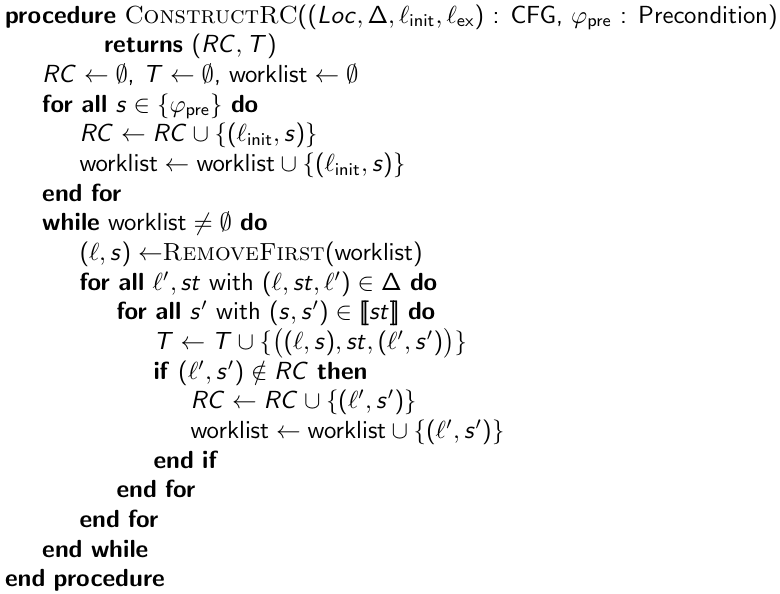
\includegraphics[width=0.7\linewidth]{./figures/explicit_state.png}
			}}
    \item Advantages and disadvantages.
		\framebox[0.90\textwidth][l]{\parbox{0.85\textwidth}{
        \begin{betterlist}
          \item[\color{green}{$\oplus$}] wenn program korrekt ist, dann können wir es auch zeigen (completeness)
          \item[\color{green}{$\oplus$}] can directly read execution from reachability graph
          \item[\color{green}{$\oplus$}] fully automatic
          \item[\color{green}{$\oplus$}] no smt-solver calls
          \item[\color{red}{$\ominus$}] not working for infinite variable domains, no soundness
          \item[\color{red}{$\ominus$}] for large domains might get large
        \end{betterlist}
			}}
		\item Which kinds of specifications can be checked with the technique? E.g. precondition-postcondition pairs, assert statements, no division by zero, termination, ...

		\framebox[0.90\textwidth][l]{\parbox{0.85\textwidth}{
				\begin{betterlist}
					\allpre
				\end{betterlist}
			}}
		\item \alert{Soundness}
		\begin{betterlist}
			\item \underline{For correct programs}
			\begin{betterlist}
				\item In which circumstances does the technique claim that a program is correct?

				\framebox[0.90\textwidth][l]{\parbox{0.85\textwidth}{
						\begin{betterlist}
							\item once it terminates and didn't find an error configuration,
							\begin{betterlist}
								\item one has explicit value, can just insert into postcondition and see if true or false
							\end{betterlist}

						\end{betterlist}
					}}
				\item Existence of false negatives: If the technique claims a program is correct, is the program guaranteed to be correct?

				\framebox[0.90\textwidth][l]{\parbox{0.85\textwidth}{
						\begin{betterlist}
							\item tried out all possibilities, proof by case distinction over all reachable configurations
						\end{betterlist}
					}}
			\end{betterlist}
			\item \underline{For incorrect programs}
			\begin{betterlist}
				\item In which circumstances does the technique claim that a program is incorrect?

				\framebox[0.90\textwidth][l]{\parbox{0.85\textwidth}{
						\begin{betterlist}
							\item if the algorithm finds an error configuration
						\end{betterlist}
					}}
				\item Existence of false positives: If the technique claims a program is incorrect, is the program guaranteed to be incorrect?

				\framebox[0.90\textwidth][l]{\parbox{0.85\textwidth}{
						\begin{betterlist}
							\item no, then one has an execution to a reachable error configuration, in the end a configuration with a state is reachable that shouldn't be reachable
						\end{betterlist}
					}}
			\end{betterlist}
			\item Which assumptions (on the program, or the specification, or the program’s environment) are needed for soundness?
			\framebox[0.90\textwidth][l]{\parbox{0.85\textwidth}{
					\begin{betterlist}
						\item domains for variables finite
					\end{betterlist}

				}}
		\end{betterlist}
		\item \alert{Completeness}
		\begin{betterlist}
			\item \underline{UNKNOWN verdicts} (failing to either establish correctness of incorrectness)
			\begin{betterlist}
				\item Given a correct program, is it possible that the technique terminates with an UNKNOWN verdict? If so, in which cases can this happen?

				\framebox[0.90\textwidth][l]{\parbox{0.85\textwidth}{
						\begin{betterlist}
							\item no, is (sound and) complete for finite variable domains
						\end{betterlist}
					}}
				\item Given an incorrect program, is it possible that the technique terminates with an UNKNOWN verdict? If so, in which cases can this happen?

				\framebox[0.90\textwidth][l]{\parbox{0.85\textwidth}{
						\begin{betterlist}
							\item no, is (sound and) complete for finite variable domains
						\end{betterlist}
					}}
			\end{betterlist}
			\item \underline{Termination}
			\begin{betterlist}
				\item Does the technique always terminate for correct programs? If not, what might the technique do for an infinite amount of time (which step of the algorithm)? In which cases can this occur?

				\framebox[0.90\textwidth][l]{\parbox{0.85\textwidth}{
						\begin{betterlist}
							\item yes, terminates if domain of variables is finite
							\begin{betterlist}
								\item for infinite domains of variables may not terminate, may iterate over infinitely many initial configurations and may add infinitely many configurations while processing the worklist
							\end{betterlist}
						\end{betterlist}
					}}
				\item Does the technique always terminate for incorrect programs? If not, what might the technique do for an infinite amount of time (which step of the algorithm)? In which cases can this occur?

				\framebox[0.90\textwidth][l]{\parbox{0.85\textwidth}{
						\begin{betterlist}
							\item yes and without extension needs same time as for correct program, because algorithm after finding an error configuration continues and only checks later
						\end{betterlist}
					}}
			\end{betterlist}
			\item Are there any programs which the technique does not support at all?

			\framebox[0.90\textwidth][l]{\parbox{0.85\textwidth}{
					\begin{betterlist}
						\item domains of the variables finite
					\end{betterlist}
				}}
		\end{betterlist}
		\item \alert{User Input:} How much / which user input is needed for the technique?
		\begin{betterlist}
			\item \checkboxChecked the program, converted to

			\framebox[0.90\textwidth][l]{\parbox{0.85\textwidth}{
					\begin{betterlist}
						\item CFG
					\end{betterlist}
				}}
			\item \checkboxHalfChecked the specification. Explain: Is the specification high-level or detailed, easy to specify or complex?

			\framebox[0.90\textwidth][l]{\parbox{0.85\textwidth}{
					\begin{betterlist}
						\specpre
					\end{betterlist}
				}}
			\item \checkboxUnchecked suitable settings; e.g. choosing a mode or abstract domain for the given program and specification. Explain: What has to be chosen, and how easy is it to predict useful settings for a given program?

			\framebox[0.90\textwidth][l]{\parbox{0.85\textwidth}{
					-
				}}
			\item \checkboxUnchecked parts of the proof, e.g. invariants. Explain: What has to be given? Does it sometimes suffice to give parts, and the rest can be inferred?

			\framebox[0.90\textwidth][l]{\parbox{0.85\textwidth}{
					-
				}}
			\item \checkboxUnchecked individual steps of the proof, using some proof system. Explain: Which steps can be applied systematically? Where is creativity needed?

			\framebox[0.90\textwidth][l]{\parbox{0.85\textwidth}{
					-
				}}
			\item \checkboxUnchecked the proof is completely manual
			\framebox[0.90\textwidth][l]{\parbox{0.85\textwidth}{
					-
				}}
		\end{betterlist}
		\item \alert{Provided Output}
		\begin{betterlist}
			\item If the technique determines that a program is incorrect, what additional information can be provided to the user? E.g. a failing execution (including variable values), a feasible error trace, any information about why the program is incorrect?

			\framebox[0.90\textwidth][l]{\parbox{0.85\textwidth}{
					\begin{betterlist}
						\item directly get execution as CE
					\end{betterlist}
				}}
			\item If the technique determines that a program is correct, what additional information can be provided to the user? E.g. is there some kind of \enquote{proof artifact} that can be created? If so, is it easy to understand for humans? Is it usable by machines?

			\framebox[0.90\textwidth][l]{\parbox{0.85\textwidth}{
					\begin{betterlist}
						\item one kind of has a proof, because the reachability graph has no error configurations and the reachability graph includes all possible reachable configurations
					\end{betterlist}
				}}
			\item If the technique returns UNKNOWN, what additional information can be provided to the user? Does the information help the user to understand why the result is UNKNOWN? Does it help the user to provide better input that avoids an UNKNOWN verdict?

			\framebox[0.90\textwidth][l]{\parbox{0.85\textwidth}{
					\begin{betterlist}
						\item not possible
					\end{betterlist}
				}}
			\item If the technique does not terminate or runs for a very long time, what information can be provided to help the user understand why?

			\framebox[0.90\textwidth][l]{\parbox{0.85\textwidth}{
					\begin{betterlist}
						\item not possible
					\end{betterlist}
				}}
		\end{betterlist}
		\item \alert{Efficiency}
		\begin{betterlist}
			\item What are the bottlenecks for the technique? Which steps of the algorithm may be particularly inefficient, and in which cases?

			\framebox[0.90\textwidth][l]{\parbox{0.85\textwidth}{
					\begin{betterlist}
						\item if domains of variables large, then needs a lot of memory and time to compute the reachability graph
					\end{betterlist}
				}}
			\item Are there particularly important optimizations?

			\framebox[0.90\textwidth][l]{\parbox{0.85\textwidth}{
					\begin{betterlist}
						\item like for Bounded Model Checking terminate once finding an error configuration
					\end{betterlist}
				}}
		\end{betterlist}
		\item \alert{Further Aspects}
		\begin{betterlist}
			\item \underline{Modularity:} Can the verification for complex programs (or complex specifications) be broken down into verification tasks for smaller parts of the program / parts of the specification? If so, does this allow for efficiency benefits, e.g. parallelization of the sub-verification tasks? Can the modularity help as part of a software development process? E.g. by allowing to verify parts of the program, when other parts have not been written yet?

			\framebox[0.90\textwidth][l]{\parbox{0.85\textwidth}{
					\begin{betterlist}
						\item as long as parts don't influence each other
						\prepostreusetwo
					\end{betterlist}
				}}
			\item \underline{Incrementality:} Can verification artefacts be reused for modified versions of the program? E.g. if the program is still under development.

			\framebox[0.90\textwidth][l]{\parbox{0.85\textwidth}{
					\begin{betterlist}
						\prepostreuse
					\end{betterlist}
				}}
			\item Which techniques are used? E.g. SMT solving, automata, ...

			\framebox[0.90\textwidth][l]{\parbox{0.85\textwidth}{
					\begin{betterlist}
						\item Reachability Graph
						\item relational semantics (via relations for different statements $[[st]]$), just execute statement
					\end{betterlist}
				}}
			\item How much is the overall cost of applying the technique? The cost may depend on how much computing power is needed, but often the cost for human labor (salary for skilled engineers who provide invariants or perform proofs) is much higher
			\framebox[0.90\textwidth][l]{\parbox{0.85\textwidth}{
					\begin{betterlist}
						\item num locations + product of all variable domains in the worst case, but usually lower dependending on precondition and program structure
					\end{betterlist}
				}}
		\end{betterlist}
	\end{betterlist}
\end{minipage}
\begin{minipage}[t]{0.16\linewidth}
	\raggedright
	\fbox{building the precise ARG / Bounded Model Checking}
	\begin{betterlist}
		% \item see page \pageref{pdf:bounded_mode_checking}
		\item Give a short description of the technique
		\framebox[0.90\textwidth][l]{\parbox{0.85\textwidth}{
				\begin{betterlist}
					\item an \alert{abstract (program) configuration} is a pair $(\ell, \{\varphi\})$ where $\ell$ is a location and $\varphi$ is a formula over the program’s variables
					\item an \alert{abstract reachability graph} is a graph $(AC, T)$ where AC is a set of abstract configurations and $T \subseteq AC \times Stmt \times AC$, such that
					\begin{enumerate}
						\item for each edge $((\ell, {\varphi}), st, (\ell', \{\varphi'\})) \in T$, we have $(\ell, st, \ell') \in \Delta$ and $sp(\{\varphi\}, st) \subseteq \{\varphi'\}$,
						\item for each abstract configuration $(\ell, \{\varphi\}) \in AC$ with $\varphi\not\equiv false$ and $(\ell, st, \ell') \in ∆$, there exists an abstract configuration $(\ell', \{\varphi'\}) \in AC$ such that $((\ell, \{\varphi\}), st, (\ell', \{\varphi'\})) \in T$,
						\item there exists $(\ell_{init}, \{\varphi_{init}\}) \in AC$ with $\{\varphi_{pre}\} \subseteq \{\varphi_{init}\}$, and
						\item for each abstract configuration $(\ell, \{\varphi\}) \in AC$ there is a path from $(\ell_{init}, \{\varphi_{init}\})$ to $(\ell, \{\varphi\})$, using edges in $T$
					\end{enumerate}
					\item a \alert{precise abstract reachability graph} is an abstract reachability graph $(AC, T)$ such that for each edge $((\ell, \{\varphi\}), st, (\ell', \{\varphi'\}))$ the equality $sp(\{\varphi\}, st) = \{\varphi'\}$ holds, and $\{\varphi_{init}\} = \{\varphi_{pre}\}$
					\item performs a standard breadth-first traversal of the graph while constructing the graph on the fly
				\end{betterlist}

				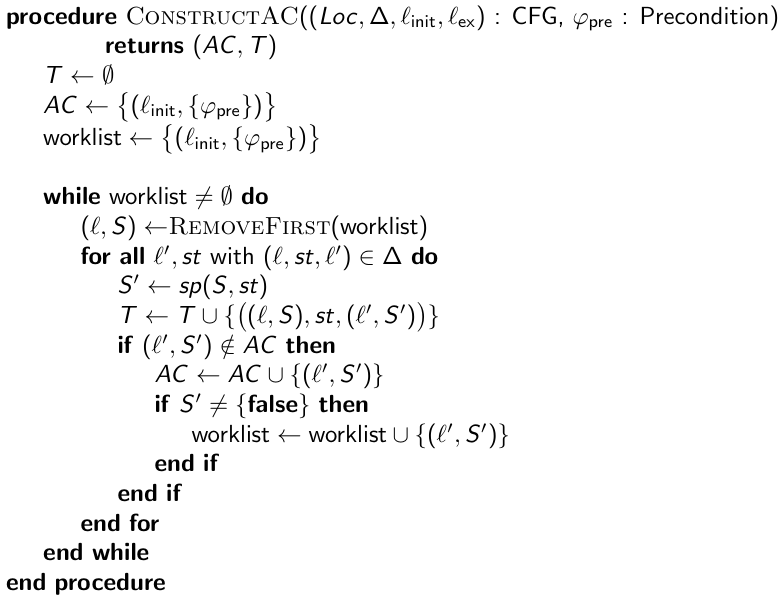
\includegraphics[width=0.7\linewidth]{./figures/bounded_model_checking.png}
			}}
    \item Advantages and disadvantages.
		\framebox[0.90\textwidth][l]{\parbox{0.85\textwidth}{
        \begin{betterlist}
          \item[\color{green}{$\oplus$}] guarentee up to a bound k knows that it's correct
          \item[\color{green}{$\oplus$}] will eventuall find every error
          \item[\color{green}{$\oplus$}] fully automatic
          \item[\color{red}{$\ominus$}] not terminating for programs with loops, not complete
          \item[\color{red}{$\ominus$}] smt-solver to check postconditions for every exit location
        \end{betterlist}
			}}
		\item Which kinds of specifications can be checked with the technique? E.g. precondition-postcondition pairs, assert statements, no division by zero, termination, ...

		\framebox[0.90\textwidth][l]{\parbox{0.85\textwidth}{
				\begin{betterlist}
					\allpre
				\end{betterlist}
			}}
		\item \alert{Soundness}
		\begin{betterlist}
			\item \underline{For correct programs}
			\begin{betterlist}
				\item In which circumstances does the technique claim that a program is correct?

				\framebox[0.90\textwidth][l]{\parbox{0.85\textwidth}{
						\begin{betterlist}
							\item In the case that the algorithm terminates without finding an abstract error configuration, the program is correct
						\end{betterlist}
					}}
				\item Existence of false negatives: If the technique claims a program is correct, is the program guaranteed to be correct?

				\framebox[0.90\textwidth][l]{\parbox{0.85\textwidth}{
						\begin{betterlist}
							\item yes, if algorithm terminates and no abstract error location has been found, then none is reachable
						\end{betterlist}
					}}
			\end{betterlist}
			\item \underline{For incorrect programs}
			\begin{betterlist}
				\item In which circumstances does the technique claim that a program is incorrect?

				\framebox[0.90\textwidth][l]{\parbox{0.85\textwidth}{
						\begin{betterlist}
							\item if the algorithm finds an abstract error configuration
						\end{betterlist}
					}}
				\item Existence of false positives: If the technique claims a program is incorrect, is the program guaranteed to be incorrect?

				\framebox[0.90\textwidth][l]{\parbox{0.85\textwidth}{
						\begin{betterlist}
							\item yes, because $sp(\{\varphi\}, st) = \{\varphi'\}$ and not $\{\varphi_{pre}\} \subseteq \{\varphi_{init}\}$, thus all states reachable over $\{\varphi'\}$ are really reachable and are not just an overapproximation
						\end{betterlist}
					}}
			\end{betterlist}
			\item Which assumptions (on the program, or the specification, or the program’s environment) are needed for soundness?
			\framebox[0.90\textwidth][l]{\parbox{0.85\textwidth}{
					\begin{betterlist}
						\item strongest post correctly defined
					\end{betterlist}
				}}
		\end{betterlist}
		\item \alert{Completeness}
		\begin{betterlist}
			\item \underline{UNKNOWN verdicts} (failing to either establish correctness of incorrectness)
			\begin{betterlist}
				\item Given a correct program, is it possible that the technique terminates with an UNKNOWN verdict? If so, in which cases can this happen?

				\framebox[0.90\textwidth][l]{\parbox{0.85\textwidth}{
						\begin{betterlist}
							\item yes, smt-sovler check for checking subset of postcondition in exit location, can return unknown
							\begin{betterlist}
								\item and if there's a timeout in case that it's going to run infintely or just a too long running example
							\end{betterlist}
						\end{betterlist}
					}}
				\item Given an incorrect program, is it possible that the technique terminates with an UNKNOWN verdict? If so, in which cases can this happen?

				\framebox[0.90\textwidth][l]{\parbox{0.85\textwidth}{
						\begin{betterlist}
							\item no, it will terminate for an incorrect program (that is able to terminate)
						\end{betterlist}
					}}
			\end{betterlist}
			\item \underline{Termination}
			\begin{betterlist}
				\item Does the technique always terminate for correct programs? If not, what might the technique do for an infinite amount of time (which step of the algorithm)? In which cases can this occur?

				\framebox[0.90\textwidth][l]{\parbox{0.85\textwidth}{
						\begin{betterlist}
							\item no, may not terminate, may add infinitely many abstract configurations while processing the worklist
						\end{betterlist}
					}}
				\item Does the technique always terminate for incorrect programs? If not, what might the technique do for an infinite amount of time (which step of the algorithm)? In which cases can this occur?

				\framebox[0.90\textwidth][l]{\parbox{0.85\textwidth}{
						\begin{betterlist}
							\item yes, is always terminating if using breath-first search
						\end{betterlist}
					}}
			\end{betterlist}
			\item Are there any programs which the technique does not support at all?

			\framebox[0.90\textwidth][l]{\parbox{0.85\textwidth}{
					\begin{betterlist}
						\item For most programs with loops, the algorithm does not terminate
					\end{betterlist}
				}}
		\end{betterlist}
		\item \alert{User Input:} How much / which user input is needed for the technique?
		\begin{betterlist}
			\item \checkboxChecked the program, converted to

			\framebox[0.90\textwidth][l]{\parbox{0.85\textwidth}{
					\begin{betterlist}
						\item CFG
					\end{betterlist}
				}}
			\item \checkboxHalfChecked the specification. Explain: Is the specification high-level or detailed, easy to specify or complex?

			\framebox[0.90\textwidth][l]{\parbox{0.85\textwidth}{
					\begin{betterlist}
						\specpre
					\end{betterlist}
				}}
			\item \checkboxUnchecked suitable settings; e.g. choosing a mode or abstract domain for the given program and specification. Explain: What has to be chosen, and how easy is it to predict useful settings for a given program?

			\framebox[0.90\textwidth][l]{\parbox{0.85\textwidth}{
					-
				}}
			\item \checkboxUnchecked parts of the proof, e.g. invariants. Explain: What has to be given? Does it sometimes suffice to give parts, and the rest can be inferred?

			\framebox[0.90\textwidth][l]{\parbox{0.85\textwidth}{
					-
				}}
			\item \checkboxUnchecked individual steps of the proof, using some proof system. Explain: Which steps can be applied systematically? Where is creativity needed?

			\framebox[0.90\textwidth][l]{\parbox{0.85\textwidth}{
					-
				}}
			\item \checkboxUnchecked the proof is completely manual
			\framebox[0.90\textwidth][l]{\parbox{0.85\textwidth}{
					-
				}}
		\end{betterlist}
		\item \alert{Provided Output}
		\begin{betterlist}
			\item If the technique determines that a program is incorrect, what additional information can be provided to the user? E.g. a failing execution (including variable values), a feasible error trace, any information about why the program is incorrect?

			\framebox[0.90\textwidth][l]{\parbox{0.85\textwidth}{
					\begin{betterlist}
						\item Reachability graph directly provides execution to error configuration
					\end{betterlist}
				}}
			\item If the technique determines that a program is correct, what additional information can be provided to the user? E.g. is there some kind of \enquote{proof artifact} that can be created? If so, is it easy to understand for humans? Is it usable by machines?

			\framebox[0.90\textwidth][l]{\parbox{0.85\textwidth}{
					\begin{betterlist}
						\item contains no error configuration, could call a safety proof, because it's also an abstract reachablity graph
					\end{betterlist}
				}}
			\item If the technique returns UNKNOWN, what additional information can be provided to the user? Does the information help the user to understand why the result is UNKNOWN? Does it help the user to provide better input that avoids an UNKNOWN verdict?

			\framebox[0.90\textwidth][l]{\parbox{0.85\textwidth}{
					\begin{betterlist}
						\item precise abstract reachability graph up until this point
						\item \underline{Guarantees correctness up to a bound:}
						\begin{betterlist}
							\item After we explored all nodes whose distance to the initial node is smaller than $k$, we can guarantee the program cannot reach an error by executing less than $k$ statements
						\end{betterlist}
					\end{betterlist}
				}}
			\item If the technique does not terminate or runs for a very long time, what information can be provided to help the user understand why?

			\framebox[0.90\textwidth][l]{\parbox{0.85\textwidth}{
					\begin{betterlist}
						\item same as above
					\end{betterlist}
				}}
		\end{betterlist}
		\item \alert{Efficiency}
		\begin{betterlist}
			\item What are the bottlenecks for the technique? Which steps of the algorithm may be particularly inefficient, and in which cases?

			\framebox[0.90\textwidth][l]{\parbox{0.85\textwidth}{
					\begin{betterlist}
						\item smt-solver check for every exit location that is added is not so relevant
						\item doesn't work for many while loops, doesn't know if it terminates
					\end{betterlist}
				}}
			\item Are there particularly important optimizations?

			\framebox[0.90\textwidth][l]{\parbox{0.85\textwidth}{
					\begin{betterlist}
						\item Check if $(\ell ' , S)$ is an abstract error configuration while adding it to the graph
						\item If $(\ell ' , S)$ is an abstract error configuration, then discontinue to build the graph and tell the user that the program is not safe
						\item Construct a path $(\ell_0, S_0),\ldots , (\ell_0, S_0)$ such that $(\ell_0, S_0)$ is $(\ell_{init}, \{ \varphi_{pre}\} )$ and $(\ell_n, S_n)$ is the abstract error configuration $(\ell' , S)$
						\item Let $st_1,\ldots s_n$ be a sequence of statements such that $(\ell_{i−1}, st_i, \ell_i) \in \Delta$ and $S_i = sp(S_{i−1}, st_i)$ for each $i \in \{1,\ldots, n\}$. Return $st_1,\ldots s_n$ to the user as a counterexample to safety of the program
					\end{betterlist}
				}}
		\end{betterlist}
		\item \alert{Further Aspects}
		\begin{betterlist}
			\item \underline{Modularity:} Can the verification for complex programs (or complex specifications) be broken down into verification tasks for smaller parts of the program / parts of the specification? If so, does this allow for efficiency benefits, e.g. parallelization of the sub-verification tasks? Can the modularity help as part of a software development process? E.g. by allowing to verify parts of the program, when other parts have not been written yet?

			\framebox[0.90\textwidth][l]{\parbox{0.85\textwidth}{
					\begin{betterlist}
						\prepostreusetwo
					\end{betterlist}
				}}
			\item \underline{Incrementality:} Can verification artefacts be reused for modified versions of the program? E.g. if the program is still under development.

			\framebox[0.90\textwidth][l]{\parbox{0.85\textwidth}{
					\begin{betterlist}
						\item yes, can reuse precise abstract reachability graph it if one already executed it up until step $k$ and later parts weren't visited
					\end{betterlist}
				}}
			\item Which techniques are used? E.g. SMT solving, automata, ...

			\framebox[0.90\textwidth][l]{\parbox{0.85\textwidth}{
					\begin{betterlist}
						\item precise Abstract Reachability Graph (precise ARG)
						\item strongest post operator for different statements
						\item breath first search
					\end{betterlist}
				}}
			\item How much is the overall cost of applying the technique? The cost may depend on how much computing power is needed, but often the cost for human labor (salary for skilled engineers who provide invariants or perform proofs) is much higher
			\framebox[0.90\textwidth][l]{\parbox{0.85\textwidth}{
					\begin{betterlist}
						\item for programs that have variables with infinite domains and loops it's unpredictable
					\end{betterlist}
				}}
		\end{betterlist}
	\end{betterlist}
\end{minipage}
\begin{minipage}[t]{0.16\linewidth}
	\raggedright
	\fbox{Abstract Interpretation}
	\begin{betterlist}
		\item Give a short description of the technique
		\framebox[0.90\textwidth][l]{\parbox{0.85\textwidth}{
				\begin{betterlist}
					% \item \underline{Idea of abstraction:}
					% \begin{betterlist}
					% 	\item partition program configurations into finitely many equivalence classes
					% 	\item connect two equivalence classes $C_1$, $C_2$ by an edge if there are configurations $c_1 \in C_1$ and $c_2 \in C_2$ that are connected by an edge
					% 	\item call an equivalence class initial if it contains an initial configuration. Call an equivalence class error if it contains an error configuration
					%        \item can view an abstract state as representing a set of program states that are considered \enquote{equivalent} with respect to the property being analyzed. These concrete states form an equivalence class in the abstract domain
					% 	\item and choose a abstract state for every to  TODO, galois connection, lattice important
					% \end{betterlist}
					\item abstract interpretation simplifies the program's state space by abstracting (or generalizing) detailed information into a more manageable form. This allows it to analyze large programs efficiently, making it scalable even for complex systems
					\begin{betterlist}
						\item \alert{Reduction of State Space:} By grouping these concrete states into equivalence classes, abstract interpretation reduces the number of states that need to be considered. Instead of tracking every possible concrete state individually, the analysis only needs to consider a representative abstract state for each equivalence class. This reduction in the number of states dramatically lowers the computational complexity% efficiency of abstraction to equivalence classes in abstract interpretation comes from reducing the complexity of the program analysis by transforming a large, potentially infinite set of concrete states into a smaller, finite set of abstract states. 
						% \item \alert{Simplification of Operations:} operations on concrete states are replaced by operations on abstract states (equivalence classes). These operations are typically much simpler because they work on generalized representations of the states rather than detailed, exact values
						\item \alert{Avoidance of Path Explosion:} Abstract interpretation merges paths that behave similarly with respect to the properties being analyzed. By grouping paths into equivalence classes, the analysis can reason about all possible executions of a loop or conditional in a single step, rather than separately analyzing each path
						\item \alert{Handling Infinite Domains:} Many programs operate on potentially infinite domains (e.g., all possible integers or all possible memory states). Directly analyzing such domains is infeasible. Abstraction to equivalence classes allows these infinite domains to be represented by a finite set of abstract states, making the analysis tractable
						\item \alert{Focus on Relevant Properties:} Abstraction to equivalence classes allows the analysis to focus on properties that are relevant to the verification goal, ignoring irrelevant details. This selective abstraction reduces the amount of information the analysis needs to track, improving efficiency
					\end{betterlist}
					\item we have so called abstract domains, they define the structure and rules for grouping concrete program states into equivalence classes
					\begin{betterlist}
						\item abstract domain is structured as a complete lattice. The elements of this lattice represent the abstract states. The lattice structure will later be essential for ensuring that the abstract annotation converges to a fixpoint
						\item Galios connection formalizes the relationship between the domain of abstract and concrete states, defining how each element of the concrete domain relates to an element in the abstract domain, it preserves the order relationships between concrete states and abstract states% Galois connections provides the theoretical foundation for the abstraction and concretization processes in abstract interpretation
						\item we are more concrettely using nonrelational abstract domains that do not capture relationships between different program variables. Instead, they focus on analyzing each variable independently
						\item the abstract states of non-relational abstract domains form a complete lattice as defined by the lemma below
						\item an \alert{abstract domain} is a tuple $(\mathbb{A}, \sqsubseteq, \gamma, \alpha)$, such that
						\begin{betterlist}
							\item $(\mathbb{A}, \sqsubseteq)$ is a complete lattice
							\begin{betterlist}
								\item a \alert{complete lattice} is a tuple $(L, \sqsubseteq)$ such that
								\begin{betterlist}
									\item $L$ is a set,
									\item $\sqsubseteq $ is a \alert{partial order} over $L$,
									\item every subset $M$ of $L$ has a \alert{greatest lower bound} $\sqcap M$ w.r.t. $\sqsubseteq$
									\item every subset $M$ of $L$ has a \alert{least upper bound} $\sqcup M$ w.r.t. $\sqsubseteq$
								\end{betterlist}
							\end{betterlist}
							\item $(\alpha, \gamma)$ is a Galois connection for $(\mathbb{A}, \sqsubseteq)$ and $(2^{S_{V ,\mu}}, \subseteq)$
						\end{betterlist}
						\item A value abstraction $(A_{\mathbb{Z}}, \sqsubseteq_{\mathbb{Z}}, \gamma_{\mathbb{Z}}, \alpha_{\mathbb{Z}})$ for $\mathbb{Z}$ induces the \alert{non-relational abstract domain} $(\mathbb{A}, \sqsubseteq, \gamma, \alpha)$ with
						\begin{betterlist}
							\item $\mathbb{A} = V \rightarrow A_{\mathbb{Z}}$
							\item $s^\#_1 \sqsubseteq s^\#_2$ iff for all $x \in V$ it holds that $s^\#_1(x) \sqsubseteq_{\mathbb{Z}} s^\#_2(x)$
							\item $\gamma(s^\#) = \{s \in S_{V ,\mu} | \text{ for all } x \in V, s(x) \in \gamma_{\mathbb{Z}}(s^\#(x))\}$
							\item $\alpha(S) = \{x \mapsto \alpha_{\mathbb{Z}}(\{s(x) | s \in S\}) \mid x \in V\}$
						\end{betterlist}
						\item If $(Y, \sqsubseteq_Y)$ is a complete lattice, and $X$ is any set, then $(X\rightarrow Y, \sqsubseteq)$ is also a complete lattice, where $X \rightarrow Y$ is the set of all functions from $X \rightarrow Y$, and $f \sqsubseteq g$ iff for all $x \in X$, we have $f(x) \sqsubseteq_Y g(x)$
					\end{betterlist}
					\item have abstract annotation which intuitively gives us the abstract states we should add to each location of the control flow graph in order to get an ARG (and thus maybe a safety proof if no error configurations are reachable, the ARGs will have the same structure as the underlying CFG)%. The set of program states is represented as an abstract state
					\begin{betterlist}
						\item abstract annotations were defined via a recursive equation system (in an ARG every set of states has to be subset of the strongest post of the previous set of states, that is the equation system)
						\item For every abstract domain, the function $Loc \rightarrow \mathbb{A}_S$ (possible abstract annotation) forms a complete lattice by the lemma above
						\item for a CFG $(Loc, \Delta, \ell_{init}, \ell_{ex})$, an abstract annotation is a function $f: Loc \rightarrow \mathbb{A}_S$ which satisfies $f(\ell_{init}) \sqsupseteq \alpha(\{\varphi_{pre}\}) \sqcup \bigsqcup \{post^\#(f(\ell'), st) \mid (\ell′, st, \ell_{init}) \in \Delta\}$ and for all $\ell \in Loc \setminus \{\ell_{init}\}$, $f(\ell) \sqsupseteq \bigsqcup \{post^\#(f(\ell'), st) \mid (\ell', st, \ell) \in \Delta\}$
					\end{betterlist}
					% \item any abstract annotation defines an abstract reachability graph. 
					\item by using theory if fixpoints and lattices one can guarantee there always exist a solution to such an equation system that can be computed in finite time
					\begin{betterlist}
						\item every complete lattice and thus also the function $Loc \rightarrow \mathbb{A}_S$ (possible abstract annotation) has a fixpoint when inserted into an arbitrary monotone function as it is proven by the Knaster Tarksi fixpoint theorem, the complete lattice's structure allows us to construct the least fixed point by taking the least upper bound of elements that are "below" their image under the function (and similarly construct the greatest fixed point by taking the greatest lower bound of elements that are "above" their image), the greatst upper bound of these elements exists because a complete lattice has a least upper bound for every subset of it's domain
						\item the function $Loc \rightarrow \mathbb{A}_S$ (possible abstract annotation) represents the abstract states that a program can reach in it's execution, unfortunetely the Kanster Tarski fixpoint theorem does not guarantee that we can compute the fixpoint in finite time, in case of e.g. the interval domain it could be unreachable like $[-\infty, \infty]$
						\item therefore we have the Theorem ACC-FP, it guarantess that we can reach a fixpiont of the monotone function $F^\#  : (Loc \rightarrow \mathbb{A}_S) \rightarrow (Loc \rightarrow \mathbb{A}_S)$ / we can compute a abstract annotation in finite time, by repeated application of $F^\#$, in case that the lattice (nonrelational abstract states $\mathbb{A}_S$) on which the function $F^\#$ operates satisfies the ACC
						\begin{betterlist}
							\item thus in order to guarantee termination in all cases (all possible starting points of the function $Loc \rightarrow \mathbb{A}_S$ (possible abstract annotation)), we require that the lattice satisfies the ACC
							\item by the lemma below the abstract states of non-relational abstract domains $\mathbb{A}_S$ and thus also the function $Loc \rightarrow \mathbb{A}_S$ (possible abstract annotation) satisfy the ACC, because explicit value domain (latest after 3 steps) and sign domain (latest after 5 steps) do
							\item the function $F^\#$ is monotone, because $\sqsubseteq$ is the case for all abstract states of the locations and the function $F^\#$ only applies least upper bound to all operators
						\end{betterlist}
						\item in order to be sure to overapproximate as little as possible with our abstract annotation, as our function $F^\#$ is continous, we can use the Kleene Fixpoint Theorem, to guarantee that the fixpoint we reach is the least fixpoint of the function $F^\#$%, thus the fixpoint we reach is the most precise abstract annotation
						\item an abstract annotation is a fixpoint of the monotone function $F_\#  : (Loc \rightarrow \mathbb{A}_S) \rightarrow (Loc \rightarrow \mathbb{A}_S)$ with:\\$F^\# (g) = \left\{\ell_{init} \mapsto g(\ell_{init}) \sqcup \alpha(\{\varphi_{pre}\}) \sqcup \bigsqcup \{post^\#(g(\ell'), st) \mid (\ell', st, \ell_{init}) \in \Delta \}\right\}$\\$\cup  \left\{\ell \mapsto g(\ell) \sqcup  \bigsqcup \{post^\#(g(\ell'), st) \mid (\ell', st, \ell) \in \Delta \} | \ell \in Loc \setminus \{ \ell init\}\right\}$
							\item \alert{Knaster-Tarski Fixpoint Theorem}: Let $(X, \sqsubseteq)$ be a complete lattice. If $f:X \rightarrow X$ is monotone then $f$ has a least fixpoint and this fixpoint is $\bigsqcap \{x \mid f(x) \sqsubseteq x\}$
							\item \underline{Kleene Chains:} Let $F : X \rightarrow X$ be a monotone function in a complete lattice $(X, \sqsubseteq)$, and let $\bot = \bigsqcap X$ be the least element of $X$
						\begin{betterlist}
							\item it holds that $\bot\sqsubseteq F(\bot) \sqsubseteq \ldots \sqsubseteq F^n(\bot) \sqsubseteq F^{n+1}(\bot) \sqsubseteq \ldots$
							\item \alert{Ascending Chain Condition (ACC)}: $(X, \sqsubseteq)$ satisfies the \alert{ascending chain condition} if for every infinite ascending chain $x_1 \sqsubseteq x_2 \sqsubseteq \ldots$ there exists an $k \in \mathbb{N}$ such that $x_m = x_k$ for all $m \ge k$
							\begin{betterlist}
								\item If a complete lattice $(Y , \sqsubseteq_Y)$ satisfies the ACC, then for any finite set $X$, the complete lattice $(X \rightarrow Y , \sqsubseteq)$ also satisfies the ACC
							\end{betterlist}
							\item \alert{ACC-FP}: If $(X, \sqsubseteq)$ satisfies the ACC, then $\bigsqcup\{F^n(\bot) \mid n \in  \mathbb{N}\}$ is a fixpoint of $F$ and can be computed in finite time
							\item \alert{Kleene Fixpoint Theorem}: If $F$ is continuous (i.e. $F(\bigsqcup M) = \bigsqcup \{F(m) \mid m \in M\}$ for every set $M$), then $\bigsqcup\{F^n(\bot) \mid n \in \mathbb{N}\}$ is the least fixpoint of $F$
						\end{betterlist}
					\end{betterlist}
					\item to ensure termination in abstract domains that do not satisfy the ACC, we introduce widening (interval domain does not satisfy ACC, because it has many infinite ascending chains that don't reach a repeating value: $[0, 1] \sqsubseteq [0, 2]\sqsubseteq [0, 3]\sqsubseteq [0, 4]\ldots$)
					\begin{betterlist}
						\item the widening operator $\triangledown$ is an over approximation of the union and of the upper bound so one gets something bigger possibly and one is guaranteed by the second condition that one cannot infinitely often get something bigger at some point it will stay the same and using that one can then show that the kleene iteration with this function always terminates just relatively straightforward from the second condition of the widening operator and the result that one computes is still this kind of abstract annotation that one needed to build an abstract reachability graph and to show that it's still an abstract annotation one use the first condition of the winding operator because one overapproximates the least upper bound it's still fine
						\item a \alert{widening operator} for an abstract domain $(\mathbb{A}_S, \sqsubseteq, \alpha, \gamma)$ is a binary operator $\triangledown$ on abstract states such that:
						\begin{betterlist}
							\item for all $s^\#_1, s^\#_2 \in \mathbb{A}_S$, we have $\gamma(s^\#_1) \cup \gamma(s^\#_2) \subseteq \gamma(s^\#_1 \triangledown s^\#_2)$, and
							\item for any sequence $(s^\#_i)_{i\in \mathbb{N}}$ of abstract states, the sequence $(\tilde s^\#_i)_{i\in \mathbb{N}}$ with $\tilde s^\#_0 = s^\#_0$ and $\tilde s^\#_{i+1} = \tilde s^\#_i \triangledown s^\#_i$ stabilizes; i.e., there exists $n$ such that $\tilde s^\#_m = \tilde s^\#_n$ for all $m \ge n$
						\end{betterlist}
						\item Kleene iteration with $F_{\triangledown}$ always terminates. The result is an abstract annotation: $F_{\triangledown}: (Loc \rightarrow \mathbb{A}_S) \rightarrow (Loc \rightarrow \mathbb{A}_S)$ with $F_{\triangledown}(g) = \{\ell_{init} \mapsto g(\ell_{init}) \triangledown(\alpha(\{\varphi_{pre}\}) \sqcup \bigsqcup \{post^\#(g(\ell'), st) \mid (\ell', st, \ell_{init}) \in \Delta\})\}\cup \{\ell\mapsto g(\ell) \triangledown \bigsqcup\{post^\#(g(\ell'), st) \mid (\ell', st, \ell) \in \Delta\} \mid \ell \in Loc \setminus \{\ell_{init}\}\}$
					\end{betterlist}
					% \item one abstractly interprets programs using an abstract domain and an abstract post operator
					% \item one defines abstract annotations using an equation system and if one has an equation system one can build an abstract reability graph and one can find a solution to this equation system using for instance kleene iteration using one of these two functions $F_\#$ (monotone function over locations mapped to abstract states with least upper bound) or $F_{\triangledown}$ (monotone function over locations mapped to abstract states with widening operator $\triangledown$)
					% \begin{betterlist}
					%   \item the widening operator $\triangledown$ is an over approximation of the union and of the upper bound so one gets something bigger possibly and one is guaranteed by the second condition that one cannot infinitely often get something bigger at some point it will stay the same and using that one can then show that the kleene iteration with this function always terminates just relatively straightforward from the second condition of the widening operator and the result that one computes is still this kind of abstract annotation that one needed to build an abstract reachability graph and to show that it's still an abstract annotation one use the first condition of the winding operator because one overapproximates the least upper bound it's still fine
					% \end{betterlist}
				\end{betterlist}
			}}
    \item Advantages and disadvantages.
		\framebox[0.90\textwidth][l]{\parbox{0.85\textwidth}{
        \begin{betterlist}
          \item[\color{green}{$\oplus$}] always terminates for correct domain that is complete lattice and satisfies ACC and for some rare cases for normal complete lattices
          \item[\color{red}{$\ominus$}] domain muss passend gewählt werden, not complete (not fully automatic)
          \item[\color{red}{$\ominus$}] overapproximation, can only say correct or unknown
          \item[\color{red}{$\ominus$}] smt-solver calls for strongest post
          \item[\color{red}{$\ominus$}] abstract strongest post might by costly, smt-solver call
          \item[\color{red}{$\ominus$}] for incorrect program one can get a possible error trace, but one doesn't know if it's really a error trace, because of overapproximation
        \end{betterlist}
			}}
		\item Which kinds of specifications can be checked with the technique? E.g. precondition-postcondition pairs, assert statements, no division by zero, termination, ...

		\framebox[0.90\textwidth][l]{\parbox{0.85\textwidth}{
				\begin{betterlist}
					% \item assumes precondition and postcondition pair, but Program with assert statements can be converted to only need precondition and postcondition pair
					% \begin{betterlist}
					% 	\item No division by zero thus also possible
					% \end{betterlist}
					\allpre
				\end{betterlist}
			}}
		\item \alert{Soundness}
		\begin{betterlist}
			\item \underline{For correct programs}
			\begin{betterlist}
				\item In which circumstances does the technique claim that a program is correct?

				\framebox[0.90\textwidth][l]{\parbox{0.85\textwidth}{
						\begin{betterlist}
							\item if the ARG is a safety proof, then one has proven the program correct
						\end{betterlist}
					}}
				\item Existence of false negatives: If the technique claims a program is correct, is the program guaranteed to be correct?

				\framebox[0.90\textwidth][l]{\parbox{0.85\textwidth}{
						\begin{betterlist}
							\item yes in the case $phi_{exit} \cap \phi_{post} = \phi_{exit}$, because then there's no error trace, there's no way to reach an abstract error configuration in the ARG
							\begin{betterlist}
								\item if there is no path from an initial equivalence class to an error equivalence class, there is also no path from an initial configuration to an error configuration and the analyzed program is correct
							\end{betterlist}
						\end{betterlist}
					}}
			\end{betterlist}
			\item \underline{For incorrect programs}
			\begin{betterlist}
				\item In which circumstances does the technique claim that a program is incorrect?

				\framebox[0.90\textwidth][l]{\parbox{0.85\textwidth}{
						\begin{betterlist}
							\item never, cannot use it to find errors, so if the program is incorrect one will always end up with some abstract reachability graph that's not a safety proof but one is never sure that something is really an error
							\begin{betterlist}
								\item true positive only in case $\phi_{exit} \cap \phi_{post} = \emptyset$, but mostly it is $\phi_{exit} \cap \phi_{post} = \phi_{exit \cap post}$, thus if there is a path from an initial equivalence class to an error equivalence class, the program might be incorrect but it might also be the case the we have chosen a partition that is not helpful, thus in general one says there are no true positives or false positives
							\end{betterlist}
							\item this can happen, because the abstract post operator overapproximates and one doesn't know if the nonempty difference from $\phi_{post}$ is a result of this overapproximation
							\begin{betterlist}
								\item An \alert{abstract post operator} $post^\#$ for an abstract domain $(\mathbb{A}, \sqsubseteq, \gamma, \alpha)$ is a monotone function that takes an abstract state $s^\# \in \mathbb{A}$ and a simple statement $st$ and returns a new abstract state, such that the following holds: $sp(\gamma(s^\#), st) = post(\gamma(s^\#), [[st]]) \subseteq \gamma(post^\#(s^\#, st))$
							\end{betterlist}
						\end{betterlist}
					}}
				\item Existence of false positives: If the technique claims a program is incorrect, is the program guaranteed to be incorrect?

				\framebox[0.90\textwidth][l]{\parbox{0.85\textwidth}{
						\begin{betterlist}
							\item no false positives, because it is never claimed that the program is incorrect (no true positives)
						\end{betterlist}
					}}
			\end{betterlist}
			\item Which assumptions (on the program, or the specification, or the program’s environment) are needed for soundness?
			\framebox[0.90\textwidth][l]{\parbox{0.85\textwidth}{
					\begin{betterlist}
						\item depends on whether the domain is really suitable for the program and the property one is trying to prove and if it's not then there are limited number of interesting things that one can probably show with the sign domain or the intervals but for other things one needs more expressive domains
						\item non-relational domain has to satisfy Ascending Chain Condition (ACC)
						\begin{betterlist}
							\item sign abstraction satisfies ACC
							\item explicit-value abstraction satisfies ACC
							\item but interval abstraction does not satisfy ACC
							\begin{betterlist}
								\item  if two bounds are not equal one is extreme and says plus infinity to minus infinity after that one can definitely not get bigger anymore, that's one thing one can. Maybe one doesn't want to do this directly one can have some conditions so maybe only if the bounds are greater than 100 or less than minus 100 for this lower bound then one does this extreme widening
								\item or sometimes one has an abstract domain that in addition to the interval it counts how often the interval has gotten bigger and only after it has gotten bigger 10 times then one goes to the extreme plus minus infinity so one wants to limit this somehow, not always be so extreme but in in principle this is how one can do widening for intervals
							\end{betterlist}

						\end{betterlist}
					\end{betterlist}
				}}
		\end{betterlist}
		\item \alert{Completeness}
		\begin{betterlist}
			\item \underline{UNKNOWN verdicts} (failing to either establish correctness of incorrectness)
			\begin{betterlist}
				\item Given a correct program, is it possible that the technique terminates with an UNKNOWN verdict? If so, in which cases can this happen?

				\framebox[0.90\textwidth][l]{\parbox{0.85\textwidth}{
						\begin{betterlist}
							\item the inclusion check for postcondition could fail, smt-solver could return unknown
							\item yes, sometimes if one wants to proof correctness one does not get an ARG that is a safety proof, because the non-relational abstract domain is too weak, as explained above under incorrect programs
						\end{betterlist}
					}}
				\item Given an incorrect program, is it possible that the technique terminates with an UNKNOWN verdict? If so, in which cases can this happen?

				\framebox[0.90\textwidth][l]{\parbox{0.85\textwidth}{
						\begin{betterlist}
							\item the inclusion check for postcondition could fail, smt-solver could return unknown
							\item for incorrect programs it always terminates with UNKNOWN, one gets an ARG that's not a safety proof but one is never sure that something is really an error, the concrete cases were explained above under incorrect programs
						\end{betterlist}
					}}
			\end{betterlist}
			\item \underline{Termination}
			\begin{betterlist}
				\item Does the technique always terminate for correct programs? If not, what might the technique do for an infinite amount of time (which step of the algorithm)? In which cases can this occur?

				\framebox[0.90\textwidth][l]{\parbox{0.85\textwidth}{
						\begin{betterlist}
							\item guaranteed to terminate after finitely many steps, usually one instantiated it such that it terminates, possibly with widening
							\item may also terminate if non-relational abstract domain doesn't satisfy ACC, if one is lucky and there's an upper bound like in this one example from the lecture
						\end{betterlist}
					}}
				\item Does the technique always terminate for incorrect programs? If not, what might the technique do for an infinite amount of time (which step of the algorithm)? In which cases can this occur?

				\framebox[0.90\textwidth][l]{\parbox{0.85\textwidth}{
						\begin{betterlist}
							\item yes, but it will never say that it's an incorrect program
						\end{betterlist}
					}}
			\end{betterlist}
			\item Are there any programs which the technique does not support at all?

			\framebox[0.90\textwidth][l]{\parbox{0.85\textwidth}{
					\begin{betterlist}
						\item it always terminates, but it may or not be may not be a safety proof as the choice of the abstract domain really matters a lot
						\item see CEGAR and Trace Abstraction Refinement
					\end{betterlist}
				}}
		\end{betterlist}
		\item \alert{User Input:} How much / which user input is needed for the technique?
		\begin{betterlist}
			\item \checkboxChecked the program, converted to

			\framebox[0.90\textwidth][l]{\parbox{0.85\textwidth}{
					\begin{betterlist}
						\item CFG
					\end{betterlist}
				}}
			\item \checkboxHalfChecked the specification. Explain: Is the specification high-level or detailed, easy to specify or complex?

			\framebox[0.90\textwidth][l]{\parbox{0.85\textwidth}{
					\begin{betterlist}
						\specpre
						% \item assert statements or prec-post-condition pair is correct, one has to think what is actually the specification that the program should satisfy, formalsing requirements can be a difficult task
					\end{betterlist}
				}}
			\item \checkboxChecked suitable settings; e.g. choosing a mode or abstract domain for the given program and specification. Explain: What has to be chosen, and how easy is it to predict useful settings for a given program?

			\framebox[0.90\textwidth][l]{\parbox{0.85\textwidth}{
					\begin{betterlist}
						\item the choice of the abstract domain really matters a lot
					\end{betterlist}
				}}
			\item \checkboxUnchecked parts of the proof, e.g. invariants. Explain: What has to be given? Does it sometimes suffice to give parts, and the rest can be inferred?

			\framebox[0.90\textwidth][l]{\parbox{0.85\textwidth}{
					-
				}}
			\item \checkboxUnchecked individual steps of the proof, using some proof system. Explain: Which steps can be applied systematically? Where is creativity needed?

			\framebox[0.90\textwidth][l]{\parbox{0.85\textwidth}{
					-
				}}
			\item \checkboxUnchecked the proof is completely manual
			\framebox[0.90\textwidth][l]{\parbox{0.85\textwidth}{
					-
				}}
		\end{betterlist}
		\item \alert{Provided Output}
		\begin{betterlist}
			\item If the technique determines that a program is incorrect, what additional information can be provided to the user? E.g. a failing execution (including variable values), a feasible error trace, any information about why the program is incorrect?

			\framebox[0.90\textwidth][l]{\parbox{0.85\textwidth}{
					\begin{betterlist}
						\item does never determine that Program is incorrect, but one gets a ARG that is not a safety proof
					\end{betterlist}
				}}
			\item If the technique determines that a program is correct, what additional information can be provided to the user? E.g. is there some kind of \enquote{proof artifact} that can be created? If so, is it easy to understand for humans? Is it usable by machines?

			\framebox[0.90\textwidth][l]{\parbox{0.85\textwidth}{
					\begin{betterlist}
						\item always get an abstract reachability graph without error configurations and thus without error traces and thus one gets a safety proof
					\end{betterlist}
				}}
			\item If the technique returns UNKNOWN, what additional information can be provided to the user? Does the information help the user to understand why the result is UNKNOWN? Does it help the user to provide better input that avoids an UNKNOWN verdict?

			\framebox[0.90\textwidth][l]{\parbox{0.85\textwidth}{
					\begin{betterlist}
						\item one gets a reachability graph that is no safety proof, one can try to find a better abstract domain
					\end{betterlist}
				}}
			\item If the technique does not terminate or runs for a very long time, what information can be provided to help the user understand why?

			\framebox[0.90\textwidth][l]{\parbox{0.85\textwidth}{
					\begin{betterlist}
						\item always terminates, see section about termination of correct programs
					\end{betterlist}
				}}
		\end{betterlist}
		\item \alert{Efficiency}
		\begin{betterlist}
			\item What are the bottlenecks for the technique? Which steps of the algorithm may be particularly inefficient, and in which cases?

			\framebox[0.90\textwidth][l]{\parbox{0.85\textwidth}{
					\begin{betterlist}
						\item abstract strongest post might by costly, smt-solver call
						\item call to smt-solver for checking strongest post for every error location
					\end{betterlist}

					% \begin{betterlist}
					% \item the computation of $post^\#$ might be costly like in CEGAR
					% \end{betterlist}
				}}
			\item Are there particularly important optimizations?

			\framebox[0.90\textwidth][l]{\parbox{0.85\textwidth}{
					\begin{betterlist}
						\item \alert{Widening:} start widening after a few iterations (problem of exercise) even if abstract domains satisfies ACC already
						\begin{betterlist}
							\item widening also allows faster termination but may also lead to less precision
						\end{betterlist}
						\item \alert{Predicate Abstraction} (relational domains and not only non-relatonal) is a way to design custom domain, one just picks a set of predicates, a set of formulas and those are the abstract states that one uses, one gets this suitable formulas with the help of infeasability proofs
						\begin{betterlist}
							\item  instead of figuring out this complicated problem of which formulas does one need to prove that the entire program is correct one first figures out a much simpler problem which formulas one needs to prove that one particular sequence of statements, so one particular trace is correct
							\item since one is looking at traces that lead to error locations, correctness really means that they're invasible, they cannot be executed. One can compute invisibility proofs with the weakest precondition or the strongest post condition and one can just do that directly or one could abstract some of the statements to get simpler proofs in the hope that this would be somewhat nicer for the purpose
							\item one has to figure out which of the statements one can abstract and still get an infeasible trace, if one abstracts too much everything becomes feasiable, to check feasability one uses SSA of a trace (one encodes a sequence of statements as a set of formulas), there's a bit of non-determinism in here, it depends on which unsatisfiable core the smt solver is going to give one, deciding which of these proofs one will get
							\item see CEGAR
						\end{betterlist}
					\end{betterlist}
				}}
		\end{betterlist}
		\item \alert{Further Aspects}
		\begin{betterlist}
			\item \underline{Modularity:} Can the verification for complex programs (or complex specifications) be broken down into verification tasks for smaller parts of the program / parts of the specification? If so, does this allow for efficiency benefits, e.g. parallelization of the sub-verification tasks? Can the modularity help as part of a software development process? E.g. by allowing to verify parts of the program, when other parts have not been written yet?

			\framebox[0.90\textwidth][l]{\parbox{0.85\textwidth}{
					\begin{betterlist}
						\item yes, if one variable doesn't get influcended by other part of program and wouldn't have to be updated
					\end{betterlist}
				}}
			\item \underline{Incrementality:} Can verification artefacts be reused for modified versions of the program? E.g. if the program is still under development.

			\framebox[0.90\textwidth][l]{\parbox{0.85\textwidth}{
					\begin{betterlist}
						\item yes, if one variable doesn't get influcended by changes to program and wouldn't have to be updated
					\end{betterlist}
				}}
			\item Which techniques are used? E.g. SMT solving, automata, ...

			\framebox[0.90\textwidth][l]{\parbox{0.85\textwidth}{
					\begin{betterlist}
						\item basically just application of abstract strongest post
						\item Abstract Reachability Graph (ARG)
					\end{betterlist}
				}}
			\item How much is the overall cost of applying the technique? The cost may depend on how much computing power is needed, but often the cost for human labor (salary for skilled engineers who provide invariants or perform proofs) is much higher.

			\framebox[0.90\textwidth][l]{\parbox{0.85\textwidth}{
					\begin{betterlist}
						\item can be made quite efficient
					\end{betterlist}
				}}
		\end{betterlist}
	\end{betterlist}
\end{minipage}

\newpage

\begin{minipage}[t]{0.16\linewidth}
	\raggedright
	\fbox{CEGAR with Predicate Abstraction}
	\begin{betterlist}
		\item Give a short description of the technique.

		\framebox[0.90\textwidth][l]{\parbox{0.85\textwidth}{
				\begin{betterlist}
					\item best explained over it's acronym: counterexample guided abstraction refinement
					\item built an abstraction of the program, an abstract reability graph but one donesn't just build one, we refine it, ons starts with a very abstract reability graph where one just says everywhere all states are possible and then one found some new formulas that allow to rule out some states and one built a more refined and more precise abstract reachability graph and one does this in every iteration, so this is why it's an abstraction refinement
					\item and it's counter example guided because these error traces are counter examples in the sense that they show why the current abstract reability graph is not a safety proof and one use them to guide ones refinement because one basically does the refinement by constructing these infeasability proofs for counter examples
					\item \underline{Steps:}
					\begin{enumerate}
						\item Set $B$ to the empty set
						\item Construct an abstract reachability graph ARG that is precise for $B$
						\item Check if ARG is a safety proof
						\begin{betterlist}
							\item If yes, report that P satisfies its specification and return
							\item If no, construct an error trace $\pi$ of ARG
						\end{betterlist}
						\item Check if $\pi$ is feasible
						\begin{betterlist}
							\item If yes, report that $P$ does not satisfy its specification, construct an execution for $\pi$, and return
							\item If no, construct a proof of infeasibility $\varphi_0,\ldots, \varphi_n$ for $\pi$, add the set of formulas $\{\varphi_0,\ldots, \varphi_n\}$ to $B$, and continue with Step 2
						\end{betterlist}
					\end{enumerate}

					\includegraphics[width=\linewidth]{./figures/cegar_approach.png}
					\item \underline{Predicate Abstraction:} Approach to design a customized abstract domain. The abstract domain will be based on a set of formulas $B$. If the set of formulas B was \enquote{good}, the abstract reachability graph will be a safety proof
					\begin{betterlist}
						\item the Hoare proof system allows us to give a correctness proof if we guess \enquote{good} loop invariants. ARGs allow us to give a correctness proof if we guess “good” abstract configurations
						\item we call an abstract reachability graph $(AC, T)$ \alert{precise for $B$} if for each edge $((\ell, \{\varphi\}), st, (\ell', \{\varphi'\})) \in T$ the equality $sp^\#_B(\{\varphi\}, st) = \{\varphi'\}$ holds
					\end{betterlist}

					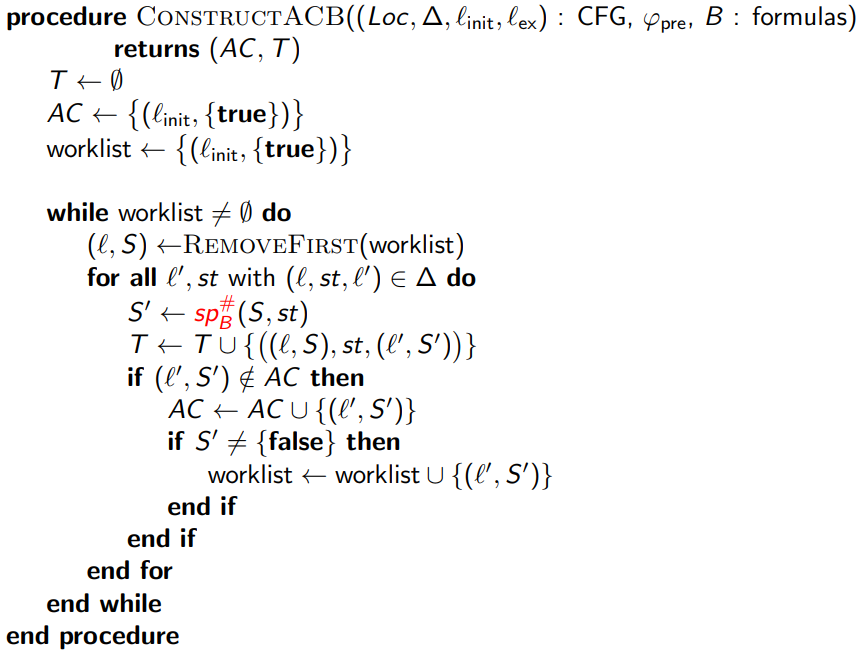
\includegraphics[width=0.7\linewidth]{./figures/ConstructACB.png}
					% \item to find formulas that should be added to $B$, get formulas of the error trace in the ARG precise for $B$, these formulas correpsond to the SSA of the error trace and try to find minimal unsatisfiable core, add formulas of minimal unsatisfiable core to $B$
					\item to find formulas that should be added to $B$, find an error trace in the ARG precise for $B$ and construct the SSA of these formulas (one can't take the formulas from the ARG precise for $B$, because these formulas don't include primes for the order in which statements are executed) and try to find minimal unsatisfiable core, abstract all formulas not in the minimal unsatisfiable core and create a proof of infeasability, add formulas from this proof of infeasability to $B$
					\begin{betterlist}
            \item \alert{Cegar was man da macht, um B zu bekommen:} nicht Formeln von Floyd Hoare annotation nehmen, sondern trace zu error location nehmen und in SSA bringen, erstmal feasiblity check, wenn negativ, dann minimal unsatisfiable core berechnen, alle Statements die nicht im core sind abstrahieren, dann strongest post auf auf abstraction des trace ausführen, angefangen mit true und sich ergebende Formlen dem Set B hinzufügen
						\item We define the \alert{static single-assignment form (SSA)} as the set of formulas $SSA(\pi) := \{\psi_1, \ldots, \psi_n\}$, where

						$\psi_i =
							\begin{cases}
								expr\;\sigma_i                                    & \text{if } st_i \text{ is  assume expr} \\
								\sigma_i(x) = (expr\;\sigma_{i−1})                & \text{if } st_i \text{ is  x:=expr}     \\
								\sigma_i(a) = (a⟨k \triangleleft v⟩) \sigma_{i−1} & \text{if } st_i \text{ is  a[k]:=v}     \\
								true                                              & \text{if } st_i \text{ is  havoc x}
							\end{cases}$
						\begin{betterlist}
							\item $\bigwedge SSA(\pi )$ is unsatisfiable iff $\pi$ is infeasible
						\end{betterlist}
						\item Given a finite set of formulas $\mathbb{F}$ where $\bigwedge \mathbb{F}$ is unsatisfiable, we call a subset $X \subseteq \mathbb{F}$ an \alert{unsatisfiable core} if $\bigwedge X$ is also unsatisfiable
						\begin{betterlist}
							\item An unsatisfiable core $X$ is \alert{minimal} if no strict subset of $X$ is an unsatisfiable core
						\end{betterlist}
					\end{betterlist}
				\end{betterlist}
			}}
    \item Advantages and disadvantages.
		\framebox[0.90\textwidth][l]{\parbox{0.85\textwidth}{
        \begin{betterlist}
          \item[\color{green}{$\oplus$}] terminates for incorrect programs
          \item[\color{green}{$\oplus$}] can return feasible trace and thus a exceution leading to an error location
          \item[\color{green}{$\oplus$}] is fully automatic
          \item[\color{red}{$\ominus$}] not terminating for all programs (not complete)
          \item[\color{red}{$\ominus$}] the bigger B is the more abstract strongest post calls, besides that also for feasability check
          \item[\color{red}{$\ominus$}] the bigger B, the bigger the abstract reachability graph, memory comsumption
          \item[\color{red}{$\ominus$}] running time can vary a lot depending on how fast the right set B is found
          \item[\color{red}{$\ominus$}] hard to decide, which minimal unsatisfiable core is the best one, leading to best formulas
        \end{betterlist}
			}}
		\item Which kinds of specifications can be checked with the technique? E.g. precondition-postcondition pairs, assert statements, no division by zero, termination, ...
		\framebox[0.90\textwidth][l]{\parbox{0.90\textwidth}{
				\begin{betterlist}
					\item same as for Trace Abstraction Refinement
				\end{betterlist}
			}}
		\item \alert{Soundness}
		\begin{betterlist}
			\item \underline{For correct programs}
			\begin{betterlist}
				\item In which circumstances does the technique claim that a program is correct?

				\framebox[0.90\textwidth][l]{\parbox{0.85\textwidth}{
						\begin{betterlist}
							\item same as for Abstract Interpretation
						\end{betterlist}
					}}
				\item Existence of false negatives: If the technique claims a program is correct, is the program guaranteed to be correct?

				\framebox[0.90\textwidth][l]{\parbox{0.85\textwidth}{
						\begin{betterlist}
							\item yes, then it is correct
						\end{betterlist}
					}}
			\end{betterlist}
			\item \underline{For incorrect programs}
			\begin{betterlist}
				\item In which circumstances does the technique claim that a program is incorrect?

				\framebox[0.90\textwidth][l]{\parbox{0.85\textwidth}{
						\begin{betterlist}
							\item if a feasible trace is found
						\end{betterlist}
					}}
				\item Existence of false positives: If the technique claims a program is incorrect, is the program guaranteed to be incorrect?

				\framebox[0.90\textwidth][l]{\parbox{0.85\textwidth}{
						\begin{betterlist}
							\item yes, then it is incorrect
						\end{betterlist}
					}}
			\end{betterlist}
			\item Which assumptions (on the program, or the specification, or the program’s environment) are needed for soundness?
			\framebox[0.90\textwidth][l]{\parbox{0.85\textwidth}{
					\begin{betterlist}
						\item no special requirements
						\item (correctly specified requirements via assert statements or pre-post-condition pairs)
					\end{betterlist}
				}}
		\end{betterlist}
		\item \alert{Completeness}
		\begin{betterlist}
			\item \underline{UNKNOWN verdicts} (failing to either establish correctness of incorrectness)
			\begin{betterlist}
				\item Given a correct program, is it possible that the technique terminates with an UNKNOWN verdict? If so, in which cases can this happen?

				\framebox[0.90\textwidth][l]{\parbox{0.85\textwidth}{
						\begin{betterlist}
							\item yes, if feasibility check returns unknown, whole algorithm returns unknown
							\item if asking whether a given trace $\pi$ is feasible, do a SSA encoding and ask an smt whether this is satisfiable and the smt solver might return unknown
							\begin{betterlist}
								\item depending on what logic one needs to encode the trace if the program uses multiplication and one needs to use a nonlinear arithmetic then this is an undecidable logic, the smt solver will in some cases say that it can't tell whether this trace is feasible or not. If it this says unknown then the entire verification should also say unknown because one can at least not rule out at this error trace
								\item one could also think about some alternatives, so maybe one can put this trace aside and look for some other error traces and see if one can show for one of them that they are feasible, then one can definitely say incorrect but in practice one thing that one usually does in verification tools is then just say immediately unknown one doesn't know if this is correct or not
							\end{betterlist}
						\end{betterlist}
					}}
				\item Given an incorrect program, is it possible that the technique terminates with an UNKNOWN verdict? If so, in which cases can this happen?

				\framebox[0.90\textwidth][l]{\parbox{0.85\textwidth}{
						\begin{betterlist}
							\item same as above, feasability check made for correct and incorrect programs
						\end{betterlist}
					}}
			\end{betterlist}
			\item \underline{Termination}
			\begin{betterlist}
				\item Does the technique always terminate for correct programs? If not, what might the technique do for an infinite amount of time (which step of the algorithm)? In which cases can this occur?

				\framebox[0.90\textwidth][l]{\parbox{0.85\textwidth}{
						\begin{betterlist}
							\item no
							\item one does not know if it will terminate, there's the possibilit to go through the loop infinitely many times
							\item do have infinite abstract reachability graphs?
							\begin{betterlist}
								\item is definitely going to be infinite, because P is finite and the set B is finite
							\end{betterlist}
							\item if precise reachability graph is inifnite, does this mean one is not going to terminate?
							\begin{betterlist}
								\item example graph from lecture could be verified in just two iterations, even tough the precice reachability graph is infinite as p could be any integer (inifnitely many initial configurations) and one doesn't know how large n is (can go through the loop any arbitrary number of times)
							\end{betterlist}
						\end{betterlist}
					}}
				\item Does the technique always terminate for incorrect programs? If not, what might the technique do for an infinite amount of time (which step of the algorithm)? In which cases can this occur?

				\framebox[0.90\textwidth][l]{\parbox{0.85\textwidth}{
						\begin{betterlist}
							\item yes
							\item like for bounded model checking (precise abstract reachability graph) if one searches through the precise abstract reachability graph using BFS to find error trace, then if there's a feasible trace one will find it eventually (if it has length k, at some point one will have looked at all traces of lenght k, then one will have found it or there's none)
							\begin{betterlist}
								\item using DFS there one might be running throgh some loop forever and not find an error somewhere else that's really easy to reach
								\item is due to the progress property and the fact that in the abstract reachability graph precise for $B$ the reachiblity graph has finite limit because of finite $B$
								\begin{betterlist}
									\item if one has an infesability proof set of formulas $B$, as this formulas $B$ only increase, this will always say no error configuration, will always find new possible error configurations for not sufficient $B$ and eventually it will find a true error configuration
								\end{betterlist}
								\begin{betterlist}
									\item Let $\pi$  be a trace. If $\varphi_0,\ldots , \varphi_n$ is an infeasibility proof for $\pi$  and $B \supseteq \{ \varphi_0,\ldots \varphi_n\}$  then $\pi$  is not an error trace in an abstract reachability graph that is precise for $B$
									\item \alert{Progress property:} In the CEGAR algorithm, if $\pi$ is the error trace that is analyzed in iteration $i$, then $\pi$ will not be an error trace of the abstract reachability graph in further iterations
								\end{betterlist}
							\end{betterlist}
						\end{betterlist}
					}}
			\end{betterlist}
			\item Are there any programs which the technique does not support at all?

			\framebox[0.90\textwidth][l]{\parbox{0.85\textwidth}{
					\begin{betterlist}
						\item it turns out we can also sometimes verify things that bounded model checking for instance where the the precise reachability graph that's constructed by bounded model checking would be infinite but we are here constructing a finite safety proof
						\item infinitely many programs where it won't work, the whole thing is undecidable
						\item there are infinitely many programs where it works
						\item the question about how often is will it work on practical programs that people actually write also can't be answerd, but it's among the techniques that are out there it's one of the more successful ones
						\begin{betterlist}
							\item it's not like every program that's ever been written has run through a predicate abstraction so one can't know how many of those it will actually be able to prove
						\end{betterlist}

					\end{betterlist}
				}}
		\end{betterlist}
		\item \alert{User Input:} How much / which user input is needed for the technique?
		\begin{betterlist}
			\item \checkboxChecked the program, converted to

			\framebox[0.90\textwidth][l]{\parbox{0.85\textwidth}{
					\begin{betterlist}
						\item CFG
					\end{betterlist}
				}}
			\item \checkboxHalfChecked the specification. Explain: Is the specification high-level or detailed, easy to specify or complex?

			\framebox[0.90\textwidth][l]{\parbox{0.85\textwidth}{
					\begin{betterlist}
						\item same as for Abstract Interpretation
					\end{betterlist}
				}}
			\item \checkboxUnchecked suitable settings; e.g. choosing a mode or abstract domain for the given program and specification. Explain: What has to be chosen, and how easy is it to predict useful settings for a given program?

			\framebox[0.90\textwidth][l]{\parbox{0.85\textwidth}{
					-
				}}
			\item \checkboxUnchecked parts of the proof, e.g. invariants. Explain: What has to be given? Does it sometimes suffice to give parts, and the rest can be inferred?

			\framebox[0.90\textwidth][l]{\parbox{0.85\textwidth}{
					-
				}}
			\item \checkboxUnchecked individual steps of the proof, using some proof system. Explain: Which steps can be applied systematically? Where is creativity needed?

			\framebox[0.90\textwidth][l]{\parbox{0.85\textwidth}{
					-
				}}
			\item \checkboxUnchecked the proof is completely manual
			\framebox[0.90\textwidth][l]{\parbox{0.85\textwidth}{
					-
				}}
		\end{betterlist}
		\item \alert{Provided Output}
		\begin{betterlist}
			\item If the technique determines that a program is incorrect, what additional information can be provided to the user? E.g. a failing execution (including variable values), a feasible error trace, any information about why the program is incorrect?

			\framebox[0.90\textwidth][l]{\parbox{0.85\textwidth}{
					\begin{betterlist}
						\item an feasible trace
						\begin{betterlist}
							\ssatoexecution
						\end{betterlist}
						\item set $B$
					\end{betterlist}
				}}
			\item If the technique determines that a program is correct, what additional information can be provided to the user? E.g. is there some kind of ”proof artifact” that can be created? If so, is it easy to understand for humans? Is it usable by machines?

			\framebox[0.90\textwidth][l]{\parbox{0.85\textwidth}{
					\begin{betterlist}
						\item one has an ARG and thus a safety proof
						\item set $B$
					\end{betterlist}
				}}
			\item If the technique returns UNKNOWN, what additional information can be provided to the user? Does the information help the user to understand why the result is UNKNOWN? Does it help the user to provide better input that avoids an UNKNOWN verdict?

			\framebox[0.90\textwidth][l]{\parbox{0.85\textwidth}{
					\begin{betterlist}
						\item one has a trace for which the smt solver returns unknown and can try to proof oneself that it's feasible or unfeasible
					\end{betterlist}
				}}
			\item If the technique does not terminate or runs for a very long time, what information can be provided to help the user understand why?

			\framebox[0.90\textwidth][l]{\parbox{0.85\textwidth}{
					\begin{betterlist}
						\item one has an ARG with abstract error configurations, one can manually look for infeasible traces that lead to faster progress
					\end{betterlist}
				}}
		\end{betterlist}
		\item \alert{Efficiency}
		\begin{betterlist}
			\item What are the bottlenecks for the technique? Which steps of the algorithm may be particularly inefficient, and in which cases?

			\framebox[0.90\textwidth][l]{\parbox{0.85\textwidth}{
					\begin{betterlist}
						\item smt solver calls most expensive
						\item the size of the ARG can be exponential in $B$. Remember that abstract states are subsets of $B$. $B$ grows in every iteration as new formulas are added
						\begin{betterlist}
							\item it's good that abstract reachablity graph is finite, but it can be in practice a bit of a problem that it's really large. It's in general exponential in the size of ones set of formulas B because the abstract states are subsets of B they're exponentially many of them and also the set B grows in every iteration, In every iteration one adds at least one more formula to the set, so over the time it can be a really large set and the graph can be really large. So this can be something where one just runs out of memory trying to build this graph for instance
						\end{betterlist}
						\item The computation of $sp^\#_B$ is costly. For every abstract configuration, one SMT solver call per element of $B$. Especially costly for \enquote{expensive} SMT theories or theory combinations, e.g., floats, bitvectors, and arrays.
						\begin{betterlist}
							\item then on top of that one needs to compute the abstract strong post operator and this can be also very expensive. One needs to do this in every iteration for every abstract configuration and one just said there are many abstract configurations and one needs to compute this strongest post for every F in B. One needs to call an smt server to check whether a condition here on is a strongest post condition and smt server calls are one of the things that are most expensive in terms of time, especially if we have done theories that are difficult also for smt solvers like arrays or bit vectors or floats
						\end{betterlist}
						\item A new ARG is computed (from scratch) in every iteration. The results of SMT solver calls from previous iterations are not reused
					\end{betterlist}
				}}
			\item Are there particularly important optimizations?

			\framebox[0.90\textwidth][l]{\parbox{0.85\textwidth}{
					\begin{betterlist}
						\item want to have some idea that the algorithm is still doing something meaningful. It shouldn't do the same things over and over again when possibly running in loop forever. Don't want to look at same error trace and check if it's infeasible again:
						\begin{betterlist}
							\item for this reason there's the progress property which means means if one looks at an error choice in one iteration one is not going to look at the same error Choice again in any future iteration
						\end{betterlist}
						\item one does what described in the section above in every iteration, it's costly at least with the unoptimized algorithm, one is not going to reuse any information from previous iterations one computes a new abstract reability graph in every iteration and it's not immediately clear at least how one can reuse the results of smt solver calls from previous iterations so there's a lot of work that goes into every iteration and that can be a real problem
						\begin{betterlist}
							\item Use different sets $B$ for different locations
							\begin{betterlist}
								\item maybe then each set is not as big as if one throws them all in one set and one thinks about which formulas are useful for which locations
							\end{betterlist}
							\item Do not construct the ARG eagerly. Construct a tree that represents the breadth-first search for new counterexamples. Reuse the tree in the next iteration.
							\begin{betterlist}
								\item similar to what one does for bounded model checking one also doesn't build a precise abstract reability graph completely one builds it as far as needed for the BFS and if one finds a counter example one stops and then one can also try and reuse this tree in the next iteration. This might get a bit complicated but maybe some parts of it can be reused
							\end{betterlist}
							\item Use the partial order on abstract configurations induced by entailment. If there are two nodes $(\ell , \{ \varphi 1\} )$ and $(\ell , \{ \varphi 2\} )$ such that $\varphi 2 \models \varphi 1$, one can ignore $(\ell , \{ \varphi 2\} )$. One says that $(\ell , \{ \varphi 2\} )$ is already \enquote{covered} by $(\ell , \{ \varphi 1\} )$.
							\begin{betterlist}
								\item because the idea is that anything that's feasible from this smaller set of States $\phi_2$ is also feasible from the largest set of States given by $\phi_1$ and so one says that one configuration covers the other and therefore the covered one does not have to be explored
							\end{betterlist}
						\end{betterlist}
						\item Trace Abstraction Refinement is in part motivated by these optimizations but the idea is that one does it in a more elegant way than adding bits and pieces to the existing algorithm
					\end{betterlist}
				}}
		\end{betterlist}
		\item \alert{Further Aspects}
		\begin{betterlist}
			\item \underline{Modularity:} Can the verification for complex programs (or complex specifications) be broken down into verification tasks for smaller parts of the program / parts of the specification? If so, does this allow for efficiency benefits, e.g. parallelization of the sub-verification tasks? Can the modularity help as part of a software development process? E.g. by allowing to verify parts of the program, when other parts have not been written yet?

			\framebox[0.90\textwidth][l]{\parbox{0.85\textwidth}{
					\begin{betterlist}
						\item yes, can have different set of formulas $B$ for different locations. See section above for more information
					\end{betterlist}
				}}
			\item \underline{Incrementality:} Can verification artefacts be reused for modified versions of the program? E.g. if the program is still under development.

			\framebox[0.90\textwidth][l]{\parbox{0.85\textwidth}{
					\begin{betterlist}
						\item yes, can have different set of formulas $B$ for different locations if this locations are not in part of program that changes, then can reuse them, because of the lemma used for the progress property, because for all the traces for unchanged parts of program for which a infeasability proof existed, the infeasability proof still applies
					\end{betterlist}
				}}
			\item Which techniques are used? E.g. SMT solving, automata, ...

			\framebox[0.90\textwidth][l]{\parbox{0.85\textwidth}{
					\begin{betterlist}
						\item smt-solver for feasability check and abstract strongest post for all of the ARG's precise for current set of formulas $B$
						\item compute abstract strongest post in every iteration, for every abstract configuration and need to compute strongest post for every $F$ in $B$
						\item ARG precise for B
					\end{betterlist}
				}}
			\item How much is the overall cost of applying the technique? The cost may depend on how much computing power is needed, but often the cost for human labor (salary for skilled engineers who provide invariants or perform proofs) is much higher.

			\framebox[0.90\textwidth][l]{\parbox{0.85\textwidth}{
					\begin{betterlist}
						\item see bullet points in bottleneck section above
					\end{betterlist}
				}}
		\end{betterlist}
	\end{betterlist}
\end{minipage}
\begin{minipage}[t]{0.16\linewidth}
	\raggedright
	\fbox{Trace Abstraction Refinement}
	\begin{betterlist}
		\item Give a short description of the technique.

		\framebox[0.90\textwidth][l]{\parbox{0.85\textwidth}{
				\begin{betterlist}
					\item on high level the idea ia a divide and conquer approach, instead proving that entire complex program is correct, one is going to decompose the program into some simpler programs
					\item this is achievied by automata (NFAs) A1 to An where the language of the program automaton is included in the union of these languages of A1 to An
					% \item A1 to An are these simpler programs, they are correct in sense that every accepted trace is infeasible, they only accept infeasible traces. Thus one don't have to do any checking, the Floyd hoare automaton is "obviously correct", because for every accepted trace the automaton gives one via the annotation a proof of infeasibility
					\item one uses use the idea from cegar to look at CEs, one looks at proofs of infeasibility derived from the program automaton and use that as basis to construct automata A1 to An, they only accept infeasible traces
					\item these are "obviously correct" Floyd hoare automatons, because for every accepted trace the automaton gives one via the annotation a proof of infeasibility
					\item one \enquote{abstracts} the error \enquote{traces} by using abstraction of statements and adding self loops that allow all statements besides the ones that modify important variables that would make the trace feasible. One only added transitions were the hoare triples are valid, thus it is still a floyd hoare automaton
					\item one adds more and more automatons to the union and thus "refines" the union over the iterations to come closer and closer to cover all traces of the program automaton

					\includegraphics[width=\linewidth]{./figures/trace_abstraction_refinement.png}

					\item $L(A) \subseteq L(B)$ iff $L(A \cap \overline{B}) \ne \emptyset$
					\item in the formalism of the program automaton, infeasible traces (i.e., traces for which there exists no execution of the program P) may still be accepted by the automaton $\mathcal{A}_P$. The finite automaton cannot distinguish between feasible and infeasible traces. In fact, the verification task consists precisely of showing that all the traces accepted by $\mathcal{A}_P$ are infeasible
					\begin{betterlist}
						\item Let $P$ be a program with assert statements, and let $G = (Loc, \Delta , \ell_{init}, \ell_{ex}, Loc_{err})$ be a CFG with error locations for $P$. The \alert{program automaton} for $P$ is the NFA $\mathcal{A}_P = (Loc, \sum , \Delta , \{ \ell_{init}\} , Loc_{err})$ where $\sum$ is the set of all statements $st$ such that $(\ell, st, \ell') \in \Delta$ for some locations $\ell, \ell'$
						\begin{betterlist}
							\item $P$ satisfies all assert statements iff every word in $\mathcal{L}(\mathcal{A}_P)$ is infeasible
						\end{betterlist}
					\end{betterlist}
					\item Show that program $P$ can be decomposed into simpler, \enquote{obviously} correct programs $L(\mathcal{A}_P) \subseteq L(\mathcal{A}_1) \cup \ldots \cup L(\mathcal{A}_n)$ where $\mathcal{A}_1, \ldots , \mathcal{A}_n$ are automata (over simple statements) such that every accepted trace is infeasible
					\item \uline{generate automata $A_i$ such that they are guaranteed to be Floyd-Hoare automata by construction. We follow the idea of the CEGAR schema and start by proving infeasibility of error traces:}
					\begin{enumerate}
						\item take trace $\pi$
						\item prove infeasibility of $\pi$
						\item consider trace as automaton $A_1$,
						\begin{betterlist}
							\item proof of infeasibility as Floyd-Hoare annotation
						\end{betterlist}
						\item generalize automaton $A_1$
						\begin{betterlist}
							\item add transitions
							\item merge states with same annotation
						\end{betterlist}
					\end{enumerate}
					\begin{betterlist}
            \item \alert{Trace abstraction was man da macht um generalisierte Floyd Hoare automaton zu bekommen:} nicht Formeln von Floyd Hoare annotation des Program automaton nehmen, sondern trace zu error location nehmen, weil die nicht die Reihenefolge der Statements miteinbeziehen und in SSA bringen, erstmal feasiblity check, wenn negativ, dann minimal unsatisfiable core berechnen, die statements, die im core sind landem im finalen generalisierten floyd hoare automaten
						\item a \alert{Floyd-Hoare annotation} for an automaton $\mathcal{A}$ is a mapping $\beta$ that assigns each state $q$ a formula $\beta(q)$ such that for every edge $\beta (q)q\, stmt\, q'\beta(q')$ the Hoare triple $\{\beta(q)\} stmt \{\beta(q′)\}$ is valid
						\begin{betterlist}
							\item Later doesn't care what annotation was, the only thing one has to remember is that there exist some, but one is not going to use it again, so one can forget about it
						\end{betterlist}
						\item given an automaton $\mathcal{A}$, if there is a Floyd-Hoare annotation such that
						\begin{betterlist}
							\item every initial state is labeled with true and
							\item every accepting state is labeled with false
						\end{betterlist}
						then every accepted trace of $\mathcal{A}$ is infeasible
						\item we call an automaton $A = (Q, \sum , \Delta , Q_{init}, F)$ a \alert{Floyd-Hoare automaton} if there exists a Floyd-Hoare annotation $\beta  : Q \rightarrow Fm(V)$ such that
						\begin{betterlist}
							\item $\beta(q) = true$ for all $q \in Q_{init}$ and
							\item $\beta(q) = false$ for all $q \in F$
						\end{betterlist}
						\item \underline{Lemma:} Every trace that is accepted by a Floyd-Hoare automaton is infeasible
					\end{betterlist}
				\end{betterlist}
			}}
    \item Advantages and disadvantages.
		\framebox[0.90\textwidth][l]{\parbox{0.85\textwidth}{
        \begin{betterlist}
          \item[\color{green}{$\oplus$}] terminates for incorrect programs
          \item[\color{green}{$\oplus$}] is fully automatic
          \item[\color{green}{$\oplus$}] mostly automaton theory, only smt-solver call for feasability check
          \item[\color{green}{$\oplus$}] can return feasible trace and thus a exceution leading to an error location
          \item[\color{green}{$\oplus$}] not such high memory comsumption as CEGAR
          \item[\color{red}{$\ominus$}] not terminating for all programs (with loops there can be infinitely many possible error traces, runs that lead to accepting state, not complete)
          \item[\color{red}{$\ominus$}] not so great safety proof with floyd hoare automatons
        \end{betterlist}
			}}
		\item Which kinds of specifications can be checked with the technique? E.g. precondition-postcondition pairs, assert statements, no division by zero, termination, ...

		\framebox[0.90\textwidth][l]{\parbox{0.85\textwidth}{
				\begin{betterlist}
					\allassert
				\end{betterlist}
			}}
		\item \alert{Soundness}
		\begin{betterlist}
			\item \underline{For correct programs}
			\begin{betterlist}
				\item In which circumstances does the technique claim that a program is correct?

				\framebox[0.90\textwidth][l]{\parbox{0.85\textwidth}{
						\begin{betterlist}
							\item If it found good infeasability proofs such that the union automaton is superset of the program automaton.
						\end{betterlist}
					}}
				\item Existence of false negatives: If the technique claims a program is correct, is the program guaranteed to be correct?

				\framebox[0.90\textwidth][l]{\parbox{0.85\textwidth}{
						\begin{betterlist}
							\item yes, because all traces of the program automaton are also in the union automaton. And the union automaton only contains infeasible traces, thus the traces in the program automaton are also infeasible. Thus no error configuration can be reached.
						\end{betterlist}
					}}
			\end{betterlist}
			\item \underline{For incorrect programs}
			\begin{betterlist}
				\item In which circumstances does the technique claim that a program is correct?

				\framebox[0.90\textwidth][l]{\parbox{0.85\textwidth}{
						\begin{betterlist}
							\item If an infeasability proof is not possible for a trace in the program automaton.
						\end{betterlist}
					}}
				\item Existence of false positives: If the technique claims a program is incorrect, is the program guaranteed to be incorrect?

				\framebox[0.90\textwidth][l]{\parbox{0.85\textwidth}{
						\begin{betterlist}
							\item yes, because then the trace is feasible, meaning there's a execution that leads to the error location.
							\item but one doesn't directly have a proof.
						\end{betterlist}
					}}
			\end{betterlist}
			\item Which assumptions (on the program, or the specification, or the program’s environment) are needed for soundness?
			\framebox[0.90\textwidth][l]{\parbox{0.85\textwidth}{
					\begin{betterlist}
						\item same as CEGAR
					\end{betterlist}
				}}
		\end{betterlist}
		\item \alert{Completeness}
		\begin{betterlist}
			\item \underline{UNKNOWN verdicts} (failing to either establish correctness of incorrectness)
			\begin{betterlist}
				\item Given a correct program, is it possible that the technique terminates with an UNKNOWN verdict? If so, in which cases can this happen?

				\framebox[0.90\textwidth][l]{\parbox{0.85\textwidth}{
						\begin{betterlist}
							\item same as for CEGAR
						\end{betterlist}
					}}
				\item Given an incorrect program, is it possible that the technique terminates with an UNKNOWN verdict? If so, in which cases can this happen?

				\framebox[0.90\textwidth][l]{\parbox{0.85\textwidth}{
						\begin{betterlist}
							\item same as for CEGAR
						\end{betterlist}
					}}
			\end{betterlist}
			\item \underline{Termination}
			\begin{betterlist}
				\item Does the technique always terminate for correct programs? If not, what might the technique do for an infinite amount of time (which step of the algorithm)? In which cases can this occur?

				\framebox[0.90\textwidth][l]{\parbox{0.85\textwidth}{
						\begin{betterlist}
							\item no, it can be never terminate and run in the main loop forever, depending on whether one gets good proofs of infeasibility or not so good ones
						\end{betterlist}
					}}
				\item Does the technique always terminate for incorrect programs? If not, what might the technique do for an infinite amount of time (which step of the algorithm)? In which cases can this occur?

				\framebox[0.90\textwidth][l]{\parbox{0.85\textwidth}{
						\begin{betterlist}
							\item yes, if there is an error trace that's feasible one will eventually find it, assuming for inclusion check BFS is used
						\end{betterlist}
					}}
			\end{betterlist}
			\item Are there any programs which the technique does not support at all?

			\framebox[0.90\textwidth][l]{\parbox{0.85\textwidth}{
					\begin{betterlist}
						\item no group that one can be explicitly defined and restricted
						\item can not prove that everything that succeeds with trace abstraction also succeeds with predicate abstraction or vice versa, have to be a bit more careful with this statement
						\item everything, that can be proven with trace abstraction can also be proven with predicate abstraction if just throw all formulas together, but one is going to need a lot more time, time in memory, the graphs are bigger
						\item everything that can prove with predicate abstraction, can also prove with trace abstraction if one gets the right proofs of infeasibility
					\end{betterlist}
				}}
		\end{betterlist}
		\item \alert{User Input:} How much / which user input is needed for the technique?
		\begin{betterlist}
			\item \checkboxChecked the program, converted to

			\framebox[0.90\textwidth][l]{\parbox{0.85\textwidth}{
					\begin{betterlist}
						\item Program automaton
					\end{betterlist}
				}}
			\item \checkboxHalfChecked the specification. Explain: Is the specification high-level or detailed, easy to specify or complex?

			\framebox[0.90\textwidth][l]{\parbox{0.85\textwidth}{
					\begin{betterlist}
						\item same as for Abstract Interpretation
					\end{betterlist}
				}}
			\item \checkboxUnchecked suitable settings; e.g. choosing a mode or abstract domain for the given program and specification. Explain: What has to be chosen, and how easy is it to predict useful settings for a given program?

			\framebox[0.90\textwidth][l]{\parbox{0.85\textwidth}{
					-
				}}
			\item \checkboxUnchecked parts of the proof, e.g. invariants. Explain: What has to be given? Does it sometimes suffice to give parts, and the rest can be inferred?

			\framebox[0.90\textwidth][l]{\parbox{0.85\textwidth}{
					-
				}}
			\item \checkboxUnchecked individual steps of the proof, using some proof system. Explain: Which steps can be applied systematically? Where is creativity needed?

			\framebox[0.90\textwidth][l]{\parbox{0.85\textwidth}{
					-
				}}
			\item \checkboxUnchecked the proof is completely manual
			\framebox[0.90\textwidth][l]{\parbox{0.85\textwidth}{
					-
				}}
		\end{betterlist}
		\item \alert{Provided Output}
		\begin{betterlist}
			\item If the technique determines that a program is incorrect, what additional information can be provided to the user? E.g. a failing execution (including variable values), a feasible error trace, any information about why the program is incorrect?

			\framebox[0.90\textwidth][l]{\parbox{0.85\textwidth}{
					\begin{betterlist}
						\item same as for CEGAR
            \begin{betterlist}
              \item \alert{Wie erstellt man CE execution to error configuration:} Trace in SSA form bringen, in sat solver schauen nach model fragen, die SSA von links nach rechts Beledungen einsetzen, x' ist Änderung des Wertes für x (in execution program configuration wird es x und  nicht x' zugeordnet)
            \end{betterlist}
            
					\end{betterlist}
				}}
			\item If the technique determines that a program is correct, what additional information can be provided to the user? E.g. is there some kind of ”proof artifact” that can be created? If so, is it easy to understand for humans? Is it usable by machines?

			\framebox[0.90\textwidth][l]{\parbox{0.85\textwidth}{
					\begin{betterlist}
						\item mostly that it's correct, the NFA's are not of much use, some of them could maybe be reused if only small changes are applied to the program
					\end{betterlist}
				}}
			\item If the technique returns UNKNOWN, what additional information can be provided to the user? Does the information help the user to understand why the result is UNKNOWN? Does it help the user to provide better input that avoids an UNKNOWN verdict?

			\framebox[0.90\textwidth][l]{\parbox{0.85\textwidth}{
					\begin{betterlist}
						\item same as for CEGAR
					\end{betterlist}
				}}
			\item If the technique does not terminate or runs for a very long time, what information can be provided to help the user understand why?

			\framebox[0.90\textwidth][l]{\parbox{0.85\textwidth}{
					\begin{betterlist}
						\item the minimized program graph, one can search manually in it for infeasible traces that lead to faster progress
					\end{betterlist}
				}}
		\end{betterlist}
		\item \alert{Efficiency}
		\begin{betterlist}
			\item What are the bottlenecks for the technique? Which steps of the algorithm may be particularly inefficient, and in which cases?

			\framebox[0.90\textwidth][l]{\parbox{0.85\textwidth}{
					\begin{betterlist}
						\item in some examples predicate abstraction succeeds faster, because it combines formulas from different iterations, just by sheer luck, if take the conjunction of them, one is able to prove more things. In trace abstraction would not combine them, would have to do a couple more iterations, until hopefully one gets eventually a proof of infeasibility that contains both formulas at the same time and then maybe one can prove that the program is correct
					\end{betterlist}
				}}
			\item Are there particularly important optimizations?

			\framebox[0.90\textwidth][l]{\parbox{0.85\textwidth}{
					\begin{betterlist}
						\item one can minimize the automaton Ai used in the inclusion, Ai is initialy Ap, and one checks whether the language of Ai is the empty set, whenever one constructs a new Ai, one computes Ai one had previously minus the new Ai where one uses some construction for the difference of automata. Basically one always substracts the automaton one has proven correct. Then one only has to check if the remaining Ai is empty, and this automaton Ai is the one that one can minimize after every difference operation, so it keeps getting smaller
						\item one puts work in one iteration that will be helpful to make future iterations more efficient.
					\end{betterlist}
				}}
		\end{betterlist}
		\item \alert{Further Aspects}
		\begin{betterlist}
			\item \underline{Modularity:} Can the verification for complex programs (or complex specifications) be broken down into verification tasks for smaller parts of the program / parts of the specification? If so, does this allow for efficiency benefits, e.g. parallelization of the sub-verification tasks? Can the modularity help as part of a software development process? E.g. by allowing to verify parts of the program, when other parts have not been written yet?

			\framebox[0.90\textwidth][l]{\parbox{0.85\textwidth}{
					\begin{betterlist}
						\item yes, thats how the algorithm explained at the beginning works, automatons of simple programs, can seperate into distinct infeasability traces
					\end{betterlist}
				}}
			\item \underline{Incrementality:} Can verification artefacts be reused for modified versions of the program? E.g. if the program is still under development.

			\framebox[0.90\textwidth][l]{\parbox{0.85\textwidth}{
					\begin{betterlist}
						\item yes, automatons can be reused if the infeasible trace from which they derive are only in unchanged part of the program automaton
					\end{betterlist}
				}}
			\item Which techniques are used? E.g. SMT solving, automata, ...

			\framebox[0.90\textwidth][l]{\parbox{0.85\textwidth}{
					\begin{betterlist}
						\item smt-solver for feasability check
						\item no smt checks for automata inclusion, use formulas to construct automaton a1, once constructed it, can forget about these formulas, in particular we never have some set B that contains the formulas from the first iteration the formulas from the second iteration and the formulas from the third iteration and so on
						\item so growing set of formulas that had in predicate abstraction doesn't appear here, every formula is only relevant in the one iteration where it's found, can help with performance obstacles that saw with predicate abstraction (also fits into bottleneck, cost discussion)
						\item It uses almost only pure automata algorithms, pure automata algorithms can decide when to stop, one cunstructs automaton for union of automata, one can check inclusion between the automata by complementing union automaton and doing intersection with program automaton and then check  for emptiness.
					\end{betterlist}
				}}
			\item How much is the overall cost of applying the technique? The cost may depend on how much computing power is needed, but often the cost for human labor (salary for skilled engineers who provide invariants or perform proofs) is much higher.

			\framebox[0.90\textwidth][l]{\parbox{0.85\textwidth}{
					\begin{betterlist}
						\item see bullet points in bottleneck section above
						\item in practise difficult to predict
						\item dependant on smt solver and program input
						% \item (potentialy exponential in the worst case)
					\end{betterlist}
				}}
		\end{betterlist}
	\end{betterlist}
\end{minipage}
\begin{minipage}[t]{0.16\linewidth}
	\raggedright
	\fbox{Invariant Synthesis}
	\begin{betterlist}
		% \item see page \pageref{pdf:invariant_synthesis}
		% \framebox[0.90\textwidth][l]{\parbox{0.85\textwidth}{
		% 		\begin{betterlist}
		% 			\item d
		% 			% \item the method works by expressing the invariant synthesis problem as a set of constraints. These constraints are derived from the program's structure (such as loops and conditions) and the desired correctness properties
		% 			% \begin{betterlist}
		% 			%   \item one of the key challenges is how to handle the constraints effectively
		% 			%   \begin{betterlist}
		% 			%     \item can't handle elements
		% 			%     \item because smt solvers nowadays can't handle formulas with quantors, especially when dealing with nonlinear or complex conditions. This is where Farkas' Lemma comes into play, often used as a "trick" to simplify the process
		% 			%   \end{betterlist}
		% 			% \end{betterlist}
		% 		\end{betterlist}
		% 	}}
		\item Give a short description of the technique
		\framebox[0.90\textwidth][l]{\parbox{0.85\textwidth}{
				\begin{betterlist}
					\item a formula that is always true at a certain location in a control flow graph (CFG) is an \alert{invariant}. In formal verification, an invariant is a property or condition that remains true at a particular point (or location) in a program, regardless of how the program execution reaches that point
					\item find invariants (annotations of locations in the program automaton) that satisfy the constraints of a floyd hoare annotation by writing constraints into a smt-script and checking it with a smt-solver. And because smt-solvers are not as powerfull (\enquote{no element} of because is not FOL, not deal with predicates of FOL that are nonlinear, quantifiers) as we wish, we have to restrict ourselves and use some tricks, inter alias Farkas' Lemma (remove quantors, exists does not cause a problem), which also restricts the kinds of invariants to only linear inequalities and also constraints need to have a certain form (and thus also statements in program, representable in matrix notation of Farka's lemma)
					\begin{betterlist}
						\item the constraints do not encode the existence of a Floyd-Hoare annotation but something weaker: for a Floyd-Hoare annotation we require additionally that the solutions for sets of states can be represented as a FOL formula and later as linear inequalities
						\item do not check if some Floyd-Hoare annotation exists, check only if some Floyd-Hoare annotation of a specific form exists
						\item given a program $P$, if there is a Floyd-Hoare annotation of the program automaton $\mathcal{A}_P$ such that
						\begin{betterlist}
							\item every initial state is labeled with true and
							\item every accepting state (i.e., error location) is labeled with false
						\end{betterlist}
              then $P$ is safe
						\item there exist formulas $\varphi_{\ell_1},\ldots , \varphi_{\ell_n}$ such that
						\begin{betterlist}
							\item $\varphi_{\ell_{init}}$ is true
							\item for each $(\ell , st, \ell ' ) \in \Delta$ : $sp(\{ \varphi_{\ell} \} , st) \subseteq \{ \varphi_{\ell'}\}$
							\item for each $\ell \in Loc_{err} : \varphi_{\ell}$ is false
						\end{betterlist}
						\item there exist $a_{\ell_1},\ldots, a_{\ell_n}, b_{\ell_1},\ldots, b_{\ell_n}$ such that
						\begin{betterlist}
							\item $\forall x. a_{\ell_{init}} \cdot  x + b_{\ell_{init}} \geq 0 \leftrightarrow true$
							\item for each $(\ell, st, \ell') \in \Delta$ : $\forall x, x' . a_{\ell} \cdot  x + b_{\ell} \geq 0 \land \tau_{st}(x, x') \rightarrow a_{\ell'} \cdot x' + b_{\ell'} \geq 0$
							\item for each $\ell \in Loc_{err} : \forall x. a_{\ell} \cdot  x + b_{\ell} \geq 0 \leftrightarrow false$
							\item special case where the program has only one variable. The extension to multiple variables is straightforward
						\end{betterlist}
					\end{betterlist}
					\item \alert{Lemma Farkas}: If $\exists\vec{x} . A \cdot \vec{x} \leq\vec{b}$ is satisfiable, then $\forall\vec{x} . (A \cdot \vec{x} \leq\vec{b} \rightarrow\vec{c}^T\cdot \vec{x} \leq \delta)$ is equivalent to $\exists\vec{\lambda} . ( \vec{\lambda} \geq 0 \land\vec{\lambda}^T\cdot A =\vec{c}^T\land\vec{\lambda}^T\cdot \vec{b} \leq \delta)$
					\begin{betterlist}
						\item $\vec{x} . A \cdot \vec{x} \leq\vec{b}$ false trivially satisfied, because $\vec{x} . A \cdot \vec{x} \leq\vec{b}$ appears in the premise and conclusion and in the implication in conclusion of conclusion appears in premise again
					\end{betterlist}

				\end{betterlist}
			}}
    \item Advantages and disadvantages.
		\framebox[0.90\textwidth][l]{\parbox{0.85\textwidth}{
        \begin{betterlist}
          \item[\color{green}{$\oplus$}] fully automatic
          \item[\color{green}{$\oplus$}] only really simple smt-solver calls, no qunators, not predicates, only first order logic variables (<=)
          \item[\color{green}{$\oplus$}] very likely to terminate, because of what is written above
          \item[\color{green}{$\oplus$}] if there is a floyd hoare notation with linear inequalities as annotation, then one will find it (relative completeness)
          \item[\color{green}{$\oplus$}] one gets floyd hoare annotation (byproduct) and proves correctness
          \item[\color{red}{$\ominus$}] big restriction to invariants that are linear inequalities and for statements it has to be possible to bring them into a certain form of linear inequalities in matrix needed for Farkas lemma (no complete, many correct programs not provable)
          \item[\color{red}{$\ominus$}] cannot proof incorrectness: no error trace, only testing constraints exactly for floyd hoare automaton
        \end{betterlist}
			}}
		\item Which kinds of specifications can be checked with the technique? E.g. precondition-postcondition pairs, assert statements, no division by zero, termination, ...

		\framebox[0.90\textwidth][l]{\parbox{0.85\textwidth}{
				\begin{betterlist}
					\item assumes asserts but for preconditions and postconditions program can easily be converted to have assume for preconditions and assert for postconditions
					\begin{betterlist}
						\item division-by-zero not possible because can't represent \texttt{x!=0} in matrix representation
					\end{betterlist}
				\end{betterlist}
			}}
		\item \alert{Soundness}
		\begin{betterlist}
			\item \underline{For correct programs}
			\begin{betterlist}
				\item In which circumstances does the technique claim that a program is correct?

				\framebox[0.90\textwidth][l]{\parbox{0.85\textwidth}{
						\begin{betterlist}
							\item If smt-solver is able to satisfy constraints
						\end{betterlist}
					}}
				\item Existence of false negatives: If the technique claims a program is correct, is the program guaranteed to be correct?

				\framebox[0.90\textwidth][l]{\parbox{0.85\textwidth}{
						\begin{betterlist}
							\item yes, then it's a correct floyd hoare automaton (if floyd annotation the case then it's safe)
						\end{betterlist}
					}}
			\end{betterlist}
			\item \underline{For incorrect programs}
			\begin{betterlist}
				\item In which circumstances does the technique claim that a program is incorrect?

				\framebox[0.90\textwidth][l]{\parbox{0.85\textwidth}{
						\begin{betterlist}
							\item can only return unknown if not satisfiable
							\begin{betterlist}
								\item unsatisfiable only means no linear inequalities exist for annotations of automaton, can only find a Floyd-Hoare annotation $\beta$ if for each $\ell \in Loc$ the formula $\beta(\ell)$ is a linear inequality . \alert{Without extension} very restrictive limitation to annotations of CFG of the form $a_{\ell} \cdot  x + b_{\ell} \cdot  y + c_{\ell} \geq 0$
							\end{betterlist}
						\end{betterlist}
					}}
				\item Existence of false positives: If the technique claims a program is incorrect, is the program guaranteed to be incorrect?

				\framebox[0.90\textwidth][l]{\parbox{0.85\textwidth}{
						\begin{betterlist}
							\item no false positives if true positives don't exist
						\end{betterlist}
					}}
			\end{betterlist}
			\item Which assumptions (on the program, or the specification, or the program’s environment) are needed for soundness?
			\framebox[0.90\textwidth][l]{\parbox{0.85\textwidth}{
					\begin{betterlist}
						\item only FOL, no \enquote{element of}
						\item we can only find a Floyd-Hoare annotation $\beta$ if for each $\ell \in Loc$ the formula $\beta (\ell )$ is a linear inequality
					\end{betterlist}
				}}
		\end{betterlist}
		\item \alert{Completeness}
		\begin{betterlist}
			\item \underline{UNKNOWN verdicts} (failing to either establish correctness of incorrectness)
			\begin{betterlist}
				\item Given a correct program, is it possible that the technique terminates with an UNKNOWN verdict? If so, in which cases can this happen?

				\framebox[0.90\textwidth][l]{\parbox{0.85\textwidth}{
						\begin{betterlist}
							\item yes, because it only checks if floyd-hoare annotation with linear inequalities exists, but floyd hoare annotation could have non-linear inequalities etc.
						\end{betterlist}
					}}
				\item Given an incorrect program, is it possible that the technique terminates with an UNKNOWN verdict? If so, in which cases can this happen?

				\framebox[0.90\textwidth][l]{\parbox{0.85\textwidth}{
						\begin{betterlist}
							\item yes, for incorrect programs it always terminates with unknown, because it can only say that no linear inequalities exist that describe floyd hoare annotation, there could be a floyd-hoare annotation with nonlinear inequalities
						\end{betterlist}
					}}
			\end{betterlist}
			\item \underline{Termination}
			\begin{betterlist}
				\item Does the technique always terminate for correct programs? If not, what might the technique do for an infinite amount of time (which step of the algorithm)? In which cases can this occur?

				\framebox[0.90\textwidth][l]{\parbox{0.85\textwidth}{
						\begin{betterlist}
							\item dependant on smt-solver, if able to handle smt-script with constraints, but usually yes
						\end{betterlist}
					}}
				\item Does the technique always terminate for incorrect programs? If not, what might the technique do for an infinite amount of time (which step of the algorithm)? In which cases can this occur?

				\framebox[0.90\textwidth][l]{\parbox{0.85\textwidth}{
						\begin{betterlist}
							\item dependant on smt-solver, if able to handle smt-script with constraints, but usually yes
						\end{betterlist}
					}}
			\end{betterlist}
			\item Are there any programs which the technique does not support at all?

			\framebox[0.90\textwidth][l]{\parbox{0.85\textwidth}{
					\begin{betterlist}
						\item not all statements work, some statments don't have transition formula (for method with Farka's lemma without extensions form that is very similar to a conjunctive normal form is needed) and even for statements with transition formula e.g. assignment with multiplication $x = x\cdot y$ can't be represented with linear inequalities in this matrix required for Farka's lemma
					\end{betterlist}
				}}
		\end{betterlist}
		\item \alert{User Input:} How much / which user input is needed for the technique?
		\begin{betterlist}
			\item \checkboxChecked the program, converted to

			\framebox[0.90\textwidth][l]{\parbox{0.85\textwidth}{
					\begin{betterlist}
						\item Program automaton
					\end{betterlist}
				}}
			\item \checkboxHalfChecked the specification. Explain: Is the specification high-level or detailed, easy to specify or complex?

			\framebox[0.90\textwidth][l]{\parbox{0.85\textwidth}{
					\begin{betterlist}
						\specassert
					\end{betterlist}
				}}
			\item \checkboxUnchecked suitable settings; e.g. choosing a mode or abstract domain for the given program and specification. Explain: What has to be chosen, and how easy is it to predict useful settings for a given program?

			\framebox[0.90\textwidth][l]{\parbox{0.85\textwidth}{
					-
				}}
			\item \checkboxUnchecked parts of the proof, e.g. invariants. Explain: What has to be given? Does it sometimes suffice to give parts, and the rest can be inferred?

			\framebox[0.90\textwidth][l]{\parbox{0.85\textwidth}{
					-
				}}
			\item \checkboxUnchecked individual steps of the proof, using some proof system. Explain: Which steps can be applied systematically? Where is creativity needed?

			\framebox[0.90\textwidth][l]{\parbox{0.85\textwidth}{
					-
				}}
			\item \checkboxUnchecked the proof is completely manual
			\framebox[0.90\textwidth][l]{\parbox{0.85\textwidth}{
					-
				}}
		\end{betterlist}
		\item \alert{Provided Output}
		\begin{betterlist}
			\item If the technique determines that a program is incorrect, what additional information can be provided to the user? E.g. a failing execution (including variable values), a feasible error trace, any information about why the program is incorrect?

			\framebox[0.90\textwidth][l]{\parbox{0.85\textwidth}{
					\begin{betterlist}
						\item only returns unknown, see below under unknown
					\end{betterlist}

				}}
			\item If the technique determines that a program is correct, what additional information can be provided to the user? E.g. is there some kind of \enquote{proof artifact} that can be created? If so, is it easy to understand for humans? Is it usable by machines?

			\framebox[0.90\textwidth][l]{\parbox{0.85\textwidth}{
					\begin{betterlist}
						\item can get parameters through satisfying model for linear constraints in floyd hoare annotation and thus a floyd hoare annotation that proofs safety
					\end{betterlist}
				}}
			\item If the technique returns UNKNOWN, what additional information can be provided to the user? Does the information help the user to understand why the result is UNKNOWN? Does it help the user to provide better input that avoids an UNKNOWN verdict?

			\framebox[0.90\textwidth][l]{\parbox{0.85\textwidth}{
					\begin{betterlist}
						\item only information that there's no floyd hoare annotation with only linear inequalities
						\begin{betterlist}
							\item only searches for proof of floyd hoare automaton, searches for first state true and exit state false, would be CE if exit state something different than false, can't extract execution from that
						\end{betterlist}
					\end{betterlist}
				}}
			\item If the technique does not terminate or runs for a very long time, what information can be provided to help the user understand why?

			\framebox[0.90\textwidth][l]{\parbox{0.85\textwidth}{
					\begin{betterlist}
						\item probably always terminates, see above under unknown what can be extracted
					\end{betterlist}
				}}
		\end{betterlist}
		\item \alert{Efficiency}
		\begin{betterlist}
			\item What are the bottlenecks for the technique? Which steps of the algorithm may be particularly inefficient, and in which cases?

			\framebox[0.90\textwidth][l]{\parbox{0.85\textwidth}{
					\begin{betterlist}
						\item the method works by expressing the invariant synthesis problem as a set of constraints. These constraints are derived from the program's structure (such as loops and conditions) and the desired correctness properties
					\end{betterlist}
				}}
			\item Are there particularly important optimizations?

			\framebox[0.90\textwidth][l]{\parbox{0.85\textwidth}{
					\begin{betterlist}
						\item the limitation to annotations of the form $a_\ell \cdot  x + b_\ell \cdot  y + c_\ell \geq 0$ is very restrictive. Using a single inequality we are not even able to state an equality like, e.g., $x = 0.$ A straightforward extension is to use a boolean combination of linear inequalities
					\end{betterlist}
				}}
		\end{betterlist}
		\item \alert{Further Aspects}
		\begin{betterlist}
			\item \underline{Modularity:} Can the verification for complex programs (or complex specifications) be broken down into verification tasks for smaller parts of the program / parts of the specification? If so, does this allow for efficiency benefits, e.g. parallelization of the sub-verification tasks? Can the modularity help as part of a software development process? E.g. by allowing to verify parts of the program, when other parts have not been written yet?

			\framebox[0.90\textwidth][l]{\parbox{0.85\textwidth}{
					\begin{betterlist}
						\prepostreusetwo
					\end{betterlist}

				}}
			\item \underline{Incrementality:} Can verification artefacts be reused for modified versions of the program? E.g. if the program is still under development.

			\framebox[0.90\textwidth][l]{\parbox{0.85\textwidth}{
					\begin{betterlist}
						\prepostreuse
					\end{betterlist}
				}}
			\item Which techniques are used? E.g. SMT solving, automata, ...

			\framebox[0.90\textwidth][l]{\parbox{0.85\textwidth}{
					\begin{betterlist}
						\item program automaton, Smt-solver for checking smt-script with constraints
					\end{betterlist}
				}}
			\item How much is the overall cost of applying the technique? The cost may depend on how much computing power is needed, but often the cost for human labor (salary for skilled engineers who provide invariants or perform proofs) is much higher
			\framebox[0.90\textwidth][l]{\parbox{0.85\textwidth}{
					\begin{betterlist}
						\item dependant on smt-solver
					\end{betterlist}
				}}
		\end{betterlist}
	\end{betterlist}
\end{minipage}
\begin{minipage}[t]{0.16\linewidth}
	\raggedright
	\fbox{Ranking Function Synthesis}
	\begin{betterlist}
		% \item see page \pageref{pdf:ranking_function_synthesis}
		\item Give a short description of the technique
		\framebox[0.90\textwidth][l]{\parbox{0.85\textwidth}{
				\begin{betterlist}
					\item Let $P = (V, \mu, st_P)$ be a program that contains a while loop \texttt{while(expr){ st }}. Let $W$ be a set, and $R \subseteq W × W$ a well-founded relation. We call a function $f : S_{V,\mu} \rightarrow W a$ \alert{ranking function} for the loop if for each pair of states $(s, s') \in [[\texttt{assume expr; st}]]$ the relation $(f(s), f(s')) \in R$ holds
					\item find a ranking function by writing the constraints of a ranking function. There exist $r_x$, $r_y$, $r_0$ such that:
					\begin{betterlist}
						\item $\forall x, y, x', y' . \tau_{loop}(x, y, x', y') \rightarrow (r_x\cdot x+r_y \cdot y+r_0)−(r_x\cdot x' +r_y \cdot y ' +r_0) \geq 1$
						\item $\forall x, y, x', y' . \tau_{loop}(x, y, x', y') \rightarrow r_x \cdot  x + r_y \cdot y + r_0 \geq 0$
					\end{betterlist}
					into a smt-script and checking it with a smt-solver
					\begin{betterlist}
						\item and because smt-solvers are not as powerful as we wish, we have to restrict ourselves and use some tricks, inter alia Farka's Lemma
						\item constraints have to be restricted in a way such that Farka's Lemma can be applied, which restricts the ranking functions to only linear inequalities (restricts constraints to only have linear inequalities in order for Farka's lemma to be applicable)
						\item In lasso programs the loop sometimes does not have a ranking function but there is a ranking function for the combination of the loop and a given Floyd-Hoare annotation ($x := 2\cdot x; while(x > 0)\{if(equal(x))\{x := x-2\}\}$). There exist $\vec{r}, r_0, \vec{s}, s_0$ such that:
						\begin{betterlist}
							\item $\forall\vec{v}\vec{v}'.\tau_{stem}(\vec{v},\vec{v}') \rightarrow\vec{s}^T\cdot \vec{v}' + s_0 \geq 0$
							\item $\forall\vec{v}\vec{v}'.\vec{s}^⊺\cdot \vec{v} + s_0 \geq 0 \land \tau_{loop}(\vec{v},\vec{v}') \rightarrow\vec{s}^T\cdot \vec{v}' + s_0 \geq 0$
							\item $\forall\vec{v}\vec{v}'.\vec{s}^⊺\cdot \vec{v} + s_0 \geq 0 \land \tau_{loop}(\vec{v},\vec{v}') \rightarrow (\vec{r}^T\cdot \vec{v} + r_0) −(\vec{r}^T\cdot \vec{v}'  + r_0) \geq 1$
							\item $\forall\vec{v}\vec{v}'.\vec{s}^⊺\cdot \vec{v} + s_0 \geq 0 \land \tau_{loop}(\vec{v},\vec{v}') \rightarrow\vec{r}^T\cdot \vec{v} + r_0 \geq 0$
						\end{betterlist}
					\end{betterlist}
					\item We call a formula $\tau$ over primed and unprimed program variables a \alert{transition formula} for $st$ if the relation $[[st]]$ coincides with the following relation. $\{(s_1, s_2) | [[\tau]]_{M,\rho} \text{ is true and } \rho = s_1 \cup prime(s_2)\}$

					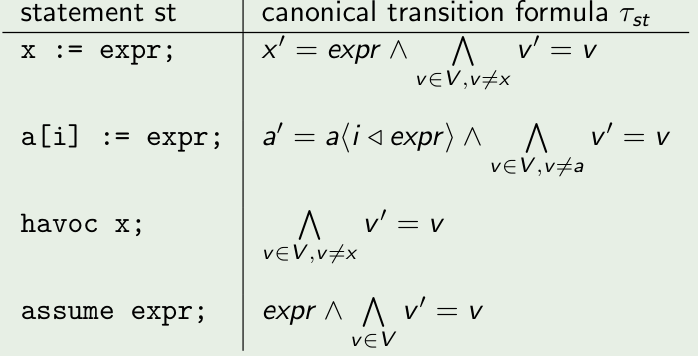
\includegraphics[width=0.5\linewidth]{./figures/transition_formulas.png}
					\item \underline{if bound is above and increasing:} \texttt{f(x, y) = 100 - x - y} for \texttt{while(x + y < 100)}
				\end{betterlist}
			}}
    \item Advantages and disadvantages.
		\framebox[0.90\textwidth][l]{\parbox{0.85\textwidth}{
        \begin{betterlist}
          \item[\color{green}{$\oplus$}] fully automatic
          \item[\color{green}{$\oplus$}] only really simple smt-solver calls, no qunators, not predicates, only first order logic variables (<=)
          \item[\color{green}{$\oplus$}] if there is a linear ranking function for a loop, then one will find it and thus if in a program all loops can be described by linear ranking functions one will prove termination for the program (relative completeness)
          \item[\color{green}{$\oplus$}] one gets a ranking function per loop and proofs termination if all loops have one, one has partial results if termination can not be proven
          \item[\color{red}{$\ominus$}] big restriction to linear ranking functions and for statements it has to be possible to bring them into a certain form of linear inequalities in matrix needed for Farkas lemma (no complete, many correct programs not provable, only for program with loops that can be described by one ultimately periodic trace)
          \item[\color{red}{$\ominus$}] cannot proof non-termination, because one only checks every loop for linera ranking function, but loop could have a non-linear ranking function
        \end{betterlist}
			}}
		\item Which kinds of specifications can be checked with the technique? E.g. precondition-postcondition pairs, assert statements, no division by zero, termination, ...

		\framebox[0.90\textwidth][l]{\parbox{0.85\textwidth}{
				\begin{betterlist}
					\item checking Termination (is undecidable)
				\end{betterlist}
			}}
		\item \alert{Soundness}
		\begin{betterlist}
			\item \underline{For correct programs}
			\begin{betterlist}
				\item In which circumstances does the technique claim that a program is correct?

				\framebox[0.90\textwidth][l]{\parbox{0.85\textwidth}{
						\begin{betterlist}
							\item If smt-solver able to satisfy constraints for all loops that they have a ranking function then the program is terminating (RankTerminate)
							\begin{betterlist}
								\item \alert{RankTerminate:} Let $P$ be a program. If every while loop of $P$ has a ranking function then $P$ is terminating
							\end{betterlist}
						\end{betterlist}
					}}
				\item Existence of false negatives: If the technique claims a program is correct, is the program guaranteed to be correct?

				\framebox[0.90\textwidth][l]{\parbox{0.85\textwidth}{
						\begin{betterlist}
							\item no, RankTerminate is an implication, conclusion is the case if premise satisfied
						\end{betterlist}
					}}
			\end{betterlist}
			\item \underline{For incorrect programs}
			\begin{betterlist}
				\item In which circumstances does the technique claim that a program is incorrect?

				\framebox[0.90\textwidth][l]{\parbox{0.85\textwidth}{
						\begin{betterlist}
							\item never, it always terminates with unknown for reason described below in the unknown section
						\end{betterlist}
					}}
				\item Existence of false positives: If the technique claims a program is incorrect, is the program guaranteed to be incorrect?

				\framebox[0.90\textwidth][l]{\parbox{0.85\textwidth}{
						\begin{betterlist}
							\item there are not true positives, thus also no false positives
						\end{betterlist}
					}}
			\end{betterlist}
			\item Which assumptions (on the program, or the specification, or the program’s environment) are needed for soundness?
			\framebox[0.90\textwidth][l]{\parbox{0.85\textwidth}{
					\begin{betterlist}
						\item Only works for ultimately periodic traces (= lasso traces), everyting else same as for invariant synthesis
						\begin{betterlist}
							\item only programs that have a statements that have a transition formula and can be brought in the right form for Farka's lemma (\texttt{while(x > 3)\{ x = x - 1\}})
						\end{betterlist}
					\end{betterlist}
				}}
		\end{betterlist}
		\item \alert{Completeness}
		\begin{betterlist}
			\item \underline{UNKNOWN verdicts} (failing to either establish correctness of incorrectness)
			\begin{betterlist}
				\item Given a correct program, is it possible that the technique terminates with an UNKNOWN verdict? If so, in which cases can this happen?

				\framebox[0.90\textwidth][l]{\parbox{0.85\textwidth}{
						\begin{betterlist}
							\item yes, becauee ranking function synthesis only find linear ranking function and it could be that the termination of the program can only be proven with a non-linear ranking function
						\end{betterlist}
					}}
				\item Given an incorrect program, is it possible that the technique terminates with an UNKNOWN verdict? If so, in which cases can this happen?

				\framebox[0.90\textwidth][l]{\parbox{0.85\textwidth}{
						\begin{betterlist}
							\item yes, incorrect programs always terminate with unknown, because ranking function synthesis can only find linear ranking functions and the program could still be correct and just have a non-linear ranking function
						\end{betterlist}
					}}
			\end{betterlist}
			\item \underline{Termination}
			\begin{betterlist}
				\item Does the technique always terminate for correct programs? If not, what might the technique do for an infinite amount of time (which step of the algorithm)? In which cases can this occur?

				\framebox[0.90\textwidth][l]{\parbox{0.85\textwidth}{
						\begin{betterlist}
							\item dependend Smt-solver, how long smt script with contraints needs to run through, but probably yes
						\end{betterlist}
					}}
				\item Does the technique always terminate for incorrect programs? If not, what might the technique do for an infinite amount of time (which step of the algorithm)? In which cases can this occur?

				\framebox[0.90\textwidth][l]{\parbox{0.85\textwidth}{
						\begin{betterlist}
							\item dependend Smt-solver, how long smt script with contraints needs to run through, but probably yes
						\end{betterlist}
					}}
			\end{betterlist}
			\item Are there any programs which the technique does not support at all?

			\framebox[0.90\textwidth][l]{\parbox{0.85\textwidth}{
					\begin{betterlist}
						\item same as under assumptions for soundness
					\end{betterlist}

				}}
		\end{betterlist}
		\item \alert{User Input:} How much / which user input is needed for the technique?
		\begin{betterlist}
			\item \checkboxChecked the program, converted to

			\framebox[0.90\textwidth][l]{\parbox{0.85\textwidth}{
					\begin{betterlist}
						\item Program automaton
					\end{betterlist}
				}}
			\item \checkboxHalfChecked the specification. Explain: Is the specification high-level or detailed, easy to specify or complex?

			\framebox[0.90\textwidth][l]{\parbox{0.85\textwidth}{
					\begin{betterlist}
						\item precondition-postcondition pair correctly specified for 2nd constraints
					\end{betterlist}
				}}
			\item \checkboxUnchecked suitable settings; e.g. choosing a mode or abstract domain for the given program and specification. Explain: What has to be chosen, and how easy is it to predict useful settings for a given program?

			\framebox[0.90\textwidth][l]{\parbox{0.85\textwidth}{
					-
				}}
			\item \checkboxUnchecked parts of the proof, e.g. invariants. Explain: What has to be given? Does it sometimes suffice to give parts, and the rest can be inferred?

			\framebox[0.90\textwidth][l]{\parbox{0.85\textwidth}{
					-
				}}
			\item \checkboxUnchecked individual steps of the proof, using some proof system. Explain: Which steps can be applied systematically? Where is creativity needed?

			\framebox[0.90\textwidth][l]{\parbox{0.85\textwidth}{
					-
				}}
			\item \checkboxUnchecked the proof is completely manual
			\framebox[0.90\textwidth][l]{\parbox{0.85\textwidth}{
					-
				}}
		\end{betterlist}
		\item \alert{Provided Output}
		\begin{betterlist}
			\item If the technique determines that a program is incorrect, what additional information can be provided to the user? E.g. a failing execution (including variable values), a feasible error trace, any information about why the program is incorrect?
			\framebox[0.90\textwidth][l]{\parbox{0.85\textwidth}{
					\begin{betterlist}
						\item it never determines that, only unknown
						\begin{betterlist}
							\item can return loop / trace for which linear ranking function couldn't be found
						\end{betterlist}

					\end{betterlist}

				}}
			\item If the technique determines that a program is correct, what additional information can be provided to the user? E.g. is there some kind of \enquote{proof artifact} that can be created? If so, is it easy to understand for humans? Is it usable by machines?

			\framebox[0.90\textwidth][l]{\parbox{0.85\textwidth}{
					\begin{betterlist}
						\item can get parameters through satisfying model for linear constraints in floyd hoare annotation
					\end{betterlist}
				}}
			\item If the technique returns UNKNOWN, what additional information can be provided to the user? Does the information help the user to understand why the result is UNKNOWN? Does it help the user to provide better input that avoids an UNKNOWN verdict?

			\framebox[0.90\textwidth][l]{\parbox{0.85\textwidth}{
					\begin{betterlist}
						\item can return loop / trace for which linear ranking function couldn't be found
					\end{betterlist}
				}}
			\item If the technique does not terminate or runs for a very long time, what information can be provided to help the user understand why?

			\framebox[0.90\textwidth][l]{\parbox{0.85\textwidth}{
					\begin{betterlist}
						\item dependant on smt-solver but most probably terminates, can return loop / trace for which linear ranking function couldn't be found
					\end{betterlist}
				}}
		\end{betterlist}
		\item \alert{Efficiency}
		\begin{betterlist}
			\item What are the bottlenecks for the technique? Which steps of the algorithm may be particularly inefficient, and in which cases?

			\framebox[0.90\textwidth][l]{\parbox{0.85\textwidth}{
					\begin{betterlist}
						\item (smt-solver calls for ranking function synthesis)
					\end{betterlist}
				}}
			\item Are there particularly important optimizations?

			\framebox[0.90\textwidth][l]{\parbox{0.85\textwidth}{
					-
				}}
		\end{betterlist}
		\item \alert{Further Aspects}
		\begin{betterlist}
			\item \underline{Modularity:} Can the verification for complex programs (or complex specifications) be broken down into verification tasks for smaller parts of the program / parts of the specification? If so, does this allow for efficiency benefits, e.g. parallelization of the sub-verification tasks? Can the modularity help as part of a software development process? E.g. by allowing to verify parts of the program, when other parts have not been written yet?

			\framebox[0.90\textwidth][l]{\parbox{0.85\textwidth}{
					-
				}}
			\item \underline{Incrementality:} Can verification artefacts be reused for modified versions of the program? E.g. if the program is still under development.

			\framebox[0.90\textwidth][l]{\parbox{0.85\textwidth}{
					-
				}}
			\item Which techniques are used? E.g. SMT solving, automata, ...

			\framebox[0.90\textwidth][l]{\parbox{0.85\textwidth}{
					\begin{betterlist}
						\item program automaton, Smt-solver for checking smt-script with constraints for ranking function synthesis
					\end{betterlist}
				}}
			\item How much is the overall cost of applying the technique? The cost may depend on how much computing power is needed, but often the cost for human labor (salary for skilled engineers who provide invariants or perform proofs) is much higher
			\framebox[0.90\textwidth][l]{\parbox{0.85\textwidth}{
					\begin{betterlist}
						\item dependant on smt-solver
					\end{betterlist}
				}}
		\end{betterlist}
	\end{betterlist}
\end{minipage}
%           \adjustbox{scale=0.5}{
%             % \begin{noindent}
%       \begin{dnumberedcodebox}[minted language=go,minted options={autogobble, fontsize=\tiny,numbersep=0.3cm,linenos}, box align=top]
% oldf1 := f1(x,y);
% oldf2 := f2(x,y);
% while (x>0 && y>0) {
%   if (*) {
%     x := x-1;
%     havoc y;
%   } else {
%     y := y-1;
%   }
%   assert (oldf1 > f1(x,y) && oldf1 >= 0)
%       || (oldf2 > f2(x,y) && oldf2 >= 0);
%   if (*) {
%     oldf1 := f1(x,y);
%     oldf2 := f2(x,y);
%   }
% }
%       \end{dnumberedcodebox}
%     %\end{noindent}
%           }
\begin{minipage}[t]{0.16\linewidth}
	\begin{myverbbox}{codeone}
		while (x>0 && y>0) {
				if (*) {
						x := x-1;
						havoc y;
					} else {
						y := y-1;
					}
				assert false;
			}
	\end{myverbbox}
	\begin{myverbbox}{codetwo}
		oldf1 := f1(x,y);
		oldf2 := f2(x,y);
		while (x>0 && y>0) {
				if (*) {
						x := x-1;
						havoc y;
					} else {
						y := y-1;
					}
				assert (oldf1 > f1(x,y) && oldf1 >= 0)
				|| (oldf2 > f2(x,y) && oldf2 >= 0);
				if (*) {
						oldf1 := f1(x,y);
						oldf2 := f2(x,y);
					}
			}
	\end{myverbbox}
	\begin{myverbbox}{codefour}
		oldx := fx(x);
		oldy := fy(x);
		while(x > 10){
				if(){
						x := x - 1;
						y := y + 2;
					} else {
						y := y - 1
						x := x + 2;
					}
				assert((fx(x) > oldx && oldx >= 0) || (fy(y) > oldy && oldy >= 0))
				if(*) {
						oldx := fx(x);
						oldy := fy(x);
					}
			}
	\end{myverbbox}
	\raggedright
	\fbox{Terminator}
	\begin{betterlist}
		% \item see page \pageref{pdf:terminator}
		\item Give a short description of the technique
		\framebox[0.90\textwidth][l]{\parbox{0.85\textwidth}{
				\begin{betterlist}
					\item \underline{Algorithm for checking termination. Idea of the approach of the Terminator tool:} Iteratively collect ranking functions until termination of all loops is shown
					\begin{enumerate}
						\item Start with the empty set of ranking functions
						\item Pick an ultimately periodic trace for which termination is not yet shown (if termination is not yet proven)
						\item Compute a ranking function for this trace and add it to our collection (if the trace does not have in infinite execution)
						\item Check if the collection of ranking functions is sufficient to prove termination and continue with the second step
					\end{enumerate}
					\item \underline{transform into a safety problem:}

					\codeone
					\codetwo
					\item it does not need one (possibly complicated) ranking function for each loop but that it can use a combination of several ranking functions to prove termination of a single loop, because of the theoretical basis of disjunctively well-founded transition invariants
					\begin{betterlist}
						\item the proof uses a combinatorial result called Ramsey’s theorem to show that in every infinite execution, at least one of the two ranking functions would have to decrease infinitely often
					\end{betterlist}
					\item For concluding termination the nondeterministic assignments to \texttt{oldf1} and \texttt{oldf1} are vital. The safety proof does not only show that in each iteration the function \texttt{f1} or the function \texttt{f2} is decreasing, the safety proof shows that between every two (not necessarily consecutive) visits of the loop head the function \texttt{f1} or the function \texttt{f2} is decreasing
					\begin{betterlist}
						\item issue is that when a function does not decrease, it may increase by an arbitrary amount, force the function to decrease / increase in the oppositive direction for the other variable, while the function is still decreasing for one variable in every step
					\end{betterlist}

					\codefour
				\end{betterlist}
			}}
    \item Advantages and disadvantages.
		\framebox[0.90\textwidth][l]{\parbox{0.85\textwidth}{
        \begin{betterlist}
          \item[\color{green}{$\oplus$}] fully automatic
          \item[\color{green}{$\oplus$}] can prove more complex loops that have multiple ultimately periodic traces, compared to simple ranking function synthesis
          \item[\color{green}{$\oplus$}] if there is loop with multiple ultimately periodic traces, then one will find all linear ranking functions and if all loop in a program have this property, then one will prove termination for this program (relative completeness)
          \item[\color{green}{$\oplus$}] one gets multiple linear ranking functions per loop that cover a possible more complicated ranking function and proofs termination if alll loops are covered, one has partial results if termination can not be proven
          \item[\color{red}{$\ominus$}] still big restriction to disjuntion of linear ranking functions and for statements it has to be possible to bring them into a certain form of linear inequalities in matrix needed for Farkas lemma (no complete, many correct programs not provable, only for programs with loops that can be described by ultimately periodic traces)
          \item[\color{red}{$\ominus$}] cannot proof non-termination, because one only checks every loop for linera ranking functions, but loop could have a non-linear ranking function not desribable by disjunction of multiple linear ranking functions
        \end{betterlist}
			}}
		\item Which kinds of specifications can be checked with the technique? E.g. precondition-postcondition pairs, assert statements, no division by zero, termination, ...

		\framebox[0.90\textwidth][l]{\parbox{0.85\textwidth}{
				\begin{betterlist}
					\item checking Termination (is undecidable)
				\end{betterlist}
			}}
		\item \alert{Soundness}
		\begin{betterlist}
			\item \underline{For correct programs}
			\begin{betterlist}
				\item In which circumstances does the technique claim that a program is correct?

				\framebox[0.90\textwidth][l]{\parbox{0.85\textwidth}{
						\begin{betterlist}
							\item If one is able to find a ranking function for every ultimately periodic trace, then the program is terminating, because of the theoretical basis of disjunctively well-founded transition invariants
						\end{betterlist}
					}}
				\item Existence of false negatives: If the technique claims a program is correct, is the program guaranteed to be correct?

				\framebox[0.90\textwidth][l]{\parbox{0.85\textwidth}{
						\begin{betterlist}
							\item yes, because RankTerminate is an implication
							\begin{betterlist}
								\item \alert{RankTerminate:} Let $P$ be a program. If every while loop of $P$ has a ranking function then $P$ is terminating
							\end{betterlist}
						\end{betterlist}
					}}
			\end{betterlist}
			\item \underline{For incorrect programs}
			\begin{betterlist}
				\item In which circumstances does the technique claim that a program is incorrect?

				\framebox[0.90\textwidth][l]{\parbox{0.85\textwidth}{
						\begin{betterlist}
							\item never, if it doesn't find ranking function, unknown, becase one is only checking if there's linear ranking function, but there could be non-linear ranking function
							% \item Can't detect every terminating program
							% \begin{betterlist}
							% \item can't check non-termination
							% \end{betterlist}
						\end{betterlist}
					}}
				\item Existence of false positives: If the technique claims a program is incorrect, is the program guaranteed to be incorrect?

				\framebox[0.90\textwidth][l]{\parbox{0.85\textwidth}{
						\begin{betterlist}
							\item there are not true positives, thus there are also no false positives
						\end{betterlist}
					}}
			\end{betterlist}
			\item Which assumptions (on the program, or the specification, or the program’s environment) are needed for soundness?
			\framebox[0.90\textwidth][l]{\parbox{0.85\textwidth}{
					\begin{betterlist}
						\item loops only contain ultimately periodic traces that can be descibed by linear ranking functions
						\item every statement in the loops needs to have a transition formula and if the 2nd constraint for ranking functions is used, then also all statements before the loop (stam)
						\item it has to be possible to write every statement in matrix notation needed for Farka's lemma (\texttt{x := x * y} can't be written as two inequalities of the form $r_x \cdot x + r_y\cdot y \le r_0$)
					\end{betterlist}
				}}
		\end{betterlist}
		\item \alert{Completeness}
		\begin{betterlist}
			\item \underline{UNKNOWN verdicts} (failing to either establish correctness of incorrectness)
			\begin{betterlist}
				\item Given a correct program, is it possible that the technique terminates with an UNKNOWN verdict? If so, in which cases can this happen?

				\framebox[0.90\textwidth][l]{\parbox{0.85\textwidth}{
						\begin{betterlist}
							\item yes, if a loops of a correct program can't be described by linear ranking functions, there could be a non-linear ranking function, so one can't say whether it's terminating or non-terminating
							\item (also a bad smt-solver can return unknown)
						\end{betterlist}
					}}
				\item Given an incorrect program, is it possible that the technique terminates with an UNKNOWN verdict? If so, in which cases can this happen?

				\framebox[0.90\textwidth][l]{\parbox{0.85\textwidth}{
						\begin{betterlist}
							\item for incorrect programs it always terminates with unknown for the same reason as above
						\end{betterlist}
					}}
			\end{betterlist}
			\item \underline{Termination}
			\begin{betterlist}
				\item Does the technique always terminate for correct programs? If not, what might the technique do for an infinite amount of time (which step of the algorithm)? In which cases can this occur?

				\framebox[0.90\textwidth][l]{\parbox{0.85\textwidth}{
						\begin{betterlist}
							% \item yes, there are ony finitely many loops with linear ranking function
							\item no, it's possible that it's always able to find a linear ranking function, but it could find infintely many ultimately periodic traces / lassos and Terminator may never find a finite collection of linear ranking functions that are suitable to show termination for all lassos
							\item but may use timeouts
						\end{betterlist}
					}}
				\item Does the technique always terminate for incorrect programs? If not, what might the technique do for an infinite amount of time (which step of the algorithm)? In which cases can this occur?

				\framebox[0.90\textwidth][l]{\parbox{0.85\textwidth}{
						\begin{betterlist}
							% \item yes, if there's no linear ranking function found by invariant synthesis, smt-solver says unsatasfiable, no linear ranking function can be found, then the program terminates
							\item no, same as above
							\item but may use timeouts
						\end{betterlist}
					}}
			\end{betterlist}
			\item Are there any programs which the technique does not support at all?

			\framebox[0.90\textwidth][l]{\parbox{0.85\textwidth}{
					\begin{betterlist}
						\item Only program whose statements can be brought in a form such that Farka's lemma can be applied (this matrix notation) and only loops for which there are linear ranking functions describing their ultimately periodic traces (because of ranking function synthesis using Farka's lemma)
						\begin{betterlist}
							\item can check while loops with if else
						\end{betterlist}
					\end{betterlist}
				}}
		\end{betterlist}
		\item \alert{User Input:} How much / which user input is needed for the technique?
		\begin{betterlist}
			\item \checkboxChecked the program, converted to

			\framebox[0.90\textwidth][l]{\parbox{0.85\textwidth}{
					\begin{betterlist}
						\item Program automaton
					\end{betterlist}
				}}
			\item \checkboxHalfChecked the specification. Explain: Is the specification high-level or detailed, easy to specify or complex?

			\framebox[0.90\textwidth][l]{\parbox{0.85\textwidth}{
					\begin{betterlist}
						\item precondition-postcondition pair correctly specified for 2nd constraints
					\end{betterlist}
				}}
			\item \checkboxUnchecked suitable settings; e.g. choosing a mode or abstract domain for the given program and specification. Explain: What has to be chosen, and how easy is it to predict useful settings for a given program?

			\framebox[0.90\textwidth][l]{\parbox{0.85\textwidth}{
					-
				}}
			\item \checkboxUnchecked parts of the proof, e.g. invariants. Explain: What has to be given? Does it sometimes suffice to give parts, and the rest can be inferred?

			\framebox[0.90\textwidth][l]{\parbox{0.85\textwidth}{
					-
				}}
			\item \checkboxUnchecked individual steps of the proof, using some proof system. Explain: Which steps can be applied systematically? Where is creativity needed?

			\framebox[0.90\textwidth][l]{\parbox{0.85\textwidth}{
					-
				}}
			\item \checkboxUnchecked the proof is completely manual
			\framebox[0.90\textwidth][l]{\parbox{0.85\textwidth}{
					-
				}}
		\end{betterlist}
		\item \alert{Provided Output}
		\begin{betterlist}
			\item If the technique determines that a program is incorrect, what additional information can be provided to the user? E.g. a failing execution (including variable values), a feasible error trace, any information about why the program is incorrect?

			\framebox[0.90\textwidth][l]{\parbox{0.85\textwidth}{
					\begin{betterlist}
						\item it never determines that, for incorrect non-terminating programs it always returns unknown
						\begin{betterlist}
							\item for unknown ranking functions found so far and trace for which it couldn't be found
						\end{betterlist}
					\end{betterlist}
				}}
			\item If the technique determines that a program is correct, what additional information can be provided to the user? E.g. is there some kind of \enquote{proof artifact} that can be created? If so, is it easy to understand for humans? Is it usable by machines?

			\framebox[0.90\textwidth][l]{\parbox{0.85\textwidth}{
					\begin{betterlist}
						\item Get ranking function for all whiles and thus proofs for termination (by RankTerminate)
					\end{betterlist}
				}}
			\item If the technique returns UNKNOWN, what additional information can be provided to the user? Does the information help the user to understand why the result is UNKNOWN? Does it help the user to provide better input that avoids an UNKNOWN verdict?

			\framebox[0.90\textwidth][l]{\parbox{0.85\textwidth}{
					\begin{betterlist}
						\item get ranking functions found so far and returns ultimately periodic trace for which it couldn't find linear ranking function, so user can try to find one manually
					\end{betterlist}
				}}
			\item If the technique does not terminate or runs for a very long time, what information can be provided to help the user understand why?

			\framebox[0.90\textwidth][l]{\parbox{0.85\textwidth}{
					\begin{betterlist}
						\item is always terminating, if it doesn't find a linear ranking function it stops
					\end{betterlist}
				}}
		\end{betterlist}
		\item \alert{Efficiency}
		\begin{betterlist}
			\item What are the bottlenecks for the technique? Which steps of the algorithm may be particularly inefficient, and in which cases?

			\framebox[0.90\textwidth][l]{\parbox{0.85\textwidth}{
					\begin{betterlist}
						\item (Smt-solver for ranking function synthesis)
					\end{betterlist}
				}}
			\item Are there particularly important optimizations?

			\framebox[0.90\textwidth][l]{\parbox{0.85\textwidth}{
					\begin{betterlist}
						\item T2 tool
					\end{betterlist}
				}}
		\end{betterlist}
		\item \alert{Further Aspects}
		\begin{betterlist}
			\item \underline{Modularity:} Can the verification for complex programs (or complex specifications) be broken down into verification tasks for smaller parts of the program / parts of the specification? If so, does this allow for efficiency benefits, e.g. parallelization of the sub-verification tasks? Can the modularity help as part of a software development process? E.g. by allowing to verify parts of the program, when other parts have not been written yet?

			\framebox[0.90\textwidth][l]{\parbox{0.85\textwidth}{
					\begin{betterlist}
						\item yes, loop invariants of two different loops can be analysed in whatever order% if first constraints are enough, for 2nd constraints only if new loop invariant is a stronger of the 2nd loop invariant
						\prepostreusetwo for 2nd constraint
					\end{betterlist}
				}}
			\item \underline{Incrementality:} Can verification artefacts be reused for modified versions of the program? E.g. if the program is still under development.

			\framebox[0.90\textwidth][l]{\parbox{0.85\textwidth}{
					\begin{betterlist}
						\item reuse ranking functions already found if one used first constraints for ranking function synthesis (is going to work with every invariant), don't have to find one again, but if used seconds constraints one needs to have the same invariant to be the case before the while loop
					\end{betterlist}
				}}
			\item Which techniques are used? E.g. SMT solving, automata, ...

			\framebox[0.90\textwidth][l]{\parbox{0.85\textwidth}{
					\begin{betterlist}
						\item constructing program automatons, smt-solver calls
					\end{betterlist}
				}}
			\item How much is the overall cost of applying the technique? The cost may depend on how much computing power is needed, but often the cost for human labor (salary for skilled engineers who provide invariants or perform proofs) is much higher
			\framebox[0.90\textwidth][l]{\parbox{0.85\textwidth}{
					\begin{betterlist}
						\item dependant on smt-solver
					\end{betterlist}
				}}
		\end{betterlist}
	\end{betterlist}
\end{minipage}
\begin{minipage}[t]{0.16\linewidth}
	\raggedright
	\fbox{Template}
	\begin{betterlist}
		\item Give a short description of the technique
		\framebox[0.90\textwidth][l]{\parbox{0.85\textwidth}{
				\begin{betterlist}
					\item TODO
				\end{betterlist}
			}}
    \item Advantages and disadvantages.
		\framebox[0.90\textwidth][l]{\parbox{0.85\textwidth}{
        \begin{betterlist}
          \item[\color{green}{$\oplus$}] 
          \item[\color{red}{$\ominus$}] 
        \end{betterlist}
			}}
		\item Which kinds of specifications can be checked with the technique? E.g. precondition-postcondition pairs, assert statements, no division by zero, termination, ...

		\framebox[0.90\textwidth][l]{\parbox{0.85\textwidth}{
				\begin{betterlist}
					\item TODO
				\end{betterlist}
			}}
		\item \alert{Soundness}
		\begin{betterlist}
			\item \underline{For correct programs}
			\begin{betterlist}
				\item In which circumstances does the technique claim that a program is correct?

				\framebox[0.90\textwidth][l]{\parbox{0.85\textwidth}{
						\begin{betterlist}
							\item TODO
						\end{betterlist}
					}}
				\item Existence of false negatives: If the technique claims a program is correct, is the program guaranteed to be correct?

				\framebox[0.90\textwidth][l]{\parbox{0.85\textwidth}{
						\begin{betterlist}
							\item TODO
						\end{betterlist}
					}}
			\end{betterlist}
			\item \underline{For incorrect programs}
			\begin{betterlist}
				\item In which circumstances does the technique claim that a program is incorrect?

				\framebox[0.90\textwidth][l]{\parbox{0.85\textwidth}{
						\begin{betterlist}
							\item TODO
						\end{betterlist}
					}}
				\item Existence of false positives: If the technique claims a program is incorrect, is the program guaranteed to be incorrect?

				\framebox[0.90\textwidth][l]{\parbox{0.85\textwidth}{
						\begin{betterlist}
							\item TODO
						\end{betterlist}
					}}
			\end{betterlist}
			\item Which assumptions (on the program, or the specification, or the program’s environment) are needed for soundness?
			\framebox[0.90\textwidth][l]{\parbox{0.85\textwidth}{
					\begin{betterlist}
						\item TODO
					\end{betterlist}
				}}
		\end{betterlist}
		\item \alert{Completeness}
		\begin{betterlist}
			\item \underline{UNKNOWN verdicts} (failing to either establish correctness of incorrectness)
			\begin{betterlist}
				\item Given a correct program, is it possible that the technique terminates with an UNKNOWN verdict? If so, in which cases can this happen?

				\framebox[0.90\textwidth][l]{\parbox{0.85\textwidth}{
						\begin{betterlist}
							\item TODO
						\end{betterlist}
					}}
				\item Given an incorrect program, is it possible that the technique terminates with an UNKNOWN verdict? If so, in which cases can this happen?

				\framebox[0.90\textwidth][l]{\parbox{0.85\textwidth}{
						\begin{betterlist}
							\item TODO
						\end{betterlist}
					}}
			\end{betterlist}
			\item \underline{Termination}
			\begin{betterlist}
				\item Does the technique always terminate for correct programs? If not, what might the technique do for an infinite amount of time (which step of the algorithm)? In which cases can this occur?

				\framebox[0.90\textwidth][l]{\parbox{0.85\textwidth}{
						\begin{betterlist}
							\item TODO
						\end{betterlist}
					}}
				\item Does the technique always terminate for incorrect programs? If not, what might the technique do for an infinite amount of time (which step of the algorithm)? In which cases can this occur?

				\framebox[0.90\textwidth][l]{\parbox{0.85\textwidth}{
						\begin{betterlist}
							\item TODO
						\end{betterlist}
					}}
			\end{betterlist}
			\item Are there any programs which the technique does not support at all?

			\framebox[0.90\textwidth][l]{\parbox{0.85\textwidth}{
					\begin{betterlist}
						\item TODO
					\end{betterlist}
				}}
		\end{betterlist}
		\item \alert{User Input:} How much / which user input is needed for the technique?
		\begin{betterlist}
			\item \checkboxChecked the program, converted to

			\framebox[0.90\textwidth][l]{\parbox{0.85\textwidth}{
					\begin{betterlist}
						\item CFG
					\end{betterlist}
				}}
			\item \checkboxHalfChecked the specification. Explain: Is the specification high-level or detailed, easy to specify or complex?

			\framebox[0.90\textwidth][l]{\parbox{0.85\textwidth}{
					\begin{betterlist}
						\item TODO
					\end{betterlist}
				}}
			\item \checkboxUnchecked suitable settings; e.g. choosing a mode or abstract domain for the given program and specification. Explain: What has to be chosen, and how easy is it to predict useful settings for a given program?

			\framebox[0.90\textwidth][l]{\parbox{0.85\textwidth}{
					\begin{betterlist}
						\item TODO
					\end{betterlist}
				}}
			\item \checkboxUnchecked parts of the proof, e.g. invariants. Explain: What has to be given? Does it sometimes suffice to give parts, and the rest can be inferred?

			\framebox[0.90\textwidth][l]{\parbox{0.85\textwidth}{
					\begin{betterlist}
						\item TODO
					\end{betterlist}
				}}
			\item \checkboxUnchecked individual steps of the proof, using some proof system. Explain: Which steps can be applied systematically? Where is creativity needed?

			\framebox[0.90\textwidth][l]{\parbox{0.85\textwidth}{
					\begin{betterlist}
						\item TODO
					\end{betterlist}
				}}
			\item \checkboxUnchecked the proof is completely manual
			\framebox[0.90\textwidth][l]{\parbox{0.85\textwidth}{
					\begin{betterlist}
						\item TODO
					\end{betterlist}
				}}
		\end{betterlist}
		\item \alert{Provided Output}
		\begin{betterlist}
			\item If the technique determines that a program is incorrect, what additional information can be provided to the user? E.g. a failing execution (including variable values), a feasible error trace, any information about why the program is incorrect?

			\framebox[0.90\textwidth][l]{\parbox{0.85\textwidth}{
					\begin{betterlist}
						\item TODO
					\end{betterlist}
				}}
			\item If the technique determines that a program is correct, what additional information can be provided to the user? E.g. is there some kind of \enquote{proof artifact} that can be created? If so, is it easy to understand for humans? Is it usable by machines?

			\framebox[0.90\textwidth][l]{\parbox{0.85\textwidth}{
					\begin{betterlist}
						\item TODO
					\end{betterlist}
				}}
			\item If the technique returns UNKNOWN, what additional information can be provided to the user? Does the information help the user to understand why the result is UNKNOWN? Does it help the user to provide better input that avoids an UNKNOWN verdict?

			\framebox[0.90\textwidth][l]{\parbox{0.85\textwidth}{
					\begin{betterlist}
						\item TODO
					\end{betterlist}
				}}
			\item If the technique does not terminate or runs for a very long time, what information can be provided to help the user understand why?

			\framebox[0.90\textwidth][l]{\parbox{0.85\textwidth}{
					\begin{betterlist}
						\item TODO
					\end{betterlist}
				}}
		\end{betterlist}
		\item \alert{Efficiency}
		\begin{betterlist}
			\item What are the bottlenecks for the technique? Which steps of the algorithm may be particularly inefficient, and in which cases?

			\framebox[0.90\textwidth][l]{\parbox{0.85\textwidth}{
					\begin{betterlist}
						\item TODO
					\end{betterlist}
				}}
			\item Are there particularly important optimizations?

			\framebox[0.90\textwidth][l]{\parbox{0.85\textwidth}{
					\begin{betterlist}
						\item TODO
					\end{betterlist}
				}}
		\end{betterlist}
		\item \alert{Further Aspects}
		\begin{betterlist}
			\item \underline{Modularity:} Can the verification for complex programs (or complex specifications) be broken down into verification tasks for smaller parts of the program / parts of the specification? If so, does this allow for efficiency benefits, e.g. parallelization of the sub-verification tasks? Can the modularity help as part of a software development process? E.g. by allowing to verify parts of the program, when other parts have not been written yet?

			\framebox[0.90\textwidth][l]{\parbox{0.85\textwidth}{
					\begin{betterlist}
						\item TODO
					\end{betterlist}
				}}
			\item \underline{Incrementality:} Can verification artefacts be reused for modified versions of the program? E.g. if the program is still under development.

			\framebox[0.90\textwidth][l]{\parbox{0.85\textwidth}{
					\begin{betterlist}
						\item TODO
					\end{betterlist}
				}}
			\item Which techniques are used? E.g. SMT solving, automata, ...

			\framebox[0.90\textwidth][l]{\parbox{0.85\textwidth}{
					\begin{betterlist}
						\item TODO
					\end{betterlist}
				}}
			\item How much is the overall cost of applying the technique? The cost may depend on how much computing power is needed, but often the cost for human labor (salary for skilled engineers who provide invariants or perform proofs) is much higher
			\framebox[0.90\textwidth][l]{\parbox{0.85\textwidth}{
					\begin{betterlist}
						\item TODO
					\end{betterlist}
				}}
		\end{betterlist}
	\end{betterlist}
\end{minipage}

% \phantomsection
% \addcontentsline{toc}{section}{Relational Semantics}
% \includepdf[pages=-]{./content/Theo_questionnaire-relational_semantics.pdf}
% \label{pdf:relational_semantics}
%
%
% \newpage
% \phantomsection
% \addcontentsline{toc}{section}{Hoare Proof System}
% \includepdf[pages=-]{./content/Theo_questionnaire-hoare_proof_system.pdf}
% \label{pdf:hoare_proof_system}
%
% \newpage
% \phantomsection
% \addcontentsline{toc}{section}{Explicit State Model Checking}
% \includepdf[pages=-]{./content/Theo_questionnaire-explicit_state_model_checking.pdf}
% \label{pdf:explicit_state_model_checking}
%
% \newpage
% \phantomsection
% \addcontentsline{toc}{section}{Bounded Model Checking}
% \includepdf[pages=-]{./content/Theo_questionnaire-bounded_mode_checking.pdf}
% \label{pdf:bounded_mode_checking}
%
% \newpage
% \phantomsection
% \addcontentsline{toc}{section}{Invariant Synthesis}
% \includepdf[pages=-]{./content/Theo_questionnaire-invariant_synthesis.pdf}
% \label{pdf:invariant_synthesis}
%
% \newpage
% \phantomsection
% \addcontentsline{toc}{section}{Ranking Function Synthesis}
% \includepdf[pages=-]{./content/Theo_questionnaire-ranking_function_synthesis.pdf}
% \label{pdf:ranking_function_synthesis}
%
% \newpage
% \phantomsection
% \addcontentsline{toc}{section}{Terminator}
% \includepdf[pages=-]{./content/Terminator.pdf}
% \label{pdf:terminator}
%
% \newpage
% \phantomsection
% \addcontentsline{toc}{section}{Credits}
% \fbox{Credits}
% \begin{betterlist}
% 	\item \alert{Theo:} Hoare Proof System, Explicit-State Model Checking, Bounded Model Checking, Invariant Synthesis, Ranking Function Synthesis
% 	\item \alert{Jürgen:} Abstract Interpretion, CEGAR, Trace Abstraction
% 	\item \alert{Aisan:} Terminator
% \end{betterlist}
\end{document}
